\documentclass[a4paper,12p]{article}
\usepackage[utf8]{inputenc}
\usepackage[ngerman]{babel}
\usepackage[a4paper, left=2.5cm, right=2.5cm]{geometry}
\usepackage{amsmath}
\usepackage{tikz}
\usepackage{graphicx}
\usepackage{mathtools}
\usepackage{cancel}
\usepackage{amssymb}


\title{\huge Modellbildung\\\large \huge Beispielsammlung}
\author{\huge 4.Semester ET-Studium}
\date{\huge Oktober 2019}

\begin{document}

	\maketitle
	\newpage
	\tableofcontents
	\newpage
	
	\section{Einleitung}
	In dieser Ausarbeitung befinden sich sämtliche Rechenwege der Modellbildungsprüfung beginnend ab dem Jahr 2015. Die Angaben zu den hier ausgearbeiteten Prüfungen befinden sich auf der Homepage des ACIN. Sämtlichen verwendeten Formeln befinden sich in der Formelsammlung, welche ebenfalls auf der Homepage des ACIN zu finden ist. Zeichnungen wurden hier beifügt, sofern dies auch möglich war. Diese Sammlung soll dabei helfen schneller auf den Lösungsweg kommen. Es wird öfters vorkommen das die Lösung hier mit der Lösung aus der Musterlösung des Instituts nicht übereinstimmt. Manche Unterpunkte werden nicht gelöst, da zu diesen keine Musterlösungen. existeren. Die Berechnungen wurden großteils mit MAPLE berechnet und die nicht so aufwendigen Rechenschritte wurden detailiert in diese Ausarbeitung beschrieben.
	
	\section{Prüfungen}
	
	\subsection{26.06.2015}
	\textbf{Beispiel 1} \\ \\
a)\\ \\
Die generalisierten Koordinaten lauten
\[
	\textbf{q} = \left[ \begin{matrix}
		\varphi \\
		\psi
	\end{matrix}\right]
\]
Diese beiden sind deswegen die geeigneten generalisierten Koordinaten, weil diese sich mit der Zeit ändern können. \\ 
Die beiden Ortsvektoren $\textbf{r}_2$ und $\textbf{r}_K$ werden direkt aus Angabe abgelesen.
\[
	\textbf{r}_2 = \left[\begin{matrix}
		\frac{1}{2} L_2 + L_1 \sin\varphi \\
		-L_1\cos\varphi
	\end{matrix}\right] , 
	\textbf{r}_K = \left[\begin{matrix}
		\frac{1}{2} L_2 + L_1\sin\varphi + l\sin\psi \\
		-L_1\cos\varphi - l\cos\psi
	\end{matrix}\right]
\]
b) \\ \\
Den translatorische Geschwindigkeitsvektor erhält man durch die zeitliche Ableitung des entsprechenden Ortsvektors.
\[
	\dot{\textbf{r}}_K = \underbrace{L_1\dot{\varphi}\left[\begin{matrix}
		\cos\varphi \\
		\sin\varphi
	\end{matrix}\right]}_{\dot{\textbf{r}}_2}
	+
	l\dot{\psi}\left[\begin{matrix}
		\cos\psi\\
		\sin\psi
	\end{matrix}\right]
\]
c) \\ \\
Zwischenrechnungen für die Ermittlung der kinetischen Energie:
\begin{align*}
	\dot{\textbf{r}}_2^T\textbf{r}_2 &= L_1^2 \dot{\varphi}^2 \left[\begin{matrix}
	 \cos\varphi & \sin\varphi
	\end{matrix}\right]
	\left[\begin{matrix}
		\cos\varphi \\
		\sin\varphi
	\end{matrix}\right] \\
	&= L_1^2\dot{\varphi}^2\underbrace{\left(\cos^2\varphi + \sin^2\varphi\right)}_{=1} \\
	&= L_1^2\dot{\varphi}^2
\end{align*}
\begin{align*}
	\dot{\textbf{r}}_K^T\textbf{r}_K &= \left(L_1\dot{\varphi}\left[\begin{matrix}
		\cos\varphi &
		\sin\varphi
		\end{matrix}\right]
	+
	l\dot{\psi}\left[\begin{matrix}
	\cos\psi &
	\sin\psi
	\end{matrix}\right]\right)
	\left(L_1\dot{\varphi}\left[\begin{matrix}
		\cos\varphi \\
		\sin\varphi
		\end{matrix}\right]
	+
	l\dot{\psi}\left[\begin{matrix}
	\cos\psi\\
	\sin\psi
	\end{matrix}\right]\right) \\
	&= L_1^2\dot{\varphi}^2\underbrace{\left(\cos^2\varphi + \sin^2\varphi\right)}_{=1} + l^2\dot{\psi}^2\underbrace{\left( \cos^2\psi + \sin^2\psi\right)}_{=1} + 2L_1l\left(\sin\varphi\sin\psi + \cos\varphi\cos\psi\right) \\
	&= L_1^2\dot{\varphi}^2 + l^2\dot{\psi}^2 + 2L_1l\dot{\varphi}\dot{\psi}\left(\sin\varphi\sin\psi + \cos\varphi\cos\psi\right)
\end{align*}
\newpage
Nun können die kinetischen Energien des Systems bestimmt werden. Diese lauten hier
\begin{align*}
	T_{tr} &= \frac{1}{2} \left(m_2 + m_M\right) L_1^2\dot{\varphi}^2 + \frac{1}{2} m_K \left[ L_1^2\dot{\varphi}^2 + l^2\dot{\psi}^2 + 2L_1l\dot{\varphi}\dot{\psi}\left(\sin\varphi\sin\psi + \cos\varphi\cos\psi\right)\right] \\
	T_{rot} &= 2 \frac{1}{2} \left(\frac{1}{12}m_1L_1^2 + m_1\left(\frac{L_1}{2}\right)^2\right)\dot{\varphi}^2 \\
	T &= T_{tr} + T_{rot} \\
	  &= \frac{1}{2} \left(m_2 + m_M\right) L_1^2\dot{\varphi}^2 + \frac{1}{2} m_K \left[ L_1^2\dot{\varphi}^2 + l^2\dot{\psi}^2 + 2L_1l\dot{\varphi}\dot{\psi}\left(\sin\varphi\sin\psi + \cos\varphi\cos\psi\right)\right] \\
	  &+ 2\frac{1}{2} \left(\frac{1}{12}m_1L_1^2 + m_1\left(\frac{L_1}{2}\right)^2\right)\dot{\varphi}^2
\end{align*}
d) \\ \\
Nun kann wie folgt die potentielle Energie bestimmt werden. Die potentielle Energie der Ruhelage lautet
\begin{align*}
	V &= 2m_1g\frac{L_1}{2}\left(1-\cos\varphi\right) + \left(m_2 + m_M\right)gL_1 \left(1 - \cos\varphi\right) \\
	&+ m_Kg\left[L_1\left(1-\cos\varphi\right) +l\left(1 - \cos\psi\right)\right] + 2 \frac{1}{2}c_1\varphi^2
\end{align*}
\textit{Hinweis}: \\
Die Ruhelage befindet sich bei \(\varphi = 0\), d.h. das Maximum der potentiellen Energie tritt bei \(\varphi = \pm \frac{\pi}{2}\) und deswegen wird \(\cos\varphi\) durch \(\left(1-\cos\varphi\right)\) ersetzt. \\ \\
e) \\ \\
Um die Bewegungsgleichungen zu bestimmen, benötigt man als erstes aller erstes die Langrange-Funktion die wie folgt lautet
\begin{align*}
	L &= T - V \\
	  &= \frac{1}{2} \left(m_2 + m_M\right) L_1^2\dot{\varphi}^2 + \frac{1}{2} m_K \left[ L_1^2\dot{\varphi}^2 + l^2\dot{\psi}^2 + 2L_1l\dot{\varphi}\dot{\psi}\left(\sin\varphi\sin\psi + \cos\varphi\cos\psi\right)\right] 
	  + 2\frac{1}{2} \left(\frac{1}{12}m_1L_1^2 + m_1\left(\frac{L_1}{2}\right)^2\right)\dot{\varphi}^2 \\
	  &- 2m_1g\frac{L_1}{2}\left(1-\cos\varphi\right) - \left(m_2 + m_M\right)gL_1 \left(1 - \cos\varphi\right) - m_Kg\left[L_1\left(1-\cos\varphi\right) - l\left(1 - \cos\psi\right)\right] - 2 \frac{1}{2}c_1\varphi^2
\end{align*}
Als nächstes benötigt man die generalisierten Kräfte die hier wie folgt lauten
\[
	\textbf{f}_q = \left[\begin{matrix}
		-2d_1\varphi \\
		\tau
	\end{matrix}\right]
\]
Nun wertet man den Euler-Lagrange-Formalismus aus, der hier folgendermaßen aussieht
\begin{align*}
	\frac{d}{dt}\left(\frac{\partial L}{\partial \dot{\varphi}}\right) - \left(\frac{\partial L}{\partial \varphi}\right) &= -2d_1\dot{\varphi}\\
	\frac{d}{dt}\left(\frac{\partial L}{\partial \dot{\psi}}\right) - \left(\frac{\partial L}{\partial \psi }\right) &= \tau
\end{align*}
\newpage
\noindent
partiellen Ableitungen \\ \\
1. generalisierte Koordinate:
\begin{align*}
	\frac{\partial L}{\partial \dot{\varphi}} &= \left(m_2 + m_M\right)L_1^2\dot{\varphi} + m_K \left( L_1^2\dot{\varphi} + L_1l\dot{\psi}\left(\sin\varphi \sin\psi + \cos \varphi \cos\psi\right)\right) + 2\left(\frac{1}{12}m_1L_1^2 + m_1\left(\frac{L_1}{2}\right)^2\right)\dot{\varphi} \\
	\frac{d}{dt}\left(\frac{\partial L}{\partial \dot{\varphi}}\right) &= \left(m_2 + m_M\right)L_1^2 \ddot{\varphi} + m_K \left( L_1^2\ddot{\varphi} + L_1l\frac{d}{dt}\left(\dot{\psi}\left(\sin\varphi \sin\psi + \cos \varphi \cos\psi\right)\right)\right) + 2\left(\frac{1}{12}m_1L_1^2 + m_1\left(\frac{L_1}{2}\right)^2\right)\ddot{\varphi}\\
	&= \left( 2\left(\frac{1}{12}m_1L_1^2 + m_1\left(\frac{L_1}{2}\right)^2\right) + \left( m_2 + m_M + m_K\right)\right)\ddot{\varphi} + m_K L_1 \frac{d}{dt}\left(\psi\left(\sin\varphi \sin\psi + \cos\varphi \cos\psi\right)\right) \\
	\frac{\partial L}{\partial \varphi} &= m_KL_1l\dot{\varphi}\dot{\psi}\left(\cos\varphi \sin\psi + \sin\varphi \cos\psi\right)-m_1gL_1\sin\varphi - \left(m_2 + m_M\right)L_1g - m_KgL_1\sin\varphi - 2c_1\varphi \\
	&= m_KL_1l\dot{\varphi}\dot{\psi}\left(\cos\varphi \sin\psi + \sin\varphi \cos\psi\right) - \left(m_1 + m_M + m_2 + m_K\right)gL_1 - 2c_1\varphi
\end{align*}
2. generalisierte Koordinate:
\begin{align*}
	\frac{\partial L}{\partial \dot{\psi}} &= m_Kl^2\dot{\psi} + m_KL_1 \dot{\varphi}\left(\sin\varphi \sin\psi + \cos\varphi \cos\psi\right) \\
	\frac{d}{dt} \left(\frac{\partial L}{\partial \dot{\psi} }\right) &= m_Kl^2\ddot{\psi} + m_KL_1 \frac{d}{dt}\left(\dot{\varphi}\left(\sin\varphi \sin\psi + \cos\varphi \cos\psi\right)\right) \\
	\frac{\partial L}{\partial \psi} &= m_KL_1l\dot{\varphi}\dot{\psi}\left(\sin\varphi \cos\psi - \cos\varphi \sin\psi\right) - m_Kgl\sin\psi
\end{align*}
Somit lauten die Bewegungsgleichungen
\begin{align*}
	\left(2\left(\frac{1}{12}m_1L_1^2 + m_1\left(\frac{L_1}{2}\right)^2\right) + \left( m_2 + m_M + m_K\right)\right)\ddot{\varphi} + m_K L_1 \frac{d}{dt}\left(\psi\left(\sin\varphi \sin\psi + \cos\varphi \cos\psi\right)\right) \\
	- m_KL_1l\dot{\varphi}\dot{\psi}\left(\cos\varphi \sin\psi + \sin\varphi \cos\psi\right) + \left(m_1 + m_M + m_2 + m_K\right)gL_1 + 2c_1\varphi = -2d_1\dot{\varphi}
\end{align*}
\begin{align*}
	m_Kl^2\ddot{\psi} + m_KL_1 \frac{d}{dt}\left(\dot{\varphi}\left(\sin\varphi \sin\psi + \cos\varphi \cos\psi\right)\right) \\
	- m_KL_1l\dot{\varphi}\dot{\psi}\left(\sin\varphi \cos\psi - \cos\varphi \sin\psi\right) + m_Kgl\sin\psi = \tau
\end{align*}
	\newpage
\noindent
\textbf{Beispiel 2} \\ \\
a) \\ \\
Zuerst soll der Sichtfaktor $F_{B-D_1}$ berechnet werden. Um diesen zu bestimmen, nimmt man die Formel bezüglich der vierten Anordnung aus der Formelsammlung.
\begin{align*}
	F_{B-D_1} &= \frac{1}{2L_B}\left(L_B + L_{D_1} - \sqrt{L^2_B + L^2_{D_1} - 2L_BL_{D_1}\cos\varphi}\right)
\end{align*}
Mit der gleichen Formel kann nun auch der Sichtfaktor für Boden-Fenster mit dem Dachstück ermittelt werden.
\begin{align*}
	F_{B-D_1F} &= \frac{1}{2L_B}\left(L_B + L_{D_1} + L_F - \sqrt{L^2_B + \left(L_{D_1} + L_F\right)^2 - 2L_B\left(L_{D_1} + L_F\right)\cos\varphi}\right)
\end{align*}
Mit der Summationsregel kann nun der Sichtfaktor $F_{B-F}$ bestimmt werden.
\begin{align*}
	F_{B-F} &= F_{B-D_1F} - F_{B-D_1}
\end{align*}
Zum Schluss wendet man noch das Reziprozitätsgesetz an und man erhält damit den gesuchten \newline Sichtfaktor.
\begin{align*}
	F_{F-B} &= \frac{L_B}{L_F}\left(F_{B-D_1F} - F_{B-D_1}\right)
\end{align*}
b) \\ \\ 
Allgemein gilt \[\alpha + \rho + \tau = 1\] für den Apsorptionsgrad $\alpha$, den Reflexionsgrad $\rho$ und den Transmissionsgrad $\tau$. Laut Angabe benötigt man den Transmissionsgrad und dieser lautet
\[
	\tau_F = 1 - \alpha_F - \rho_F
\]
Um die eintretende Wärmestromdichte $G_B$ zu ermitteln, benötigt man zuerst die vom Fenster abgehende Ausstrahlung $J_F$. Dies wird über die Komponente von $G_S$, welche normal auf das Fenster eintrifft und über den Transmissionsgrad des Fensters bestimmt. Daher lautet $J_F$:
\begin{align*}
	J_F &= \tau_FG_S\cos\varphi \\
		&= \left(1 - \alpha_F - \rho_F\right) G_S\cos\varphi
\end{align*}
Mit dem Sichtfaktor zwischen dem Fenster und dem Boden kann nun $G_B$ bestimmt werden.
\begin{align*}
	G_B &= F_{F-B} J_F \\
		&=  F_{F-B} \left(1 - \alpha_F - \rho_F\right) G_S\cos\varphi 
\end{align*}
\newpage
\noindent
c) \\ \\
Die Wärmeleitgleichung für dieses Problem wird mit
\[
	\rho c_p \frac{\partial T}{\partial t} = \lambda\left(\frac{1}{r^2}\frac{\partial}{\partial r}\left(r^2\frac{\partial T}{\partial r}\right)\right) + g(t,r,T)
\]
aufgestellt. Hier wurde die Gleichung aus der Formelsammlung schon an das Beispiel angepasst.
Oberfläche an der $\dot{q}_A$ eintritt lautet
\[
	O_A = 4 \pi R^2
\]
Wasservolumen:
\[
	V_W = \frac{4}{3}\pi \left(R^3 - r^2\right)
\]
\[
	g(t,r,T) = \frac{O_A}{V_W} \dot{q}_A = \frac{3R^2}{R^3 - r^3} \dot{q}_A
\]
Somit lautet hier die Wärmeleitgleichung
\[
	\rho c_p \frac{\partial}{\partial t} T(\overline{r},t) = \lambda\left(\frac{1}{\overline{r}^2}\frac{\partial}{\partial \overline{r}}\left(\overline{r}^2\frac{\partial}{\partial \overline{r}}T(\overline{r},t)\right)\right) + \underbrace{\frac{3R^2}{R^3 - r^3} \dot{q}_A}_{:= c}
\]
mit den beiden Randbedingungen
\begin{align*}
	T(R,t) = T_L \\
	-\lambda\frac{\partial}{\partial \overline{r}} T(\overline{r},t)|_{\overline{r} = r} = \frac{\dot{Q}}{4\pi r^2}
\end{align*}
Dadurch das das stationäre Wärmeprofil benötigt wird fällt die zeitliche Ableitung weg.
\begin{align*}
	\lambda\left(\frac{1}{\overline{r}^2}\frac{\partial}{\partial \overline{r}}\left(\overline{r}^2\frac{\partial}{\partial \overline{r}}T(\overline{r},t)\right)\right) + c = 0 \\
	\frac{\partial}{\partial \overline{r}}\left(\overline{r}^2\frac{\partial}{\partial \overline{r}}T(\overline{r},t)\right) = - \frac{c}{\lambda} \overline{r}^2 \\
	\frac{\partial}{\partial \overline{r}}T(\overline{r},t) = -\frac{c}{\lambda}\frac{1}{3}\overline{r} + \frac{C_1}{\overline{r}^2} \\
	T(\overline{r},t) = -\frac{c}{\lambda}\frac{1}{6}\overline{r}^2 - \frac{C_1}{\overline{r}} + C_2
\end{align*}
Ermittlung der Konstanten $C_1$ und $C_2$:\\
Setzt man die zweite Randbedingung in die Gleichung ein erhält man $C_1$.
\begin{align*}
	- \cancel{r^2} \frac{\dot{Q}}{4\pi \cancel{r^2} \lambda} = -\frac{c}{\lambda}\frac{1}{3} r^3 + C_1 \\
	C_1 = \frac{c}{\lambda}\frac{1}{3} r^3 - \frac{\dot{Q}}{4\pi\lambda}
\end{align*}
\newpage
\noindent
Um $C_2$ zu erhalten muss man die erste Randbedingung und $C_1$ in die Gleichung einsetzen.
\begin{align*}	
T_L = - \frac{c}{\lambda}\frac{1}{6} R^2 - \left(\frac{c}{\lambda}\frac{1}{3} r^3 - \frac{\dot{Q}}{4\pi\lambda}\right)\frac{1}{R} + C_2 \\
C_2 = \frac{c}{\lambda}\frac{1}{6} R^2 + \left(\frac{c}{\lambda}\frac{1}{3} r^3 - \frac{\dot{Q}}{4\pi\lambda}\right)\frac{1}{R} + T_L
\end{align*}
Abschließend wird nun $C_2$ eingesetzt und somit erhält man das stationäre Temperaturprofil des  Wassers im Aquarium. 
\[
	T_{stat}(\overline{r}) = \frac{1}{6}\frac{c}{\lambda}\left(R^2 - \overline{r}^2\right) + \left(\frac{1}{3}\frac{c}{\lambda} r^3 - \frac{\dot{Q}}{4\pi\lambda}\right)\left(\frac{1}{R} - \frac{1}{\overline{r}}\right) + T_L
\]
Betrachtet man nun dieses Profil mit dem Radius des Heizkörpers erhält man:
\[
	T_{stat}(r) = \frac{1}{6}\frac{c}{\lambda}\left(R^2 - r^2\right) + \left(\frac{1}{3}\frac{c}{\lambda} r^3 - \frac{\dot{Q}}{4\pi\lambda}\right)\left(\frac{1}{R} - \frac{1}{r}\right) + T_L
\]
	\textbf{Beispiel 3} \\ \\
a) \\ \\
Um die Gleichgewichtsbedingungen zu bestimmen, stellt man einfach das Kräftegleichgewicht und die Momentengleichung für die relevanten Teile auf. \\
Gleichgewichtsbedingungen für Teil 1:
\begin{align*}
	\textbf{e}_x &: F_{Ax} + F_{Bx} + F_{Qx} = 0 \\
	\textbf{e}_y &: F_{Ay} - F_{Qy} = 0 \\
\end{align*}
Für die Momentengleichung wird der Punkt A als Drehpunkt festgelegt.
\[
	\textbf{e}_z : \left(l_1 - a\right)F_{Qx} - 2aF_{Bx} + (b_2 - b_1)F_{Qy} = 0
\]
Gleichgewichtsbedingungen für Teil 2:
\begin{align*}
	\textbf{e}_x &: F_{Ax} - F_{Bx} - F_{Cx} - F_{Hx} = 0 \\
	\textbf{e}_y &: F_{Ay} + F_{Cy} - F_{Hy} = 0
\end{align*}
Für die Momentengleichung wird der Punkt C als Drehpunkt festgelegt.
\[
	\textbf{e}_z : aF_{Ax} + aF_{Bx} + l_2F_{Hx} + b_2F_{Ay} + b_3F_{Hy} = 0
\]
Gleichgewichtsbedingungen für den Körper:
\begin{align*}
	\textbf{e}_x &: F_{Qx} - F_{Qx} = 0 \\
	\textbf{e}_y &: 2F_{Qy} - G = 2F_{Qy} - mg = 0
\end{align*}
\newpage
\noindent
b) \\ \\
Aus Symmetriegründen ist aus der Angabe ersichtlich das 
\[
	F_{Cy} = 0
\]
gilt. \\
Mit sämtlichen Gleichungen aus Punkt a lassen sich die gesuchten Kräfte bestimmen.
\begin{align*}
	aF_{Ax} + aF_{Bx} + l_2F_{Hx} + b_2F_{Ay} + b_3F_{Hy} = 0 \\
	\underbrace{F_{Ax} + F_{Bx}}_{-F_{Qx}} + \frac{l_2}{a}F_{Hx} + \frac{b_3 + b_2}{a} F_{Hy} = 0 \\
	F_{Qx} =  \frac{l_2}{a}F_{Hx} + \frac{b_3 + b_2}{a} F_{Hy} \\
	F_{Qy} = F_{Hy} = \frac{1}{2} mg
\end{align*}
Um $F_{Cx}$ zu bestimmen müssen einmal zuerst $F_{Ax}$ und $F_{Bx}$ bestimmt werden. \\
$F_{Bx}$:
\begin{align*}
	\left(l_1 - a\right)F_{Qx} - 2aF_{Bx} + (b_2 - b_1)F_{Qy} = 0 \\
	F_{Bx} = \frac{1}{2}\left(\frac{l_1}{a} - 1\right)F_{Qx} + \frac{1}{2}\frac{b_2 - b_1}{a}F_{Hy} \\
	F_{Bx} = \frac{1}{2}\left(\frac{l_1l_2}{a^2} - \frac{l_2}{a}\right)F_{Hx} + \frac{1}{2}\left(\frac{b_3l_1 + b_2l_1}{a^2} - \frac{b_3 + b_2}{a} + \frac{b_2 - b_1}{a}\right) F_{Hy} \\
\end{align*}
$F_{Ax}$:
\begin{align*}
	aF_{Ax} + aF_{Bx} + l_2F_{Hx} + b_2F_{Ay} + b_3F_{Hy} = 0 \\
	F_{Ax} = - F_{Bx} - \frac{l_2}{a}F_{Hx} - \frac{b_3 + b_2}{a}F_{Hy} \\
	F_{Ax} = -\frac{l_1l_2}{a^2}F_{Hx} - \frac{b_3l_1 + b_2l_1}{a^2}F_{Hy} \\
\end{align*}
$F_{Cx}$:
\begin{align*}
	F_{Ax} - F_{Bx} - F_{Cx} - F_{Hx} = 0 \\
	F_{Cx} = F_{Ax} - F_{Bx} - F_{Hx} 
\end{align*}
Setzt man nun $F_{Ax}$ und $F_{Bx}$ ein und vereinfacht man soweit wie möglich erhält man
\[
	F_{Cx} = -\left(1 + \frac{l_1l_2}{a^2}\right)f_{Hx} - \left(\frac{b_2 - b_1}{a} + \frac{b_3l_1 + b_2l_1}{a^2}\right)\frac{F_{Hy}}{2}
\]
\newpage
\noindent
c) \\ \\
Da es sich hier um eine Haftreibung handelt, lässt sich die Haftkraft in der Form
\[
	F_H = \mu_H F_N
\]
darstellen. \\
Hier:
\[
	F_H = \underbrace{2F_{Qy}}_{F_H}  = \underbrace{2F_{Qx}}_{F_N}\mu
\]
Nun setzt man $F_{Qx}$ und $F_{Qy}$ ein und formt auf $F_{Hx}$ um erhält man
\begin{align*}
	\mu &> \frac{F_{Qy}}{F_{Qx}} \\
	F_{Hx} &> \frac{mg}{2l_2}\left(\frac{a}{\mu} - b_2 - b_3\right)
\end{align*}
	\textbf{Beispiel 4} \\ \\
a) \\ \\
Die Wärmestromdichte $\dot{q}$ über die Schichtdicke $d_m$ lautet
\[
	\dot{q} = \frac{\lambda \left(T_K - T_O\right)}{d_m}
\]
b) \\ \\
Hier verwendet man die Formel für die Wärmestromdichte bei Konvektion. Diese lautet
\[
	\dot{q} = \alpha \left(T - T_\infty\right)
\]
Auf dieses Beispiel angewandt folgt
\[
	\dot{q} = \alpha \left(T_O - T_U\right)
\]
c) \\ \\
Die Zeichnung kann mit Abbildung 6 in der Angabe verglichen werden. Das erste thermische Widerstandspaar in Abbildung 6 ist die zu zeichnende Schaltung.\\
Analog zum spezifischen elektrischen Widerstand
\[
	R_{el}= \frac{1}{\gamma}\frac{l}{A}
\]
lässt sich der thermische Wiederstand eines Körpers wie folgt bestimmen.
\[
	R_{th} = \frac{1}{\lambda}\frac{l}{A}
\]
Daraus folgt
\[
	R_M = \frac{d_M}{\lambda A}
\]
und
\[
	R_A = \frac{1}{\alpha A}
\]
d) \\ \\
Aus Abbildung 6 lassen sich sämtliche Gleichungen aufstellen die man benötigt um $B_0$ zu berechnen.\\
Gleichungen:
\begin{align*}
	\dot{Q} &= \dot{Q}_1 + \dot{Q}_2 \\
	\left(R_K + R_S + R_F\right) \dot{Q}_2 &= T_{OS} - T_U \\
	R_A\dot{Q}_1 &= T_{OS} - T_U \\
	R_M\dot{Q} + R_A\dot{Q}_1 &= T_K - T_U
\end{align*}
Durch Umformen folgt schließlich der Kopplungsfaktor:
\begin{align*}
R_A\dot{Q}_1 = T_{OS} - T_U \\
	\dot{Q}_1 = \frac{T_{OS} - T_U}{R_M} \\
	\left(R_K + R_S + R_F\right) \dot{Q}_2 = T_{OS} - T_U \\
	\dot{Q}_2 = \frac{T_{OS} - T_U}{R_K + R_S + R_F} \\
	R_M\dot{Q} + R_A\dot{Q}_1 = T_K - T_U \\
	R_M\left(\dot{Q}_1 + \dot{Q}_2\right) + R_A\dot{Q}_1 = T_K - T_U \\
	\left(\frac{R_M}{R_A} + \frac{R_M}{R_K + R_S + R_F}\right)\left(T_{OS} - T_U\right) = T_K - T_U \\
	B_0 = \frac{T_{OS} - T_U}{T_K - T_U} = \frac{R_A(R_K + R_S + R_F)}{R_M(R_K + R_S + R_F) + R_AR_M}
\end{align*}
	
	\newpage
	\subsection{02.10.2015}
	\textbf{Beispiel 1} \\ \\
a)\\ \\
Hier müssen die Differentialgleichung inklusive der Randbedingungen sowohl für die Zylinderwand als auch für den Kunststoff aufgestellt werden. Für die Differentialgleichung wird die Form der Wärmeleitgleichung  für Zylinderkoordinaten verwendet. Über die allgemeine Form des Wärmeleitgesetz lassen sich die Randbedingungen herleiten. Da es sich hier um ein Problem handelt, bei denen die Zylinderkoordinaten verwendet werden lautet der Nabla-Operator
\[
	\nabla = \frac{\partial}{\partial r}\textbf{e}_r + \frac{1}{r}\frac{\partial}{\partial \varphi}\textbf{e}_{\varphi} + \frac{\partial}{\partial z}\textbf{e}_z
\]
Hier handelt es sich zusätzlich noch um ein ebenes Problem, welches nur vom Radius $r$ abhängt, worauf sich der Nabla-Operator vereinfacht.\\ \\
Zylinderwand:\\
\textit{Wärmeleitgleichung}:
\[
	\rho_z c_{p,z} \dot{T}_z(r,t) = \lambda_z \left( \frac{1}{r}\frac{\partial}{\partial r}\left( r \frac{\partial}{\partial r}T_z(r,t)\right)\right)
\]
\textit{Randbedingungen}:
\begin{align*}
	\dot{q}_{hz} = \lambda_z\frac{\partial}{\partial r}T_z(r,t)|_{r = r_o} \\
	\dot{q}_{zp} = - \lambda_z\frac{\partial}{\partial r}T_z(r,t)|_{r = r_i}
\end{align*}
\textit{Anfangsbedingung}:
\[
	T_z(r,0) = T_\infty
\]
\\
Polymer:\\
\textit{Wärmeleitgleichung}:
\[
	\rho_p c_{p,p}(T_p)\dot{T}_p =  \lambda_p \left( \frac{1}{r}\frac{\partial}{\partial r}\left( r \frac{\partial}{\partial r}T_p(r,t)\right)\right)
\]
\textit{Randbedingung}:
\[
		\dot{q}_{zp} = \lambda_z\frac{\partial}{\partial r}T_p(r,t)|_{r = r_i}
\]
\textit{Anfangsbedingung}:
\[
T_z(r,0) = T_\infty
\]
Wärmestromdichten für Randbedingungen:
\begin{align*}
	\dot{q}_{zp} &= \alpha_{zp} (T_z(r_i) - T_p(r_i)) \\
	\dot{q}_{hz} &= \alpha_{hz} (T_h - T_z(r_o)) \\
				 &= \frac{\alpha_{hz} / \alpha_\infty \frac{P}{A} + \alpha_{hz}(T_\infty - T_z(r_o))}{1 + \alpha_{hz} / \alpha_\infty}
\end{align*}
\newpage
b) \\ \\
\begin{figure}[h]
	\centering
	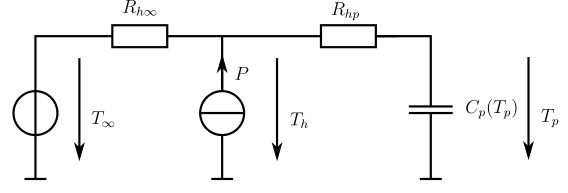
\includegraphics[width=12.5cm]{tikz/2_10_15_1b}
\end{figure}
\newline
Relevanten Größen:
\begin{align*}
	R_{h\infty} = \frac{1}{2r_o\pi L \alpha_\infty} \\
	C_p = r^2_i \pi L \rho_p c_{p,p}(T)
\end{align*}
und
\[
	R_{hp} = \frac{1}{2r_o\pi L k(r_o)}
\]
mit
\[
	k(r) = \frac{1}{r}\frac{1}{\frac{1}{\alpha_{hz}r_o} + \frac{1}{\lambda_z}\log\left( \frac{r_o}{r_i}\right) + \frac{1}{\alpha_{zp}r_i}}
\]
$k(r)$ wurde mit der Formel bei einer Wärmeleitung bei mehrschichtigen zylindrischen Wandaufbau aufgestellt.\\ \\
Einheiten:
\begin{align*}
	[R] &= KW^{-1} \\
	[C] &= JK^{-1} \\
	[P] &= W \\
	[T] &= K
\end{align*}
c) \\ \\
Die Differentialgleichung für die Ersatzschaltung lautet
\[
	\underbrace{(R_{hp} + R_{h\infty})C_p(T_p)}_{\tau(T_p)}\dot{T}_p = T_\infty + PR_{h\infty} - T_p
\]
Dadurch das $c_{p,p} = const$, wird die Differentialgleichung zu einer einfachen DGL 1.Ordnung.
Löst man diese erhält man die Lösung
\[
	T_p(t) = T_\infty + PR_{h\infty}(1 - exp(-t / \tau))
\]
	\newpage
\noindent
\textbf{Beispiel 2} \\ \\
a)\\ \\
Der Anteil durch die freie Konvektion lautet
\[
	\alpha_1(T_1)(T_1 - T_\infty)
\]
Mit der thermischen Strahlung  ergibt sich eine Leistung von
\[
	P = 2r_oL(\alpha_1(T_1)(T_1 - T_\infty) + \dot{q}_1)
\]
b) \\ \\
Dadurch das es sich bei den Oberflächen des Zylinders und des Maschinenbettes um konvexe Flächen handelt sind die Sichtfaktoren $F_{11}$ und $F_{22}$ gleich 0. Mit 
\[
	F_{11} + F_{12} + F_{1\infty} = 1
\]
und bekannten $F_{12}$ folgt
\[
	F_{1\infty} = 1 - F_{12}
\]
Aus dem Reziprozitätsgesetz schließt man
\begin{align*}
	CF_{21} = 2r_o\pi F_{12} \\
	F_{21} = \frac{2r_o\pi}{C}F_{12}
\end{align*}
Verwendet man das gleiche Gesetzt noch einmal an kann man daraus schließen das $F_{\infty1}$ und $F_{\infty2}$ gleich 0 ist, da $A_\infty \rightarrow \infty$. Mithilfe der Summationsregel kann man auf den Sichtfaktor $F_{\infty \infty}$ schlussfolgern, welcher den Wert 1 haben muss.\\ \\
c) \\ \\
Nettowärmestromdichte
\[
	\dot{\textbf{q}} = (\textbf{E} - \textbf{F})(\textbf{E} - (\textbf{E} - diag (\varepsilon))\textbf{F})^{-1}diag(\varepsilon)\sigma\textbf{T}^4
\]
mit
\[
	\dot{\textbf{q}} = [\dot{q}_1,\dot{q}_2,\dot{q}_\infty]^T , \textbf{T} = [T_1,T_2,T_\infty]^T, \varepsilon = [\varepsilon_1,\varepsilon_2,\varepsilon_\infty]^T
\]
der Einheitsmatrix \textbf{E} und dadurch das die Halle ein schwarzer Strahler ist, gilt
\[
	\varepsilon_\infty = 1
\]
Die Sichtfaktormatrix lautet
\[
	\textbf{F} = \begin{bmatrix}
	0 & F_{12} & F_{1\infty} \\
	F_{21} & 0 & F_{2\infty} \\
	0 & 0 & F_{\infty \infty}
	\end{bmatrix}
\]
	\newpage
\noindent
\textbf{Beispiel 3} \\ \\
Da für dieses Beispiel keine Musterlösung existiert, konnten leider keine Berechnungen durchgeführt werden, um diese dann anschließend mit der Musterlösung zu vergleichen. \\ \\
	\textbf{Beispiel 4} \\ \\
a) \\ \\
Aus der Zeichnung kann man direkt 
\[
	\textbf{p}_L = \begin{bmatrix}
		s + \sin\varphi \\
		- l \cos\varphi
	\end{bmatrix}
\]
ablesen. Um $\dot{\textbf{p}}_L$ zu bestimmen, muss man $\textbf{p}_L$ nach den Freiheitsgraden $s$ und $\varphi$ ableiten.\\
Geschwindigkeit der Lastposition
\[
	\dot{\textbf{p}}_L = \begin{bmatrix}
		\dot{s} + l\cos\varphi\dot{\varphi} \\
		l\sin\varphi\dot{\varphi}
	\end{bmatrix}
\]
Der Betrag dieses Vektors lautet
\[
	||\dot{\textbf{p}}_L||^2 = \dot{s}^2 + l^2\dot{\varphi}^2 + 2\dot{s}l\dot{\varphi}\cos\varphi
\]
Die kinetische Energie ergibt sich zu
\[
	T = \frac{1}{2} m_K \dot{s}^2 + \frac{1}{2}m_L||\dot{\textbf{p}}_L||^2 + \frac{1}{2} \Theta_{zz}\dot{\varphi}^2
\]
und die potentielle Energie
\[
	V = -m_lgl\cos\varphi + V_0
\]
mit 
\[
	V_0 = m_Lgl
\]
zu
\[
	V = m_Lgl(1 - \cos\varphi) 
\]
b) \\ \\
Um die Bewegungsgleichungen zu bestimmen wird als erstes die Lagrange-Funktion benötigt welche lautet
\begin{align*}
	L &= T - V = \frac{1}{2} m_K \dot{s}^2 + \frac{1}{2}m_L||\dot{\textbf{p}}_L||^2 + \frac{1}{2} \Theta_{zz}\dot{\varphi}^2 - m_Lgl(1 - \cos\varphi) \\
	&=  \frac{1}{2} m_K \dot{s}^2 + \frac{1}{2}m_L (\dot{s}^2 + l^2\dot{\varphi}^2 + 2\dot{s}l\dot{\varphi}\cos\varphi)  + \frac{1}{2} \Theta_{zz}\dot{\varphi}^2 - m_Lgl(1 - \cos\varphi)
\end{align*}
Euler-Lagrange-Formalismus
\[
	\frac{d}{dt}\frac{\partial L}{\partial \dot{\textbf{q}}} - \frac{\partial L}{\partial \textbf{q}} = \textbf{f}_{np}
\]
\newpage
\noindent
Die seperaten Ableitungen
\begin{align*}
	\frac{\partial L}{\partial \textbf{q}} &= \begin{bmatrix}
		0 \\
		-m_Ll\sin\varphi(\dot{s}\dot{\varphi} + g)
	\end{bmatrix}
	\\
	\frac{\partial L}{\partial \dot{\textbf{q}}} &= \begin{bmatrix}
		(m_K + m_L)\dot{s} + m_Ll\dot{\varphi}\cos\varphi \\
		(\Theta_{zz} + m_L)\dot{\varphi} + m_Ll\dot{s}\cos\varphi
	\end{bmatrix}
	\\
	\frac{d}{dt}\frac{\partial L}{\partial \dot{\textbf{q}}} &= \begin{bmatrix}
		(m_k + m_L)\ddot{s} + m_Ll\ddot{\varphi}\cos\varphi - m_Ll\dot{\varphi}^2\sin\varphi \\
		(\Theta_{zz} + m_L)\ddot{\varphi} + m_Ll\ddot{s}\cos\varphi - m_Ll\dot{s}^2\sin\varphi
	\end{bmatrix}
\end{align*}
Die externen Kräfte können direkt aus der Angabe ablesen werden und lauten
\[
	\textbf{f}_{np} = \begin{bmatrix}
		-d_K\dot{s} + F \\ 
		0
	\end{bmatrix}
\]
c) \\ \\
Aus der zweiten Zeile der Bewegungsgleichungen aus Punkt b) erhält man die Bewegungsgleichung der haftenden Laufkatze. Dadurch lautet diese
\[
	(\Theta_{zz} + m_L)\ddot{\varphi} + m_Llg\sin\varphi = 0
\]
d) \\ \\
Als erstes müssen die externen Kräfte um die Haftkraft $F_H$ erweitert werden. Daher lauten diese dann
\[
	\textbf{f}_{np} = \begin{bmatrix}
	-d_K\dot{s} + F + F_H\\ 
	0
	\end{bmatrix}
\]
Betrachtet man laut Hinweis nur die erste Zeile der Bewegungsgleichungen aus Punkt b) mit $\dot{s} = \ddot{s} = 0$ erhält man
\[
	m_Ll\ddot{\varphi}\cos\varphi - m_Ll\dot{\varphi}^2\sin\varphi = F + F_H
\] 
Formt nun auf $F_H$ um und ermittelt man den Betrag erhält man
\[
	|F_H| = |m_Ll\ddot{\varphi}\cos\varphi - m_Ll\dot{\varphi}^2\sin\varphi - F|
\]
Bringt man nun schließlich diese Gleichung auf die Form der Haftreibung erhält man schlussendlich die Haftbedingung
\[
	|F_H| = |m_Ll\ddot{\varphi}\cos\varphi - m_Ll\dot{\varphi}^2\sin\varphi - F| \leq \mu F_N
\]
Mit
\[
	\ddot{\varphi} = - \frac{m_Llg\sin\varphi}{\Theta_{zz} + m_Ll^2}
\]
aus Punkt c), erhält man die vereinfachte Haftbedingung
\begin{align*}
	\biggl|m_Ll\frac{m_Llg\sin\varphi}{\Theta_{zz} + m_Ll^2}\cos\varphi - m_Ll\dot{\varphi}^2\sin\varphi - F\biggl| \leq \mu F_N \\ \\
	\biggl|\frac{gm^2_Ll^2\sin\varphi\cos\varphi}{\Theta_{zz} + m_Ll^2} + m_Ll\dot{\varphi}^2\sin\varphi + F\biggl| \leq \mu F_N
\end{align*}
	
	\newpage
	\subsection{27.11.2015}
	\textbf{Beispiel 1} \\ \\
a)\\ \\
Um das Bremsmoment ermitteln zu können benötigt man zu aller erst einmal die Wirkfläche. In diesem  Beispiel beträgt diese Fläche
\[
	A = \int_{R_i}^{R_a}\int_{0}^{\frac{\pi}{3}}rd\varphi dr = \frac{\pi}{6}\left(R_a^2 - R_i^2\right)
\]
Das Bremsmoment lässt sich mit 
\[
	M_R = \int_{R_i}^{R_a}\int_{0}^{\frac{\pi}{3}} r^2\mu\frac{F_B}{A}d\varphi dr
\]
zu 
\begin{align*}
	M_R &= \int_{R_i}^{R_a}\int_{0}^{\frac{\pi}{3}} r^2\mu F_B \frac{6}{\pi \left(R_a^2 - R_i^2\right)}d\varphi dr = \\
	M_R &= \int_{R_i}^{R_a} r^2 \mu F_B \frac{\cancelto{2}{6}}{\cancel{\pi} \left(R_a^2 - R_i^2\right)} \frac{\cancel{\pi}}{\cancel{3}} dr = \\
	M_R &= \mu F_B \frac{2}{3}\frac{R_a^3 - R_i^3}{R_a^2 - R_i^2}
\end{align*}
Da zwei Bremsbacken zum Abbremsen verwendet werden lautet das gesamte Bremsmoment 
\[
	M_{ges} = 2M_R = \mu F_B \frac{4}{3}\frac{R_a^3 - R_i^3}{R_a^2 - R_i^2}
\]
b) \\ \\
Die Bewegungsdifferenzialgleichung der Schwungscheibe lautet
\[
	\ddot{\varphi} = - \frac{M_{ges}}{\Theta_{zz}}
\]
Das "$-$" vor dem Brauch kommt daher, dass die $\ddot{\varphi}$ mit der Zeit immer kleiner werden soll, da ja ein Bremsvorgang stattfindet.
Die Anfangsbedingungen für dieses Problem lauten
\[
	\varphi(0) = 0
\]
kann aber beliebig gewählt werden, und 
\[
	\omega(0) = \overline{\omega}
\]
\newpage
\noindent
Als nächstes muss man diese Differenzialgleichung lösen. Dies erreicht man durch 2-maliges Integrieren.
\begin{align*}
	\omega(t) = \dot{\varphi}(t) &= - \frac{M_{ges}}{\Theta_{zz}}t + \overline{\omega} \\
	\varphi(t) &= - \frac{M_{ges}}{\Theta_{zz}} \frac{t^2}{2} + \overline{\omega}t
\end{align*}
Damit ergibt sich die Bremsdauer $t_B$ zu
\begin{align*}
	0 &= \overline{\omega} - \frac{M_{ges}}{\Theta_{zz}}t_B \\ 
	\overline{\omega} &= \frac{M_{ges}}{\Theta_{zz}}t_B \\
	t_B &= \frac{\Theta_{zz}\overline{\omega}}{M_{ges}}
\end{align*}
Um die Bremskraft $F_B$ zu bestimmen setzt man $M_{ges}$ ein und formt einfach auf $F_H$ um und man erhält
\[
	F_B = \frac{3}{4}\frac{R_a^2 - R_i^2}{R_a^3 - R_i^3}\frac{\Theta_{zz}\overline{\omega}}{t_B\mu}
\]
c) \\ \\
Die Bremsleistung lässt sich mit $\dot{W}_R = -M_{ges}\omega$ ermitteln. In diesem Fall lautet somit die Bremsleistung
\[
	\dot{W}_R = \frac{M_{ges}^2}{\Theta_{zz}}t - M_{ges}\overline{\omega}
\]
Integriert man nun diese Leistung über die Bremsdauer erhält man die Energie
\begin{align*}
	E_B &= \int_{0}^{t_B}\frac{M_{ges}^2}{\Theta_{zz}}t - M_{ges}\overline{\omega} dt = \\
	&= \frac{1}{2}\frac{M_{ges}^2}{\Theta_{zz}}\frac{\Theta_{zz}^2\overline{\omega}^2}{M_{ges}^2} - M_{ges}\overline{\omega}\frac{\Theta_{zz}\overline{\omega}}{M_{ges}} \\
	&= -\frac{1}{2}\Theta_{zz}\overline{\omega}
\end{align*}
Dies entspricht der im Schwungrad gespeicherten Energie.\\ \\
d) \\ \\
Aus dem ersten Hauptsatz der Thermodynamik ergibt sich die Differenzialgleichung 
\[
	m_Bc_B\frac{dT_B(t)}{dt} = \frac{1}{2}\left(M_{ges}\overline{\omega} - \frac{M_{ges}^2}{\Theta_{zz}}t\right)
\]
Löst man diese Gleichung durch einfaches Integrieren erhält man
\begin{align*}
	T_B(t) = \frac{1}{2m_Bc_B}\left(M_{ges}\overline{\omega}t - \frac{1}{2}\frac{M_{ges}^2}{\Theta_{zz}}t^2\right) + C
\end{align*}
Setzt man die AB $T_B(0) = T_{B,0}$ ein erhält man
\[
	T_B(t) = T_{B,0} + \frac{1}{2m_Bc_B}\left(M_{ges}\overline{\omega}t - \frac{1}{2}\frac{M_{ges}^2}{\Theta_{zz}}t^2\right)
\]
Zum Zeitpunkt $t_B$ ergibt sich nun folgende Temperatur
\begin{align*}
		T_B(t) &= T_{B,0} + \frac{1}{2m_Bc_B}\left(M_{ges}\overline{\omega}t_B - \frac{1}{2}\frac{M_{ges}^2}{\Theta_{zz}}t_B^2\right) = \\
		&= T_{B,0} + \frac{\Theta_{zz}\overline{\omega}^2}{4m_Bc_B} = \\
		&= T_{B,0} - \frac{1}{m_Bc_B}\frac{E_B}{2} 
\end{align*}
	\textbf{Beispiel 2} \\ \\
Die Wärmestromdichte $\dot{q}_{1-\infty}^I$ ohne der Rettungsdecke lässt sich mit der Formel für die Wärmestromdiche bei Konvektion bestimmen. Diese lautet
\[
	\dot{q}_{1-\infty}^I = \varepsilon_1\sigma(T_1^4 - T_\infty^4)
\]
Um den Wärmestrom zu erhalten muss die Wärmestromdichte einfach mit der betreffenden Fläche multipliziert werden.
\[
	Q_{1-\infty}^I = \varepsilon_1A_1\sigma(T_1^4 - T_\infty^4)
\]
Die Sichtfaktormatrix für dieses Wärmeproblem lautet
\begin{align*}
	\textbf{F} = \begin{bmatrix}
		0 & 1 \\
		1 & 0	
	\end{bmatrix}
	\\
	diag(\varepsilon) = \begin{bmatrix}
		\varepsilon_1 & 0 \\
		0 & \varepsilon_2
	\end{bmatrix}
\end{align*}
Mit der Formel für die Nettowärmestromdichte kann der Wärmestrom zwischen den beiden Körpern bestimmt werden zu
\[
	Q_{1-2}^{II} = \sigma A_1 \frac{\varepsilon_1 \varepsilon_2}{\underbrace{1 - (1 - \varepsilon_1)(1 - \varepsilon_2)}_{K}}(T_1^4 - T_2^4 )
\]
Der Wärmestrom zwischen Rettungsdecke und Umgebung lautet
\[
	Q_{2-\infty}^{II} = \varepsilon_2 A_1\sigma(T_2^4 - T_\infty^4)
\]
Da $Q_{1-2}^{II} = Q_{2-\infty}^{II}$ gilt, kann man $T_2^4$ bestimmen zu
\[
	T_2^4 = \frac{K}{K + \varepsilon_2}T_1^4 + \frac{\varepsilon_2}{K + \varepsilon_2}T_\infty^4
\]
Setzt man dies nun in $Q_{1-2}^{II}$ ein erhält man
\[
	Q_{1-2}^{II} = \sigma A_1 \frac{K\varepsilon_2}{K + \varepsilon_2}(T_1^4 - T_\infty^4)
\]
welcher mit $Q_{1-\infty}^{II}$ gleichzusetzen ist.
Nun kann man das Verhältnis zwischen den Wärmeströmen mit und ohne Decke bestimmen und man erhält ein Verhältnis von $2/5$. Daraus kann man schließen, dass durch die Decke $3/5$ weniger Wärme an die Umgebung verloren geht.
	\\ \\
\textbf{Beispiel 3} \\ \\
a)\\ \\
Zur Beschreibung der Bewegung des Schlittens reicht ein einziger Freiheitsgrad aus, da sich sich dieser nur in horizontaler Richtung bewegt. Die geeignete Minimalkoordinate lautet
\[
	q = \varphi_1(t)
\]
b) \\ \\
Die Kniehebelpresse muss folgende Zwangsbedingung erfüllen.
\[
	L_1\sin\varphi_1 - L_2\sin\varphi_2 = 0
\]
Aus dieser kann nun leicht $\varphi_2$ bestimmen.
\begin{align*}
	L_1\sin\varphi_1 - L_2\sin\varphi_2 = 0  \\
	L_2\sin\varphi_2 = L_1\sin\varphi_1 \\
	\varphi_2 = \arcsin\left(\frac{L_1}{L_2}\sin\varphi_1\right)
\end{align*}
c) \\ \\
Die Ortsvektoren können direkt aus der Angabe abgelesen werden.
\begin{align*}
	\textbf{r}_1 &= \frac{L_1}{2}\begin{bmatrix}
		\cos(q) \\
		\sin(q)
	\end{bmatrix} 
	\\
	\textbf{r}_2 &= L_1\begin{bmatrix}
	\cos(q) \\
	\sin(q)
	\end{bmatrix} 
	+ 
	\frac{L_2}{2}\begin{bmatrix}
		\cos(\varphi_2(q)) \\
		-\sin(\varphi_2(q))
	\end{bmatrix}
\end{align*}
d) \\ \\
Die Schwerpunktsgeschwindigkeiten der Schenkel lauten
\begin{align*}
	\textbf{v}_1 &= \frac{L_1}{2}\begin{bmatrix}
		-\sin(q) \\
		 \cos(q)
	\end{bmatrix} \dot{q}
	\\
	\textbf{v}_2 &= L_1 \begin{bmatrix}
	-\sin(q) \\
	\cos(q)
	\end{bmatrix} \dot{q}
	+
	\frac{L_2}{2}\begin{bmatrix}
		-\sin(\varphi_2(q)) \\
		-\cos(\varphi_2(q))
	\end{bmatrix}
	\frac{\partial \varphi_2(q)}{\partial q} \dot{q}
\end{align*}
Die Drehwinkelgeschwindigkeiten lauten
\begin{align*}
	\omega_1 &= \dot{q} \\
	\omega_2 &= - \frac{\partial \varphi_2(q)}{\partial q} \dot{q}
\end{align*}
e) \\ \\
Anfangs müssen einige Zwischenrechnungen durchgeführt werden.
\begin{align*}
	v_1^2 &= \frac{L_1^2}{4}\dot{q}^2(\cos^2(q) + \sin^2(q)) \\
		  &= \frac{L_1^2}{4}\dot{q}^2
\end{align*}
\begin{align*}
	v_2^2 &= \left(-L_1\sin(q)\dot{q} - \frac{L_2}{2}\sin(\varphi_2(q))\frac{\partial \varphi_2(q)}{\partial q}\dot{q}\right)^2 + \left(L_1\cos(q)\dot{q} - \frac{L_2}{2}\cos(\varphi_2(q))\frac{\partial \varphi_2(q)}{\partial q}\dot{q}\right)^2 \\
	&= L_1^2\dot{q}^2\sin^2(q) + L_1L_2\dot{q}^2\sin(q)\sin(\varphi_2(q))\frac{\partial \varphi_2(q)}{\partial q} + \frac{L_2^2}{4}\dot{q}^2\left(\frac{\partial \varphi_2(q)}{\partial q}\right)^2\sin^2(\varphi_2(q)) + \\
	&+ L_1^2\dot{q}^2\cos^2(q) - L_1L_2\dot{q}^2\cos(q)\cos(\varphi_2(q))\frac{\partial \varphi_2(q)}{\partial q} + \frac{L_2^2}{4}\dot{q}^2\left(\frac{\partial \varphi_2(q)}{\partial q}\right)^2\cos^2(\varphi_2(q)) \\
	&= L_1^2\dot{q}^2 + \frac{L_2^2}{4}\dot{q}^2\left(\frac{\partial \varphi_2(q)}{\partial q}\right)^2 - L_1L_2\dot{q}^2\frac{\partial \varphi_2(q)}{\partial q}(\cos(q)\cos(\varphi_2(q)) - \sin(q)\sin(\varphi_2(q))) \\
	&= L_1^2\dot{q}^2 + \frac{L_2^2}{4}\dot{q}^2\left(\frac{\partial \varphi_2(q)}{\partial q}\right)^2 - L_1L_2\dot{q}^2\frac{\partial \varphi_2(q)}{\partial q}\cos(q + \varphi_2(q))
\end{align*}
Die kinetische Energie lässt sich mit den Formeln aus der Formelsammlung bestimmen und lautet daher:
\begin{align*}
	T &= \frac{1}{2} m_1v_1^2 + \frac{1}{2}m_2v_2^2 + \frac{1}{2} \Theta_1 \omega_1^2 + \frac{1}{2}\Theta_2\omega_2^2 \\
	&= \frac{1}{8}m_1L_1^2\dot{q}^2 + \frac{1}{2}m_2L_1^2\dot{q}^2 + \frac{1}{8}m_2L_2^2\left(\frac{\partial \varphi_2(q)}{\partial q}\right)^2\dot{q}^2 - \frac{1}{2}m_2L_1L_2\cos(q + \varphi_2(q))\left(\frac{\partial \varphi_2(q)}{\partial q}\right)\dot{q}^2 + \\
	&+ \frac{1}{2}\Theta_1\dot{q}^2 + \frac{1}{2}\Theta_2\left(\frac{\partial \varphi_2(q)}{\partial q}\dot{q}\right)^2
\end{align*}
f) \\ \\
Die potenzielle Energie der Schenkel zufolge der Schwerkraft lautet
\begin{align*}
	V_q &= \frac{1}{2}m_1gL_1\sin(q) + m_2gL_1\sin(q) - \frac{1}{2}m_2gL_2\sin(\varphi_2(q)) \\
	V_F  &= \frac{1}{2}c_F\left(L_1\cos(q) + \frac{1}{2}L_2\cos(\varphi_2(q)) - x_{F,0}\right)^2
\end{align*}
\newpage
\noindent
g) \\ \\
Angriffspunkte der beiden externen Kräfte:
\begin{align*}
	\textbf{r}_F &= L_1\begin{bmatrix}
		\cos(q) \\
		\sin(q)
	\end{bmatrix}
	\\
	\textbf{r}_{F_L} &= L_1\begin{bmatrix}
	\cos(q) \\
	\sin(q)
	\end{bmatrix}
	+
	L_2 \begin{bmatrix}
		\cos(\varphi_2(q)) \\
		-\sin(\varphi_2(q))
	\end{bmatrix}
\end{align*}
Deren Ableitungen nach der generalisierten Koordinate lautet
\begin{align*}
	\frac{\partial \textbf{r}_F}{\partial q} &= L_1 \begin{bmatrix}
		-\sin(q) \\
		\cos(q)
	\end{bmatrix}
	\\
	\frac{\partial \textbf{r}_{F_L}}{\partial q} &= L_1\begin{bmatrix}
	-\sin(q) \\
	\cos(q)
	\end{bmatrix}
	+
	L_2\begin{bmatrix}
	-\sin(\varphi_2(q)) \\
	-\cos(\varphi_2(q))
	\end{bmatrix}
	\frac{\partial \varphi_2(q)}{\partial q}
\end{align*}
Die Vektoren der externen Kräfte lauten hier
\begin{align*}
	\textbf{F} &= \begin{bmatrix}
	0 \\
	- F
	\end{bmatrix}
	\\
	\textbf{F}_L &= \begin{bmatrix}
		-F_L \\
		0
	\end{bmatrix}
\end{align*}
Mit der Formel für die generalisierten Kräfte aus der Formelsammlung diese folgendermaßen aussehen.
\begin{align*}
	f_F &= \textbf{F}^T\frac{\partial \textbf{r}_F}{\partial q} = -FL_1\cos(q) \\
	f_{F_L} &= \textbf{F}_L^T \frac{\partial \textbf{r}_{F_L}}{\partial q} = F_L \left(L_1\sin(q) + L_2\sin(\varphi_2(q))\frac{\partial \varphi_2(q)}{\partial q}\right)
\end{align*}
	
	\newpage
	\subsection{05.02.2016}
	\textbf{Beispiel 1} \\ \\
Bei diesen Beispiel muss man den physikalischen Hintergrund von Seilrollen genau beachten. \\ \\
a)\\ \\
Um die kinetische Energie T zu bestimmen, benötigt man sämtliche im System auftretenden Geschwindigkeiten.
\begin{align*}
	\omega_{R_1} &= \frac{v}{r_1} \\
	v_{R_2} &= v \frac{r_1}{2r_2} \\
	\omega_{R_2} &= v\frac{r_1}{2r_2^2}
\end{align*}
Somit ergibt sich die kinetische Energie zu
\[
	T = \frac{m_Lv^2}{2} + \frac{\Theta_1\omega_{R_1}^2}{2} + \frac{\Theta_2\omega_{R_2}^2}{2} + \frac{m_2v_{R_2}^2}{2}
\]
b) \\ \\
Die Energie 
\[
	W = F \cdot s
\]
die beim Verschieben benötigt wird lautet
\[
	W = \mu_cm_Lg\cos\phi s
\]
c) \\ \\
Zum Zeitpunkt $t_0$ soll
\[
	V(t_0) = 0
\]
gültig sein.
Zum Zeitpunkt $t_1$ sieht die potentielle Energie folgendermaßen aus
\[
	V(t_1) = m_Lgs\sin\phi - m_2g\frac{r_1}{2r_2}
\]
d) \\ \\
Die aufzuwendende Arbeit durch die Kraft $\textbf{F}$ lautet
\[
	W = Fs\frac{r_1}{2r_2}
\]
e) \\ \\
Aus der Energieerhaltung ergibt sich
\[
	T(t_0) + V(t_0) + W_F - W = T(t_1) + V(t_1)
\]
Bei den Termen mit $t_0$ müssen für $v$ und $\omega$, $v_0$ und $\omega(t_0)$ und bei $t_1$, $v_1$ und $\omega(t_1)$ eingesetzt werden. Schreibt man nun die obige Gleichung komplett aus und formt dieses dann auf die gesuchte Kraft um erhält man
\begin{align*}
	F &=  \frac{2r_2}{sr_1}\left( m_L\frac{v_1^2 - v_0^2}{2} + \Theta_1 \frac{\omega_{R_1}(t_1)^2 - \omega_{R_1}(t_0)^2}{2} + \Theta_2 \frac{\omega_{R_2}(t_1)^2 - \omega_{R_2}(t_0)^2}{2}\right) + \\
	&+\frac{2r_2}{sr_1}  \left(m_2\frac{v_{R_2}(t_1)^2 - v_{R_2}(t_0)^2}{2} + m_Lgs(\sin\phi + \mu_c\cos\phi) - m_2gs\frac{r_1}{2r_2}\right)
\end{align*}
	\textbf{Beispiel 2} \\ \\
a)\\ \\
Die einzelnen Koordinaten der Position des Stabschwerpunktes können direkt aus der Angabe abgelesen werden und lauten daher
\begin{align*}
	x_s &= r\cos\alpha + l_s\sin\beta \\
	y_s &= r\sin\alpha - l_s\cos\beta
\end{align*}
Dessen Ableitungen lauten
\begin{align*}
	\dot{x}_s &= -r\dot{\alpha}\sin\alpha + l_s\dot{\beta}\cos\beta \\
	\dot{y}_s &= r\dot{\alpha}\cos(\alpha) + l_s\dot{\beta}\sin\beta
\end{align*}
b) \\ \\
Anfangs werden die beiden abgeleiteten Koordinaten zu einem Vektor zusammengefasst.
\[
	\textbf{v}_s = \begin{bmatrix}
		-r\dot{\alpha}\sin\alpha + l_s\dot{\beta}\cos\beta \\
		r\dot{\alpha}\cos(\alpha) + l_s\dot{\beta}\sin\beta
	\end{bmatrix}
\]
Bevor nun aber die kinetische Energie des Systems bestimmt werden kann muss aber vorher noch ein kleine Zwischenrechnung durchgeführt werden.
\begin{align*}
	v_s^2 &= \textbf{v}_s^T\textbf{v}_s \\
		  &= (-r\dot{\alpha}\sin\alpha + l_s\dot{\beta}\cos\beta)^2 + (r\dot{\alpha}\cos(\alpha) + l_s\dot{\beta}\sin\beta)^2 \\
		  &= r^2\dot{\alpha}^2\sin^2\alpha - 2rl_s\dot{\alpha}\dot{\beta}\sin\alpha\sin\beta + l_s^2\dot{\beta}^2\cos^2\beta + \\
		  &+ r^2\dot{\alpha}^2\cos^2\alpha + 2rl_s\dot{\alpha}\dot{\beta}\cos\alpha\cos\beta + l_s^2\dot{\beta}^2\sin^2\beta \\
		  &= r^2\dot{\alpha}^2 + l_s^2\dot{\beta}^2 - 2rl_s\dot{\alpha}\dot{\beta}(\sin\alpha\sin\beta - \cos\alpha\cos\beta) \\
		  &= r^2\dot{\alpha}^2 + l_s^2\dot{\beta}^2 - 2rl_s\dot{\alpha}\dot{\beta}\sin(\alpha - \beta)
\end{align*}
Die kinetische Energie hier lautet
\begin{align*}
	T &= \frac{1}{2}m_sv_s^2 + \frac{1}{2}\Theta_T\dot{\alpha} + \frac{1}{2}\Theta_s\dot{\beta} + \frac{1}{2}m_L(r\dot{\alpha} + \dot{l}_c)
\end{align*}
Der letzte Klammerausdruck setzt sich aus der Rotationsgeschwindigkeit $r\dot{\alpha}$ und der Translationsgeschwindigkeit $\dot{l}_c$ zusammen.
\newpage
\noindent
c) \\ \\
Die potentielle Energie setzt sich aus 2 Komponenten zusammen, die Energie bezüglich der Gewichtskraft
\[
	V_g = m_Lg(c - l_c - r\alpha) + m_sgy_s
\]
mit der wählbaren Länge $c$ und der in den Federn gespeicherten Energie
\[
	V_f = c_1\frac{(\beta - \alpha)^2}{2} + c_2 \frac{(l_c - l_{c,0})^2}{2}
\]
Die Summe der beiden ergibt die gesamte potentielle Energie
\begin{align*}
	V &= V_g + V_f \\
	  &= m_Lg(c - l_c - r\alpha) + m_sgy_s + c_1\frac{(\beta - \alpha)^2}{2} + c_2 \frac{(l_c - l_{c,0})^2}{2}
\end{align*}
d) \\ \\
Die einzige externe Kraft ist jene Kraft $F_e$, die an der Last angreift. Der Vektor zum Angriffspunkt dieser Kraft lautet
\[
	\textbf{p}_f = \begin{bmatrix}
		-r \\
		-r\alpha - l_c - c
	\end{bmatrix}
\]
Dessen Ableitungen nach den gewünschten generalisierten Koordinaten lauten
\begin{align*}
	\frac{\partial \textbf{p}_f}{\partial \alpha} &= \begin{bmatrix}
		0 \\
		-r
	\end{bmatrix}
	\\
	\frac{\partial \textbf{p}_f}{\partial \beta} &= \begin{bmatrix}
		0 \\
		0
	\end{bmatrix}
	\\
	\frac{\partial \textbf{p}_f}{\partial l_c} &= \begin{bmatrix}
		0 \\
		-1
	\end{bmatrix}
\end{align*}
Mit dem Vektor
\[
	\textbf{F}_e = \begin{bmatrix}
		0 \\
		-F_e
	\end{bmatrix}
\]
kann mit der Formel
\[
	\tau = \textbf{F}^T \frac{\partial \textbf{p}}{\partial \textbf{q}}
\]
die generalisierten Kräfte bestimmt werden.
Diese lauten
\begin{align*}
	\tau_\alpha &= rF_e \\
	\tau_\beta &= 0 \\
	\tau_{l_c} &= F_e
\end{align*}
\newpage
\noindent
e) \\ \\
Die Lagrange-Funktion sieht hier folgendermaßen aus.
\begin{align*}
	L &= T - V \\
	  &= \frac{1}{2}m_sv_s^2 + \frac{1}{2}\Theta_T\dot{\alpha} + \frac{1}{2}\Theta_s\dot{\beta} + \frac{1}{2}m_L(r\dot{\alpha} + \dot{l}_c) - \\
	  &- m_Lg(c - l_c - r\alpha) - m_sgy_s - c_1\frac{(\beta - \alpha)^2}{2} - c_2 \frac{(l_c - l_{c,0})^2}{2}
\end{align*}
Die Euler-Lagrange-Gleichungen lauten daher hier
\begin{align*}
	\frac{d}{dt}\left(\frac{\partial L}{\partial \dot{\alpha}}\right) - \frac{\partial L}{\partial \alpha} &= \tau_\alpha \\
	\frac{d}{dt}\left(\frac{\partial L}{\partial \dot{\beta}}\right) - \frac{\partial L}{\partial \beta} &= \tau_\beta \\
	\frac{d}{dt}\left(\frac{\partial L}{\partial \dot{l}_c}\right) - \frac{\partial L}{\partial l_c} &= \tau_{l_c}
\end{align*}
	\textbf{Beispiel 3} \\ \\
a)\\ \\
Das physikalische Prinzip, welches die Wärmeübertragung bestimmt heißt erzwungene Konvektion. Hierbei handelt es sich um eine Randbedingung dritter Art, also eine gemischte Randbedingung. \\ \\ 
b) \\ \\
Das RC-Ersatzbild sieht wie folgt aus
\begin{figure}[h]
	\centering
	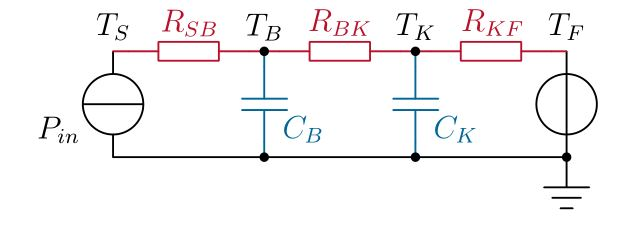
\includegraphics[width=10cm]{tikz/05_02_2016_3b}
\end{figure}
\newline
Die einzelnen Größen werden zu
\begin{align*}
	P_{in} &= I_a(U_e - U_a) \\
	R_{SB} &= aus dem Datenblatt \\
	C_B &= m_Bc_B \\
	R_{BK} &= \frac{h_p}{\lambda_p A_p} \\
	C_K = m_Kc_K &= \rho_K l_K b_k h_K c_K
\end{align*}
\newpage
\noindent
c) \\ \\ 
Ausgangspunkt sind die zur Ersatzschaltung zugehörigen Knoten- und Maschengleichungen
\begin{align*}
	sC_BT_B &= \dot{Q}_{SB} - \dot{Q}_P \\
	sC_KT_K &= \dot{Q}_P - \dot{Q}_{KF} \\
	R_{KF}\dot{Q}_{KF} &= T_K - T_F \\
	\dot{Q}_PR_{BK} &= T_B - T_K \\
	\dot{Q}_{SB}R_{SB} &= T_S - T_B \\
	\dot{Q}_{SB} &= P_{in}
\end{align*}
Löst man dieses Gleichungssystem nach $\dot{Q}_P$ erhält man
\[
	\dot{Q}_P = \frac{(C_KR_{KF}s + 1)P_{in} - C_BT_Fs}{(C_BC_KR_{BK}R_{KF}s^2 + (C_BR_{BK} + C_BR_{KF} + C_KR_{KF}) + 1)}
\]
Im stationären Fall gilt
\[
	\dot{Q}_P = P_{in}
\]
d) \\ \\
Aus der stationären Lösung aus Punkt c) folgt
\[
	P_{in} = \frac{T_S - T_F}{R_{SB} + R_{BK} + R_{KF}}
\]
somit darf der gefragte Widerstand nicht den Wert
\[
	R_{KF,max} \leq \frac{T_{S,max} - T_F}{P_{in}} - R_{SB} -R_{BK}
\]
nicht überschreiten, damit die Temperatur $T_{S,max}$ stationär nicht überschreitet.
	
	\newpage
	\subsection{11.03.2016}
	\textbf{Beispiel 1} \\ \\
a) \\ \\
Bei diesem Messversuch treten Haftreibung
\[
	f_H = \mu_Hmg
\]
trockene Gleitreibung
\[
	f_C = \mu_C m g \, \text{sign}\dot{x}
\]
und viskose Reibung
\[
	f_r = \mu_V \Delta v
\]
auf.
Im folgenden werden diese drei Fälle unterschieden
\[
	f_e = \begin{cases}
		f_H & \text{für} \, \dot{x} = 0 \\
		f_C + f_r & \text{sonst}
	\end{cases}
\]
b) \\ \\
Reibparameter:
\begin{align*}
	\mu_H &= \frac{f_H}{mg} = \frac{0.1 N}{1kgms^{-2}} = 0.1 \\
	\mu_C &= \frac{f_C}{mg} = \frac{0.1 N}{1kgms^{-2}} = 0.1 \\
	\mu_V &= \frac{f_r}{\Delta v} = \frac{0.1N}{1ms^{-1}} = 0.1 Nsm^{-1}
\end{align*}
c) \\ \\
\begin{figure}[h]
	\centering
	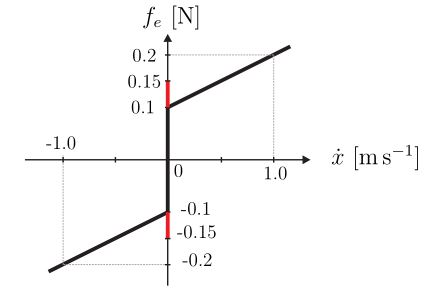
\includegraphics[width=8cm]{tikz/11_03_2016_1c}
\end{figure}
	\newpage
\noindent
\textbf{Beispiel 2} \\ \\
a) \\ \\
Skizze der auftretenden Kräfte
\begin{figure}[h]
	\centering
	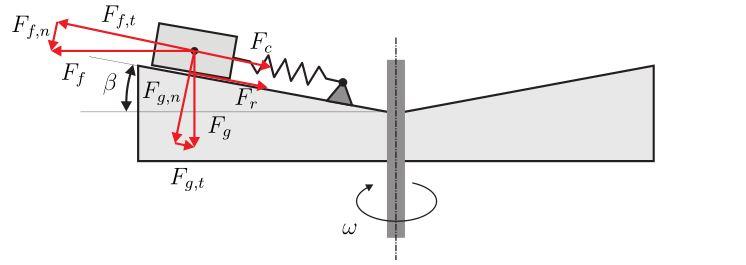
\includegraphics[width=12.5cm]{tikz/11_03_2016_2a}
\end{figure}
\newline
Hier treten die Fliehkraft
\[
	F_f = m(x_m + l)\cos\beta\omega^2
\]
die Gewichtskraft
\[	
	F_g = mg
\]
die Federkraft
\[
	F_c = c (x_m - x_0)
\]
und die Reibkraft (Haftreibung) 
\[
	F_r = (F_{g,n} + F_{f,n})\mu_H
\]
auf. Die einzelnen Terme der Reibkraft werden im nächsten Punkt genauer erklärt.\\ \\
b) \\ \\
Die einzelnen Komponenten der auftretenden Kräfte lauten
\begin{align*}
	F_{f,t} &= m(x_m + l)\cos\beta\omega^2 \\
	F_{f,n} &= m(x_m + l)\cos\beta\sin\beta\omega^2 \\
	F_{g,t} &= mg\sin\beta \\
	F_{g,n} &= mg\cos\beta
\end{align*}
c)\\ \\
Die beiden Haftbedingungen lauten
\begin{align*}
	F_{f,t} - F_{g,t} - F_c &> \mu_H (F_{g,n} + F_{f,n}) \rightarrow \text{Bewegung nach außen} \\
	F_{f,t} - F_{g,t} - F_c &< -\mu_H (F_{g,n} + F_{f,n}) \rightarrow \text{Bewegung nach innen}
\end{align*}
\newpage
\noindent
d) \\ \\ 
Die kritische Winkelgeschwindigkeit kann aus der ersten Haftbedingung wie folgt ermittelt werden.
\begin{align*}
	&F_{f,t} - F_{g,t} - F_c > \mu_H (F_{g,n} + F_{f,n}) \\
	&m(x_m + l)\cos\beta\omega^2 - mg\sin\beta - c(x_m - x_0) > \mu_H (mg\cos\beta + m(x_m + l\cos\beta\sin\beta\omega^2)) \\
	& \omega^2 > \frac{mg\sin\beta + c(x_m - x_0) + \mu_Hmg\cos\beta}{m(x_m + l)\cos\beta - \mu_Hm(x_m + l)\cos\beta\sin\beta} \\
	&\omega > \sqrt{\frac{mg\sin\beta + c(x_m - x_0) + \mu_Hmg\cos\beta}{m(x_m + l)\cos\beta - \mu_Hm(x_m + l)\cos\beta\sin\beta}} \\
	&\omega < - \sqrt{\frac{mg\sin\beta + c(x_m - x_0) + \mu_Hmg\cos\beta}{m(x_m + l)\cos\beta - \mu_Hm(x_m + l)\cos\beta\sin\beta}}
\end{align*} 
	\textbf{Beispiel 3} \\ \\
a) \\ \\
Die hier geeigneten generalisierten Koordinaten sind
\[
	\textbf{q} = \begin{bmatrix}
		\varphi_1 \\
		\varphi_2 \\
		s
	\end{bmatrix}
\]
b)\\ \\
Die kinetische Energie dieses Systems lautet
\[
	T = \frac{1}{2}m_s\dot{s}^2 + \frac{1}{2} \Theta_1 \dot{\varphi_1}^2 + \frac{1}{2} \Theta_2 \dot{\varphi_2}^2
\]
c) \\ \\
Die potentielle Energie dieses Systems lautet
\[
	V = \frac{1}{2} c_1 (s - r\varphi_1)^2 + \frac{1}{2} c_2 (r\varphi_2 - s)^2 + \frac{1}{2} c_3 r^2(\varphi_1 - \varphi_2)^2
\]
d) \\ \\
Um den Euler-Lagrange-Formalimus anwenden zu können benötigt man sowohl die Lagrange-Funktion L und die generalisierten Kräfte. \\
Lagrange-Funktion
\[
	L = T - V = \frac{1}{2}m_s\dot{s}^2 + \frac{1}{2} \Theta_1 \dot{\varphi_1}^2 + \frac{1}{2} \Theta_2 \dot{\varphi_2}^2 - \frac{1}{2} c_1 (s - r\varphi_1)^2 - \frac{1}{2} c_2 (r\varphi_2 - s)^2 - \frac{1}{2} c_3 r^2(\varphi_1 - \varphi_2)^2
\]
Die generalisierten Kräfte können direkt aus der Angabe abgelesen werden.
\[
	f_{np} = \begin{bmatrix}
		M_1 \\
		0 \\
		-\mu_V\dot{s}
	\end{bmatrix}
\]
Euler-Lagrange-Formalimus:
\begin{align*}
	\frac{d}{dt}\left(\frac{\partial L}{\partial \dot{\varphi_1}}\right) - \left(\frac{\partial L}{\partial\varphi_1}\right) &= M_1\\
	\frac{d}{dt}\left(\frac{\partial L}{\partial \dot{\varphi_2}}\right) - \left(\frac{\partial L}{\partial \varphi_2}\right) &= 0\\
	\frac{d}{dt}\left(\frac{\partial L}{\partial \dot{s}}\right) - \left(\frac{\partial L}{\partial s}\right) &= -\mu_V\dot{s}
\end{align*}
Einzelne Ableitungen nach $\textbf{q}$:
\begin{align*}
	\frac{\partial L}{\partial \varphi_1} &= c_1r(s - r\varphi_1) - c_3r^2(\varphi_1 - \varphi_2) \\
	\frac{\partial L}{\partial \varphi_2} &= - c_2r(r\varphi_2 - s) + c_3r^2(\varphi_1 - \varphi_2) \\
	\frac{\partial L}{\partial s} &= -c_1(s - r\varphi_1) + c_2(r\varphi_2 - s)
\end{align*}
Einzelne Ableitungen nach $\dot{\textbf{q}}$:
\begin{align*}
	\frac{\partial L}{\partial \dot{\varphi_1}} &= \Theta_1\dot{\varphi_1} \\
	\frac{\partial L}{\partial \dot{\varphi_2}} &= \Theta_1\dot{\varphi_2} \\
	\frac{\partial L}{\partial \dot{s}} &= m_s\dot{s}
\end{align*}
Deren zeitliche Ableitungen:
\begin{align*}
	\frac{d}{dt}\left(\frac{\partial L}{\partial \dot{\varphi_1}} \right) &= \Theta_1\ddot{\varphi_1} \\
	\frac{d}{dt}\left(\frac{\partial L}{\partial \dot{\varphi_2}} \right) &= \Theta_1\ddot{\varphi_2} \\
	\frac{d}{dt}\left(\frac{\partial L}{\partial \dot{s}} \right) &= m_s\ddot{s}
\end{align*}
Der Euler-Lagrange-Formalismus lautet ausgeschrieben
\begin{align*}
	\Theta_1\ddot{\varphi_1} - c_1r(s - r\varphi_1) + c_3r^2(\varphi_1 - \varphi_2) &= M_1 \\
	\Theta_1\ddot{\varphi_2} + c_2r(r\varphi_2 - s) - c_3r^2(\varphi_1 - \varphi_2) &= 0 \\
	m_s\ddot{s} + c_1(s - r\varphi_1) - c_2(r\varphi_2 - s) &= -\mu_V\dot{s}
\end{align*}
\newpage
\noindent
Somit lauten die Bewegungsgleichungen
\begin{align*}
	\ddot{\varphi_1} &= \frac{1}{\Theta_1}(M_1 + c_1r(s - r\varphi_1) - c_3r^2(\varphi_1 - \varphi_2))\\
	\ddot{\varphi_2} &= \frac{1}{\Theta_2}(-c_2(r\varphi_2 - s) + c_3r^2(\varphi_1 - \varphi_2)) \\
	\ddot{s} &= \frac{1}{m_s}(-c_1(s - r\varphi_1) + c_2(r\varphi_2 - s) - \mu_V\dot{s})
\end{align*}
e) \\ \\
Die Feder 1 ist parallel zu Federn 2 und 3, die Serie zu sehen sind. Daraus folgt eine Gesamtsteifigkeit von
\[
	c = c_1 + \frac{c_2c_3}{c_2 + c_3}
\]
Hier muss nur beachtet werden wie sich Federn verhalten wenn sie in Serie oder parallel verbaut sind. \\ \\
f) \\ \\
Die Bewegungsgleichungen des vereinfachten Systems können anhand der Gleichungen aus Punkt d) leicht bestimmt werden.
\begin{align*}
	\ddot{\varphi_1} &= \frac{1}{\Theta_1}(M_1 + cr(s - r\varphi_1)) \\
	\ddot{s} &= \frac{1}{m_s}(-c(s - r\varphi_1) - \mu_V\dot{s})
\end{align*}
	\textbf{Beispiel 4} \\ \\
a) \\ \\
Da es sich hier um eine Problemstellung handelt die nur vom Radius r abhängt sieht $\Delta$ folgendermaßen aus
\[
	\Delta = \frac{\partial^2}{\partial r^2} + \frac{1}{r}\frac{\partial}{\partial r}
\]
Für den stationären Fall (keine zeitlichen Ableitungen) folgt für die Wärmeleitgleichung
\[
	\frac{\partial^2 T_R}{\partial r^2} + \frac{1}{r}\frac{\partial T_R}{\partial r} = 0
\]
b) \\ \\
Durch die gegebene Substitution erhält man die Gleichung
\[
	f' + \frac{f}{r} = 0
\]
Setzt man nun für $f$ die gegebene Funktion erhält man
\[
	-\frac{c_0}{r^2} + \frac{c_0}{r^2} = 0
\]
Daraus kann man schließen, dass die gegebene Funktion die Wärmeleitgleichung dieses Problems löst, was zu zeigen war. \\ \\
c) \\ \\
Ausgehend von der Differentialgleichung
\[
	\frac{dT_R}{dr} = \frac{c_0}{r}
\]
erhält man die Lösung dieser wie folgt
\begin{align*}
	dT_R &= \frac{c_0}{r}dr\\
	T_R &=  c_0\ln(r) + c_1
\end{align*}
d) \\ \\
Mit den Randbedingungen
\begin{align*}
	T_i &= c_0\ln(r_i) + c_1 \\
	T_a &= c_0\ln(r_a) + c_1
\end{align*}
folgen die Konstanten
\begin{align*}
	T_i - c_0\ln(r_i) &= T_a - c_0\ln(r_a) \\
	T_i - T_a &= c_0 ( \ln(r_i) - \ln(r_a)) \\
	c_0 &= \frac{T_i - T_a}{\ln(\frac{r_i}{r_a})}
\end{align*}
und
\[
	c_1 = T_i - \frac{T_i - T_a}{\ln(\frac{r_i}{r_a})}\ln(r_i)
\]
Mit diesen folgt die Gleichung 
\begin{align*}
	T_R(r) &= \frac{T_i - T_a}{\ln(\frac{r_i}{r_a})}\ln(r) + T_i - \frac{T_i - T_a}{\ln(\frac{r_i}{r_a})}\ln(r_i) \\
	&= T_i + \frac{T_i - T_a}{\ln(\frac{r_i}{r_a})}\ln(\frac{r}{r_i})
\end{align*}
f)\\ \\
Die Wärmestromdichten lauten
\begin{align*}
	\dot{q}_i &= \alpha_i (T_D - T_i) \\
	\dot{q}_a &= \alpha_a (T_a - T_L)
\end{align*}
Über die Fläche A integriert erhalten wir die Wärmeströme
\begin{align*}
	\dot{Q}_i &= \alpha_i A_i (T_D - T_i) \\
	\dot{Q}_a &= \alpha_a A_a (T_a - T_L)
\end{align*}
Der letzte auftretende Wärmestrom lautet
\begin{align*}
	\dot{Q}_\lambda = -\lambda A(r)\frac{dT_r}{dr} = -\lambda 2\pi \cancel{r}L \frac{T_i - T_a}{\ln(\frac{r_i}{r_a})} \frac{\cancel{r_i}}{\cancel{r}}\frac{1}{\cancel{r_i}} = -2\pi\lambda L\frac{T_i - T_a}{\ln(\frac{r_i}{r_a})}
\end{align*}
Diese drei Wärmeströme stehen zueinander mit folgender Beziehung
\[
	\dot{Q}_i = \dot{Q}_a = \dot{Q}_\lambda
\]
	
	\subsection{13.05.2016}
	\textbf{Beispiel 1} \\ \\
a) \\ \\
Der Schwingenwinkel lässt sich folgendermaßen bestimmen
\begin{align*}
	\tan\varphi_S &= \frac{r_K\cos\varphi_K}{h_K + r_K\sin\varphi_K} \\
	\varphi_S &= \arctan\left( \frac{r_K\cos\varphi_K}{h_K + r_K\sin\varphi_K}\right)
\end{align*}
Dessen Ableitung lautet
\begin{align*}
	\dot{\varphi_S} &= \frac{1}{\left( \frac{r_K\cos\varphi_K}{h_K + r_K\sin\varphi_K}\right)^2 + 1} \frac{-r_K\sin\varphi_K(h_K + r_K\sin\varphi_K) - r_K\cos\varphi_K(r_K\cos\varphi_K)}{h_K^2 + 2h_Kr_K\sin\varphi_K + r_K^2\sin^2\varphi_K}\dot{\varphi_K}\\
	&= \frac{1}{\frac{r_K^2\cos^2\varphi_K}{h_K^2 + 2h_Kr_K\sin\varphi_K + r_K^2\sin^2\varphi_K} + 1}\frac{-r_K\sin\varphi_K(h_K + r_K\sin\varphi_K) - r_K\cos\varphi_K(r_K\cos\varphi_K)}{h_K^2 + 2h_Kr_K\sin\varphi_K + r_K^2\sin^2\varphi_K}\dot{\varphi_K} \\
	&= \frac{1}{\frac{r_K^2\cos^2\varphi_K + h_K^2 + 2h_Kr_K\sin\varphi_K + r_K^2\sin^2\varphi_K}{h_K^2 + 2h_Kr_K\sin\varphi_K + r_K^2\sin^2\varphi_K}}\frac{-r_K\sin\varphi_K(h_K + r_K\sin\varphi_K) - r_K\cos\varphi_K(r_K\cos\varphi_K)}{h_K^2 + 2h_Kr_K\sin\varphi_K + r_K^2\sin^2\varphi_K}\dot{\varphi_K} \\
	&= \frac{h_K^2 + 2h_Kr_K\sin\varphi_K + r_K^2\sin^2\varphi_K}{r_K^2\cos^2\varphi_K + h_K^2 + 2h_Kr_K\sin\varphi_K + r_K^2\sin^2\varphi_K}\frac{-r_K\sin\varphi_K(h_K + r_K\sin\varphi_K) - r_K\cos\varphi_K(r_K\cos\varphi_K)}{h_K^2 + 2h_Kr_K\sin\varphi_K + r_K^2\sin^2\varphi_K}\dot{\varphi_K} \\
	&= \frac{-r_K\sin\varphi_K(h_K + r_K\sin\varphi_K) - r_K\cos\varphi_K(r_K\cos\varphi_K)}{r_K^2\cos^2\varphi_K + h_K^2 + 2h_Kr_K\sin\varphi_K + r_K^2\sin^2\varphi_K}\dot{\varphi_K} \\
	&= -\frac{r_K^2 + r_Kh_K\sin\varphi_K}{r_K^2 + 2\sin\varphi_Kr_kh_K + h_K^2}\dot{\varphi_K}\\
	&= -\frac{r_K(r_K + h_K\sin\varphi_K)}{r_K^2 + 2\sin\varphi_Kr_kh_K + h_K^2}\dot{\varphi_K}
\end{align*}
b) \\ \\
Die Länge der Feder beträgt
\[
	l_F = h_s\tan\varphi_S + 2l_{F0}
\]
Der Tangens ist aus der Geometrie der Angabe ersichtlich. \\ \\
c) \\ \\
Den Schwerpunktpunktsvektor kann man hier direkt aus der Angabe ablesen
\[
	\textbf{r}_S = l_S \begin{bmatrix}
		\sin\varphi_S \\
		\cos\varphi_S
	\end{bmatrix},
\]
und der zugehörige Geschwindigkeitsvektor lautet
\[
	\textbf{v}_S = l_s\begin{bmatrix}
		\cos\varphi_S \\
		-\sin\varphi_S
	\end{bmatrix}
	\dot{\varphi_S}
\]
d) \\ \\
Die beiden kinetischen Energie lauten
\begin{align*}
	T_K &= \frac{1}{2} I_K \dot{\varphi_K}^2 \\
	T_S &= \frac{1}{2}I_S\dot{\varphi_S}^2 + \frac{1}{2}m_Sl_S^2\dot{\varphi_S}^2 \\
	    &= \frac{1}{2}(m_S + l_s^2)\dot{\varphi_S}^2
\end{align*}
e)\\ \\
Die beiden potentiellen Energien lauten
\begin{align*}
	V_S &= l_Sm_sg\cos\varphi_S \\
	V_F &= \frac{1}{2}k_F(l_F - l_{F0}) \\
	    &= \frac{1}{2}k_F(h_s\tan\varphi_S + l_{F0})
\end{align*}
f) \\ \\
Die generalisierte Kraft kann direkt aus der Angabe hergeleitet werden
\[
	Q = M_K
\]
g)\\ \\
Die Lagrange-Funktion lautet hier
\begin{align*}
	L &= T - V \\
	  &= \frac{1}{2}\left(I_K +(I_S + m_Sl_S^2)\left( \frac{r_K(r_K + h_K\sin\varphi_K)}{r_K^2 + 2\sin\varphi_Kr_kh_K + h_K^2}\right)^2\right)\dot{\varphi_K}^2 \\
	  &- l_Sm_sg\cos\left( \arctan\left( \frac{r_K\cos\varphi_K}{h_K + r_K\sin\varphi_K}\right)\right) \\
	  &- \frac{1}{2}k_F\left(h_s \frac{r_K\cos\varphi_K}{h_K + r_K\sin\varphi_K} + l_{F0}\right)
\end{align*}
Die Bewegungsgleichung lässt sich mit folgender Formel bestimmen
\[
	\frac{d}{dt}\left(\frac{\partial L}{\partial \dot{\varphi_K}}\right) - \frac{\partial L}{\partial \varphi_K} = Q
\]
	\newpage
\noindent
\textbf{Beispiel 2}\\ \\
a)\\ \\
\begin{figure}[h]
	\centering
	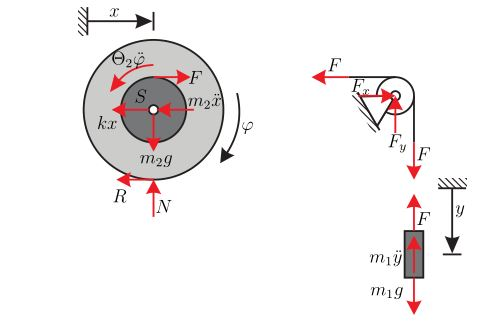
\includegraphics[width=10cm]{tikz/13_05_2016_2a}
\end{figure}
\newline
b)\\ \\
Kräftegleichgewicht der Trommel in der y-Richtung:
\[
	N - m_2g = 0
\]
c)\\ \\
Impuls- und Drehimpulsbilanz der Trommel:
\begin{align*}
	F - R - kx - m_2\ddot{x} &= 0 \\
	r_iF + r_aR - \Theta_2\ddot{\varphi} &= 0
\end{align*}
d) \\ \\
Impulsbilanz des Blockes in y-Richtung:
\[
	m_1g - F - m_1\ddot{y} = 0
\]
e)\\ \\
Da Geschwindigkeit im Punkt M gleich $0$ ist, gilt folgender Zusammenhang für den Schwerpunkt S
\begin{align*}
	\dot{x} &= r_a\dot{\varphi} \\
	\ddot{x} &= r_a\ddot{\varphi}
\end{align*}
\begin{figure}[h]
	\centering
	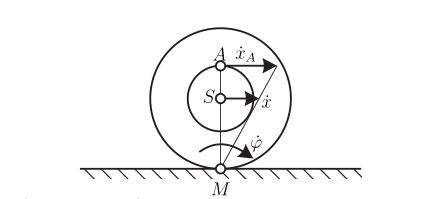
\includegraphics[width=10cm]{tikz/13_05_2016_2e}
\end{figure}
\newpage
\noindent
f)\\ \\
Zusammenhang:
\begin{align*}
	\dot{y} &= (r_i + r_a)\dot{\varphi} \\
	\ddot{y} &= (r_i + r_a)\ddot{\varphi}
\end{align*}
Dieser Zusammenhang ist aber nur dann gültig, wenn das Seil nicht ausgedehnt ist, da in diesem Fall $\dot{y} = \dot{x}_A$ gilt.\\ \\
g)\\ \\
Aus der Impulsbilanz der Trommel folgt
\[
	F = m_2\ddot{x} + R + kx
\]
Setzt man dies in die Drehimpulsbilanz ein und formt diese nach R um, erhält man
\[
	R = \frac{-m_2r_i\ddot{x} + \Theta_2\ddot{x} - kxr_i}{r_i + r_a}
\]
Rückeingesetzt ergibt das 
\[	
	F = m_2\ddot{x} + \frac{-m_2r_i\ddot{x} + \Theta_2\ddot{x} - kxr_i}{r_i + r_a} + kx
\]
Setzt man nun alle bekannten Größen in die Impulsbilanz des Blockes ein, erhält man schließlich
\[
	m_1g - m_2\ddot{x} - \frac{-m_2r_i\ddot{x} + \Theta_2\ddot{x} - kxr_i}{r_i + r_a} - kx - m_1(r_i + r_a)\ddot{\varphi} = 0
\]
Formt man nun diese Gleichung auf $\ddot{\varphi}$ um, ergibt sich
\[
	\ddot{\varphi} = \frac{- m_2\ddot{x}r_a + m_1g(r_i + r_a) - kxr_a}{m_1(r_i + r_a)^2 + \Theta_2}
\]
Dies in $\ddot{x}$ eingesetzt, folgt
\[
	\ddot{x} = \frac{-m_2\ddot{x}r_a^2 + m_1gr_a(r_i + r_a) - kxr_a^2}{m_1(r_i + r_a)^2 + \Theta_2}
\]
Somit folgt die Bewegungsgleichung
\begin{align*}
\ddot{x}\left( 1 + \frac{m_2r_a^2}{m_1(r_i + r_a)^2 + \Theta_2}\right) &= \frac{m_1gr_a(r_i + r_a) - kxr_a^2}{m_1(r_i + r_a)^2 + \Theta_2} \\
\ddot{x}\left(\frac{m_1(r_i + r_a)^2 + \Theta_2 + m_2r_a^2}{m_1(r_i + r_a)^2 + \Theta_2}\right)  &= \frac{m_1gr_a(r_i + r_a) - kxr_a^2}{m_1(r_i + r_a)^2 + \Theta_2} \\
\end{align*}
zu
\[
\ddot{x} = \frac{m_1(r_i + r_a)gr_a - kxr_a^2}{m_1(r_i + r_a)^2 + m_2r_a^2 + \Theta_2}
\]
	\textbf{Beispiel 3}\\ \\
a)\\ \\
Die Wärmeleitgleichungen für das Kabel und die Isolation können mithilfe der Wärmeleitgleichung für Zylinderkoordinaten aus der Formelsammlung aufgestellt werden und daher lauten diese
\begin{align*}
	\rho_l c_l \frac{\partial T_l(r,t)}{\partial t} &= \lambda_l \left(\frac{1}{r}\frac{\partial }{\partial r}\left( r\frac{\partial T_l(r,t)}{\partial r}\right) + \frac{1}{r^2}\frac{\partial^2T_l(r,t)}{\partial \varphi^2} + \frac{\partial^2 T_l(r,t)}{\partial z^2}\right) + g \\
	\rho_i c_i \frac{\partial T_i(r,t)}{\partial t} &= \lambda_i \left(\frac{1}{r}\frac{\partial }{\partial r}\left( r\frac{\partial T_i(r,t)}{\partial r}\right) + \frac{1}{r^2}\frac{\partial^2T_i(r,t)}{\partial \varphi^2} + \frac{\partial^2 T_i(r,t)}{\partial z^2}\right)
\end{align*}
Da es sich um ein unendlich langes Kabel handelt, kann die Abhängigkeit der z-Koordinate vernachlässigt werden. Außerdem kann aufgrund der Kabelsymmetrie die Abhängigkeit von $\varphi$ entfallen. \\
An der Stelle $r = 0$ muss
\[
	\frac{\partial T_l}{\partial r}\biggl|_{r=0} = 0
\]
Die Lösung der Wärmeleitgleichung muss 2-mal stetig differnzierbar sein, daher gilt an der Kontaktstelle $r_i = r_l$
\[
	T_l(r,t) = T_i(r,t)
\]
Mittels Konvektion tauscht das Kabel samt Isolation Wärme mit der Umgebung aus und somit muss an der Stelle $r = r_i$
\[
	-\lambda_i\frac{\partial T_i(r,t)}{\partial r}\biggl|_{r = r_i} = -\dot{q}^a(t)
\]
Die Gleichung wurde mithilfe des Wärmeleitgesetzes aus der Formelsammlung aufgestellt. \\ \\
b)\\ \\
Im stationären Fall verschwindet die zeitlichen Ableitungen, daher erhalten wir die Wärmeleitgleichungen
\begin{align*}
	0 &= \lambda_i\left( \frac{1}{r}\frac{\partial }{\partial r}\left( r\frac{\partial T_l(r,t)}{\partial r}\right)\right) + g \\
	0 &= \frac{\partial }{\partial r}\left( r\frac{\partial T_i(r,t)}{\partial r}\right)
\end{align*}
\newpage
\noindent
Nun folgt die Überprüfung ob die beiden bekannten Temperaturprofile die stationären Gleichungen erfüllen.\\
$T_l(r)$:
\begin{align*}
	0 &= \lambda_i\left( \frac{1}{r}\frac{\partial }{\partial r}\left( r\frac{\partial T_l(r,t)}{\partial r}\right)\right) + g \\
	0 &= \lambda_i\left( \frac{1}{r}\frac{\partial }{\partial r}\left(\frac{-2gr^2}{4\lambda_l}\right)\right) + g \\
	0 &= \cancel{\lambda_i}\left( \frac{1}{\cancel{r}}\frac{-g\cancel{r}}{\cancel{\lambda_l}}\right) + g\\
	0 &= -g + g = 0
\end{align*}
$T_i(r)$:
\begin{align*}
	0 &= \frac{\partial }{\partial r}\left( \cancel{r} (T_1 - T_2)\frac{\cancel{r_i}}{\cancel{r}\ln(r_l/r_i)}\frac{1}{\cancel{r_i}}\right) \\
	0 &= 0
\end{align*}
Somit ist bewiesen, dass die beiden gegebenen Temperaturprofile die stationären Wärmeleitgleichungen erfüllen. \\ \\
c)\\ \\
Der Temperaturverlauf sieht wie folgt aus
\begin{figure}[h]
	\centering
	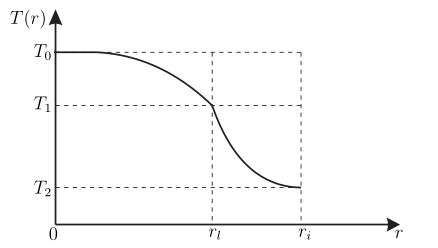
\includegraphics[width=10cm]{tikz/13_05_2016_3c}
\end{figure}
\newline
Unter Berücksichtigung aller Randbedingungen folgt
\[
	T_0 = T_1 + \frac{gr_l^2}{4\lambda_l}
\]
d)\\ \\
Die volumetrische Wärmequelle lautet
\begin{align*}
	g &=  w_l\left(\frac{I}{r_l^2\pi}\right)^2
\end{align*}
Die eingebrachte Energie lautet
\[
	\dot{W} = gr_l^2\pi L = \frac{w_l L}{r_l^2\pi}I^2
\]
e)\\ \\
Die beiden Gesetzmäßigkeiten sind das Reziprozitätsgesetz
\[
	A_iF_{ij} = A_jF_{ji}
\]
und der Summationsregel
\[
	1 = \sum_{j=1}^{N} F_{ij} \qquad \forall \in \{ 1, ... , N\}
\]
Bei konvexen Körpern ist der Sichtfaktor $F_{ii}$ immer gleich 0. \\ \\
f)\\ \\
Die gesuchte Wärmestromdichte wird mithilfe der Nettowärmestromdichte
\[
	\dot{\textbf{q}}_s = (\textbf{E} - \textbf{F})(\textbf{E} - (\textbf{E} - \text{diag}\{\varepsilon\})\textbf{F})^{-1}\text{diag}\{\varepsilon\}\sigma\textbf{T}^4
\]
mit den Vektoren $\dot{\textbf{q}_s} = \left[ \dot{q}_s^a , \dot{q}_s^w\right]^T , \textbf{T} = \left[T_2,T_W\right]^T$ und $\varepsilon = \left[\varepsilon_i , \varepsilon_w\right]^T$ und der Einheitsmatrix
\[
	\textbf{E} = \begin{bmatrix}
		1 & 0 \\
		0 & 1
	\end{bmatrix}
\]
Bestimmung der Sichtfaktoren:
\begin{align*}
	F_{ii} &= 0 \\
	F_{iw} &= 1 \\
	r_i\pi &= (a_w + b_w)F_{wi} \\
	F_{wi} &= \frac{r_i\pi}{a_w + b_w} \\
	F_{ww} &= 1 - \frac{r_i\pi}{a_w + b_w}
\end{align*}
Damit lautet die Sichtfaktormatrix
\[
	\textbf{F} = \begin{bmatrix}
		0 & 1 \\
		\frac{r_i\pi}{a_w + b_w} & 1 - \frac{r_i\pi}{a_w + b_w}
	\end{bmatrix}
\]
g)\\ \\
Die konvektive Wärmestromdichte $\dot{q}_k^a$ lautet
\begin{align*}
	\dot{q}_k^a &= - \alpha(T_2 - T_\infty) \\
				&= \alpha (T_\infty - T_2)
\end{align*}
Somit folgt für den gesamten Wärmestrom $\dot{Q}^a$ an der Stelle $r = r_i$
\[
	\dot{Q}^a = 2r_i\pi L (\dot{q}_k^a +\dot{q}_s^a)
\]
	
	\newpage
	\subsection{08.07.2016}
	\textbf{Beispiel 1}\\ \\
a)\\ \\
Wirkende Kräfte
\begin{figure}[h]
		\centering
		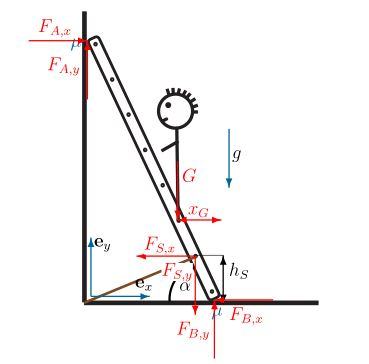
\includegraphics[width=8cm]{tikz/08_07_2016_1a}
\end{figure}
\newline
b)\\ \\
Kräftegleichgewicht:
\begin{align*}
	\textbf{e}_x &: F_{A,x} - F_{B,x} = 0 \\
	\textbf{e}_y &: F_{A,y} + F_{B,y} - G = 0 \quad,G = mg
\end{align*}
Momentengleichgewicht im Fußende der Leiter:
\[
	x_G G - L\cos\alpha F_{A,y} - L\sin\alpha F_{A,x} = 0
\]
c)\\ \\
Die beiden Haftbedingungen lauten 
\begin{align*}
	F_{A,y} &\leq \mu F_{A,x} \\
	F_{B,x} &\leq \mu F_{B,y}
\end{align*}
Setzt man diese in die Gleichungen des Kräftegleichfewichts ein erhält man die Teilkräfte. Anfangs müssen aber noch einige Zwischenrechnungen durchgeführt werden.
\begin{align*}
	F_{A,y} = \mu F_{A,x} &\qquad F_{B,x} = \mu F_{B,y} \\
	F_{A,x} &= F_{B,x} \\
	F_{A,y} &= G - F_{B,y} \\
	\mu F_{A,x} &= G - F_{B,y} \\
	\mu^2 F_{B,y} &= G - F_{B,y} \\
	(\mu^2 + 1) F_{B,y} &= G \\
	F_{B,y} &= \frac{1}{\mu^2 + 1}G \\
	F_{B,x} = F_{A,x} &= \frac{\mu}{\mu^2 + 1} G \\
	F_{A,y} &= \frac{\mu^2}{\mu^2 + 1}
\end{align*}
i)\\ \\
Damit man die Leiter nicht wegrutscht muss
\begin{align*}
	x_G G - L\cos\alpha\frac{\mu^2}{\mu^2 + 1} G - L\sin\alpha\frac{\mu}{\mu^2 + 1} G \leq 0 \\
	x_G \leq L\frac{\mu}{\mu^2 + 1} (\sin\alpha + \mu \cos\alpha)
\end{align*}
ii)\\ \\
Folgende Bedingung gilt für den Steigungswinkel
\[
	\tan\alpha \geq \frac{1}{\mu}
\]
Daraus folgen folgende Grenzen für den Steigungswinkel
\[
	\frac{\pi}{2} \geq \alpha \geq \arctan\left(\frac{1}{\mu}\right)
\]
Aus der Angabe ist ersichtlich das der Steigungswinkel maximal $\frac{\pi}{2}$ sein kann. \\ \\
d)\\ \\
Adaptiertes Kräftegleichgewicht:
\begin{align*}
	F_{A,x} - \mu F_{B,y} - \cos\beta F_S &= 0 \\
	\mu F_{A,x} + F_{B,y} - \sin\beta F_S &= G \\5
	-(L\mu \cos\alpha + L\sin\alpha)F_{A,x} + &\left(\frac{\sin\beta}{\tan\beta} + \cos\beta\right)h_S F_S = -L\cos\alpha G
\end{align*}
\newpage
\noindent
Durch Umformen folgt die Seilkraft
\[
	F_S = G \frac{L\tan\alpha \cos\alpha (\mu^2 + 1)}{((a - h_S(\mu^2 + 1))\cos\beta + a\mu\sin\alpha)\tan\alpha - \sin\beta h_S(\mu^2 + 1)}
\]
mit
\[
	a = L(\sin\alpha + \mu \cos\alpha)
\]
	\textbf{Beispiel 2}\\ \\
a)\\ \\
Der Winkel $\varphi$ und die Position des Zylinder $s_Z$ sind durch ein Rollbewegung miteinander verknüpft. Diese beiden stehen durch 
\[
	\dot{s}_Z - \dot{s}_W = -R\dot{\varphi}
\]
mit den gegebenen generalisierten Koordinaten in Verbindung.\\ \\
b)\\ \\
Schwerpunktsvektoren:
\begin{align*}
	\textbf{r}_W &= s_W\begin{bmatrix}
		\cos\alpha \\
		-\sin\alpha
	\end{bmatrix}
	\\
	\textbf{r}_Z &= s_Z\begin{bmatrix}
	 \cos\alpha \\
	 -\sin\alpha
	\end{bmatrix}
	+
	\left(\frac{h_W}{2} + R\right)\begin{bmatrix}
		\sin\alpha \\
		\cos\alpha
	\end{bmatrix}
\end{align*}
c)\\ \\
Um die kinetische Energie des Gesamtsystemes bestimmen zu können benötigt man zuerst einmal die entsprechenden Geschwindigkeiten.
\begin{align*}
	T_W &= \frac{1}{2}m_W\dot{s}_W^2 \\
	T_Z &= \frac{1}{2}m_Z\dot{s}_Z^2 + \frac{1}{2}\Theta_{zz}\dot{\varphi} \\
		&= \frac{1}{2}m_Z\dot{s}_Z^2 + \frac{1}{2}\frac{\Theta_{zz}}{R^2}(\dot{s}_W - \dot{s}_Z)^2
\end{align*}
Für $\varphi$ wurde die Bedingung aus Punkt a) verwendet.\\ \\
d)\\ \\
Die potentiellen Energien von Wagen und Zylinder lauten
\begin{align*}
	V_W &= -m_W g \sin\alpha s_W \\
	V_Z &= -m_Z g \sin\alpha s_Z
\end{align*}
\newpage
\noindent
e)\\ \\
Die potentiellen Energien der Federn lauten
\begin{align*}
	V_{f1} &= \frac{1}{2} c (l_{f1} - l_0)^2 = \frac{1}{2} c \left(s_W - \frac{l_W}{2} - l_0\right)^2 \\
	V_{f2} &= \frac{1}{2} c (l_{f2} - l_0)^2 = \frac{1}{2} c \left(L - s_W - \frac{l_W}{2} - l_0\right)^2
\end{align*}
f) \\ \\
Zuerst wird einmal die Lagrange-Funktion bestimmt.
\begin{align*}
	L &= T - V = T_W + T_Z - V_W - V_Z - V_{f1} - V_{f2} \\
	  &= \frac{1}{2}m_W\dot{s}_W^2 + \frac{1}{2}m_Z\dot{s}_Z^2 + \frac{1}{2}\frac{\Theta_{zz}}{R^2}(\dot{s}_W - \dot{s}_Z)^2 + m_W g \sin\alpha s_W + m_Z g \sin\alpha s_Z -\\
	  &- \frac{1}{2} c \left(s_W - \frac{l_W}{2} - l_0\right)^2 - \frac{1}{2} c \left(L - s_W - \frac{l_W}{2} - l_0\right)^2
\end{align*}
Euler-Lagrange-Gleichungen:
\begin{align*}
	\frac{d}{dt}\left(\frac{\partial L}{\partial \dot{s}_W}\right) - \frac{\partial L}{\partial s_W} &= 0 \\
	\frac{d}{dt}\left(\frac{\partial L}{\partial \dot{s}_Z}\right) - \frac{\partial L}{\partial s_Z} &= 0
\end{align*}
Einzelne Ableitungen:
\begin{align*}
	\frac{\partial L}{\partial s_W} &= m_W g \sin\alpha - c\left(s_W - \frac{l_W}{2} - l_0\right) + c\left(L - s_W - \frac{l_W}{2} - l_0\right) \\
	&= m_W g \sin\alpha - c(2s_W - L) \\
	\frac{\partial L}{\partial s_Z} &= m_Z g \sin\alpha \\
	\frac{\partial L}{\partial \dot{s}_W} &= m_W \dot{s}_W + \frac{\Theta_{zz}}{R^2}(\dot{s}_W - \dot{s}_Z) \\
	\frac{d}{dt}\left(\frac{\partial L}{\partial \dot{s}_W}\right) &= m_W \ddot{s}_W + \frac{\Theta_{zz}}{R^2}(\ddot{s}_W - \ddot{s}_Z) \\
	\frac{\partial L}{\partial \dot{s}_Z} &= m_Z\dot{s}_Z - \frac{\Theta_{zz}}{R^2}(\dot{s}_W - \dot{s}_Z) \\
	\frac{d}{dt}\left(\frac{\partial L}{\partial \dot{s}_Z}\right) &= m_Z\ddot{s}_Z - \frac{\Theta_{zz}}{R^2}(\ddot{s}_W - \ddot{s}_Z)
\end{align*}
Somit lauten die ausgewerteten Bewegungsgleichungen
\begin{align*}
	 m_W \ddot{s}_W + \frac{\Theta_{zz}}{R^2}(\ddot{s}_W - \ddot{s}_Z) -  m_W g \sin\alpha + c(2s_W - L) &= 0 \\
	 m_Z\ddot{s}_Z - \frac{\Theta_{zz}}{R^2}(\ddot{s}_W - \ddot{s}_Z) -  m_Z g \sin\alpha &= 0
\end{align*}
\newpage
\noindent
Bewegungsgleichungen für die entsprechenden Bereiche
\begin{align*}
	 m_W \ddot{s}_W + \frac{\Theta_{zz}}{R^2}(\ddot{s}_W - \ddot{s}_Z) &= m_W g \sin\alpha - c(2s_W - L) \\
	 m_Z\ddot{s}_Z - \frac{\Theta_{zz}}{R^2}(\ddot{s}_W - \ddot{s}_Z) &=  m_Z g \sin\alpha
\end{align*}
Bereich der ersten Gleichung
\[
	\frac{l_W}{2} \leq s_W \leq L - \frac{l_W}{2}
\]
Bereich der zweiten Gleichung
\[
	s_W - \frac{l_W}{2} + R \leq s_Z \leq s_W + \frac{l_W}{2} - R
\]
	\textbf{Beispiel 3}\\ \\
a)\\ \\
Aufgrund der ebenen Oberflächen strahlen die drei Schienen nicht auf sich selbst ab daher kann man daraus für die Sichtfaktoren
\[
	F_{11} = F_{22} = F_{33} = 0
\]
schließen. Aufgrund der Symmetrie kann man außerdem 
\[
	F_{12} = F_{13} = F_{21} = F_{31} = \overline{F}
\]
sagen.
Aufgrund der gegebenen Anordnung folgt
\[
	F_{23} = F_{32} = 0
\]
Die übrigen Faktoren werden mithilfe der Summationsregel bestimmt. Diese lauten daher
\begin{align*}
	F_{1\infty} &= 1 - 2\overline{F} \\
	F_{2\infty} &= 1 - \overline{F} \\
	F_{3\infty} &= 1 - \overline{F}
\end{align*}
Damit lautet die Sichtfaktormatrix
\begin{align*}
	\textbf{F} = \begin{bmatrix}
		0 & \overline{F} & \overline{F} & 1 - 2\overline{F} \\
		\overline{F} & 0 & 0 & 1 - \overline{F} \\
		\overline{F} & 0 & 0 & 1 - \overline{F} \\
		0 & 0 & 0 & 1
	\end{bmatrix}
\end{align*}
b)\\ \\
Geometrische Zusammenhänge
\begin{align*}
	\sin(\varTheta_{2,0}) &= \frac{L - x}{\sqrt{a^2 + (L - x)^2}} \\
	\sin(\varTheta_{2,1}) &= \frac{2L - x}{\sqrt{a^2 + (2L - x)^2}}
\end{align*}
Nun kann man den Sichtfaktor exakt bestimmen durch
\begin{align*}
	F_{21} &= \frac{1}{2L}\int_{0}^{L} \sin(\varTheta_{2,1}) - \sin(\varTheta_{2,0}) \text{d}x \\
	       &= \frac{1}{2L}\int_{0}^{L} \frac{2L - x}{\sqrt{a^2 + (2L - x)^2}} - \frac{L - x}{\sqrt{a^2 + (L - x)^2}} \\
	       &= \frac{1}{2L}\left(\int_{0}^{L} \frac{2L - x}{\sqrt{a^2 + (2L - x)^2}} \text{d}x - \int_{0}^{L}\frac{L - x}{\sqrt{a^2 + (L - x)^2}}\text{d}x\right)
\end{align*}
Mit der Substitution für das erste Integral 
\begin{align*}
	\sigma &= a^2 + (2L - x)^2 \\
	\text{d}\sigma &= - 2(2L - x) \text{d}x \\
	\text{d}x &= -\frac{\text{d}\sigma}{2(2L - x) }
\end{align*}
und für das zweite Integral
\begin{align*}
	\sigma &= a^2 + (L - x)^2 \\
	\text{d}\sigma &= -2(L - x) \\
	\text{d}x &= -\frac{\text{d}\sigma}{2(L - x)}
\end{align*}
Nun folgt
\begin{align*}
	F_{21} &= \frac{1}{4L}\left( \int_{a^2 + L^2}^{a^2 + 4L^2} \sigma^{-\frac{1}{2}}\text{d}\sigma -  \int_{a^2}^{a^2 + L^2}\sigma^{-\frac{1}{2}}\text{d}\sigma\right) \\
	&= \frac{1}{2L} \left(\sqrt{a^2 + 4L^2} +  a - 2\sqrt{a^2 + L^2}\right)
\end{align*}
c)\\ \\
Aufgrund der Symmetrie folgt 
\[
	A_4 = A_2 + A_3
\]
woraus man 
\[
	\frac{1}{2}A_4 = A_2 = A_3
\]
schließen kann.
Da die Schienen 2 und 3 zu einem Körper zusammengefasst werden, folgt für den Sichtfaktor des zusammengefassten Körper zur Schiene 1
\[
	F_{41} = \overline{F}
\]
Mit dem Reziprozitätsgesetz folgt
\[
	F_{14} = 2\overline{F}
\]
Damit lautet die Sichtfaktormatrix
\[
	\textbf{F} = \begin{bmatrix}
		0 & 2\overline{F} \\
		\overline{F} & 0
	\end{bmatrix}
\]
d)\\ \\
Die Wärmeleitgleichung hier lautet
\[
	\frac{\partial^2}{\partial z^2}T_S(z) = 0
\]
Die Randbedingungen für dieses Wärmeleitproblem lauten
\begin{align*}
	-\lambda\frac{\partial}{\partial z}T_S(0) &= \dot{q}_4 \\
	 T_S(b) &= T_\infty
\end{align*}
Lösungsweg der Wärmeleitgleichung:
\begin{align*}
	\frac{d^2}{d z^2}T_S(z) &= 0 \\
	dT_S(z) &= C_1 dz \\
	T_S(z) &= C_1 z + C_2
\end{align*}
Setzt man nun beide Randbedingungen ein folgt für die Konstanten
\begin{align*}
	C_1 &= -\frac{\dot{q}_4}{\lambda} \\
	C_2 &= T_\infty + \frac{\dot{q}_4}{\lambda}b
\end{align*}
Nun lautet die vollständige Lösung der Wärmeleitgleichung
\[
	T_S(z) = T_\infty + \frac{\dot{q}_4}{\lambda}(b - z)
\]
e)\\ \\
Im stationären Fall müssen sich die Leistungen zu Null bilanzieren. Aus der längenbezogenen Leistungsbilanz für die Schiene 1
\[
	\int_{0}^{L}\dot{q}_1\text{d}x = \int_{0}^{L}\int_{0}^{c}\rho_1\left(\frac{I}{cL}\right)^2\text{d}x\text{d}z
\]
folgt schließlich der Wärmestrom
\[
	\dot{q}_1 = \frac{\rho_1}{cL^2}I^2
\]
Da die Oberflächentemperatur $T_4$ der Schienen 2 und 3 der stationären Lösung am Rand entsprechen muss lautet das nichtlineare Gleichungssystem
\begin{align*}
	\dot{q}_1(T_1,T_4) - \frac{\rho_1}{cL^2}I^2 &= 0 \\
	T_4 - T_\infty - \frac{\dot{q}_4(T_1,T_4)}{\lambda}b &= 0
\end{align*}
Alternativ kann auch die eine Randbedingung aus Punkt d) angepasst werden. Diese lautet damit
\[
	-\lambda\frac{\partial}{\partial z}T_S(0) = \dot{q}_4(T_1,T_4)
\]
	
	\newpage
	\subsection{23.09.2016}
	\textbf{Beispiel 1}\\ \\
a)\\ \\
Mit den Freiheitsgraden
\[
	\textbf{q} = \begin{bmatrix}
		\alpha , \beta , x
	\end{bmatrix}^T
\]
wird das angegebene System vollständig beschrieben.\\ \\
b)\\ \\
Freigeschnittene Körper inklusive aller wirkenden Kräfte:
\begin{figure}[h]
	\centering
	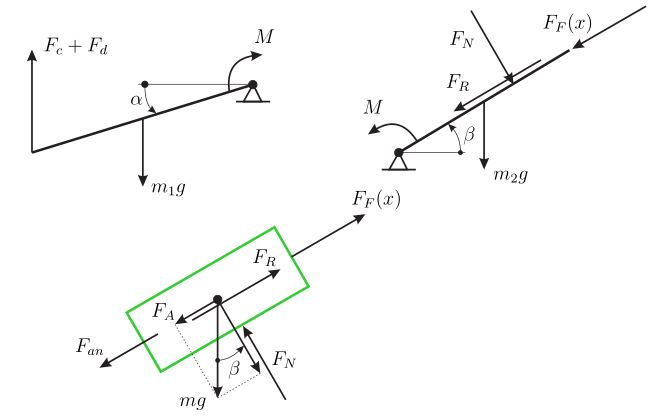
\includegraphics[width= 12cm]{tikz/23_09_2016_1b}
\end{figure}
\newline
Desweiteren gilt:
\begin{align*}
	F_c &= cl_1\sin(\alpha) \\
	F_d &= dl_1\dot{\alpha}\cos(\alpha) \\
	M &= c_D (\alpha - \beta) \\
	F_N &= mg\cos(\beta) \\
	F_A &= mg\sin(\beta)
\end{align*}
Aufgrund der Rotation des Stabes 2 wirkt auch eine Fliehkraft auf die Masse $m$. Diese lautet
\[
	F_{Flieh} = m(l_2 - x)\dot{\beta}^2
\]
c)\\ \\ 
Mit der Form der Haftreibung aus der Formelsammlung folgt die Haftbedingung
\[
	|F_{an} + F_A - F_F(x)| = |F_{an} + mg\sin(\beta) - F_F(x)| \leq mg\cos(\beta)\mu_H
\]
d)\\ \\
Die angegeben Trägheitsmomente bezieht sich jeweils auf die Schwerpunkte der Stäbe. Da sich der Drehpunkt aber am Ende der Stäbe befindet muss man hier den Satz von Steiner anwenden. 
\begin{align*}
	J_1 &= J_{S,1} + m_1\frac{l_1^2}{4} \\
	J_2 &= J_{S,2} + m_2\frac{l_2^2}{4}
\end{align*}
Durch Anwendung des Impuls- und Drallsatz folgen die Bewegungsgleichungen
\begin{align*}
	J_1\ddot{\alpha} &= m_1g\frac{l_1}{2}\cos(\beta) - c_D(\alpha - \beta) - \left(cl_1\sin(\alpha) + dl_1\dot{\alpha}\cos(\alpha)\right)l_1\cos(\alpha) \\
	J_2\ddot{\beta}&= c_D(\alpha - \beta) - m_2g\frac{l_2}{2}\cos(\beta) - mg(l_2 - x)\cos(\beta) \\
	m\ddot{x} &= F_{an} - F_F(x) - \mu_V\dot{x} + mg\sin(\beta)
\end{align*}
Diese Gleichungen können unmittelbar aus den freigeschnittenen Körpern aus Punkt b) abgelesen werden.\\ \\
e)\\ \\
Für sehr kleine Winkel können die Näherungen 
\[
	\sin(\alpha) = \alpha \, , \, \sin(\beta) = \beta
\]
verwendet werden. Daraus kann man 
\[
\cos(\alpha) = 1 \, , \, \cos(\beta) = 1
\]
schließen.\\ \\
f)\\ \\
Nein es ist nicht möglich, weil in dieser Ruhelage die Feder keine Kraft und die Drehfeder kein Moment ausübt. Dadurch können aber nicht die durch die Gewichtskräfte entstehenden Momente ausgeglichen werden können.
	\newpage
\noindent
\textbf{Beispiel 2}\\ \\
a)\\ \\
spezifische Wärmekapazität $c_P$ in $J/(kgK)$ \\
Wärmleitfähigkeit $\lambda$ in $W/(mK)$ \\ \\
b)\\ \\
entsprechende Randbedingungen: \\ 
\begin{align*}
	x &= 0: T(0,t) = T_0 \\
	x &= L: \partial T(L,t)/\partial x = 0 \quad (\text{adiabate Randbedingung zweiter Art})
\end{align*}
c) \\ \\
Die gesuchte Wärmestromdichte kann mittels der Formel für die Wärmestromdichte an der Kontaktfläche zweier Festkörper bestimmt werden.
\[
	\dot{q}_w(T) = \alpha (T_w - T(x,t))
\]
d)\\ \\
i)\\
Der geeignete Zustandsvektor lautet hier
\[
	\textbf{T}(t) = [T_1(t),T_2(t),T_3(t)]^\text{T}
\]
ii)\\
Die Form für die Rückwartsdifferenz und zentrale Differenz kann aus der Formelsammlung entnommen werden. Daher lauten die Rückwärtsdifferenzen
\begin{align*}
	\frac{\partial T(\Delta x,t)}{\partial x} &= \frac{T_1 - T_0}{\Delta x} \\
	\frac{\partial T(i\Delta x,t)}{\partial x} &= \frac{T_i - T_{i-1}}{\Delta x} \quad \text{für} \quad i = 2,3
\end{align*}
und die zentralen Differenzen
\begin{align*}
	\frac{\partial^2 T(i\Delta x,t)}{\partial x^2} &= \frac{(T_{i-1} - 2T_i + T_{i+1})}{\Delta x^2} \quad \text{für} \quad i = 1,2 \\
	\frac{\partial^2 T(L,t)}{\partial x^2} &= \frac{2T_2 - 2T_3}{\Delta x^2}
\end{align*}
\newpage
\noindent
iii)\\
Ersetzt man nun die bisherigen Erkenntnis in die Gleichung aus der Angabe ein erhält man die Gleichungen
\begin{align*}
	\rho c_P \dot{T}_1(t) + \rho c_P \frac{1}{\Delta x}(T_1 - T_0) &= \lambda \frac{1}{\Delta x^2}(T_0 - 2T_1 + T_2) + \frac{4}{d_h}\alpha (T_w - T_1(t)) \\
	\rho c_P \dot{T}_2(t) + \rho c_P \frac{1}{\Delta x}(T_2 - T_1) &= \lambda \frac{1}{\Delta x^2}(T_1 - 2T_2 + T_3) + \frac{4}{d_h}\alpha (T_w - T_2(t)) \\
	\rho c_P \dot{T}_3(t) + \rho c_P \frac{1}{\Delta x}(T_3 - T_2) &= \lambda \frac{1}{\Delta x^2}(2T_2 - 2T_3) + \frac{4}{d_h}\alpha (T_w - T_3(t))
\end{align*}
Vergleicht man nun diese drei Gleichungen mit der Form aus der Angabe erhält man die Matrizen
\begin{align*}
	\textbf{K} &= \frac{1}{\Delta x}\begin{bmatrix}
		1 & 0 & 0 \\
		-1 & 1 & 0 \\
		0 & -1 & 1 
	\end{bmatrix}
	\\
	\textbf{D} &= \frac{1}{\Delta x^2}\begin{bmatrix}
		-2 & 1 & 0 \\
		1 & -2 & 1 \\
		0 & 2 & -2 
	\end{bmatrix}
\end{align*}
und die Vektoren
\begin{align*}
	\textbf{b}_v &= \frac{T_0}{\Delta x}\begin{bmatrix}
		-1 \\
		0 \\
		0
	\end{bmatrix}
	\\
	\textbf{b}_\lambda &= \frac{T_0}{\Delta x^2}\begin{bmatrix}
		1 \\
		0 \\
		0
	\end{bmatrix}
	\\
	\dot{\textbf{q}}_w(\textbf{T}) &= \alpha (T_w\textbf{\text{1}} - \textbf{T})
\end{align*}
e) \\ \\
Durch lösen der Differentialgleichung (1) aus der Angabe erhält man unter Beachtung der Stationärität und den Randbedingungen die folgende Lösung
\[
	T(x) = (T_0 - T_w)exp\left(-\frac{4\alpha}{\rho c_P v d_h}x\right) + T_w
\]
	\newpage
\noindent
\textbf{Beispiel 3}\\ \\
a)\\ \\
Man kann das System noch mit dem Vektor $\textbf{q} = [x_W , x_{1L} , y_{1L}]^T$ beschrieben werden. Die letzten beiden Koordinaten sind die Koordinaten des Lastschwerpunktes bezogen auf das Inertialsystem. Ein weiteres Beispiel wäre $\textbf{q} =[x_w , \alpha , l]^T$, wobei $l$ die abgewickelte Seillänge ist.
b)\\ \\
Die erforderlichen Ortsvektoren sind jene die vom Ursprung des Inertialsystem zu den Schwerpunkten der einzelnen Teile zeigen.
\begin{align*}
	\textbf{r}_W &= \begin{bmatrix}
		x_W \\
		0 \\
		0
	\end{bmatrix}
	\\
	\textbf{r}_L &= \begin{bmatrix}
		x_W - d_0 - d_1 + x_L - (l_0 + r_T\varphi)\sin(\alpha) \\
		-y_L - (l_0 + r_T\varphi)\cos(\alpha) \\
		0
	\end{bmatrix}
\end{align*}
c)\\ \\
Die relevanten Geschwindigkeitsvektoren und Winkelgeschwindigkeitsvektor lauten
\begin{align*}
	\dot{\textbf{r}}_W &= \begin{bmatrix}
		\dot{x}_W \\
		0 \\
		0
	\end{bmatrix}
	\\
	\dot{\textbf{r}}_L &= \begin{bmatrix}
		\dot{x}_W - r_T\dot{\varphi}\sin(\alpha) - (l_0 + r_T\varphi)\cos(\alpha)\dot{\alpha} \\
		-r_T\dot{\varphi}\cos(\alpha) + (l_0 + r_T\varphi)\sin(\alpha)\dot{\alpha} \\
		0
	\end{bmatrix}
	\\
	\omega_T &= \begin{bmatrix}
	 	0 \\
	 	0 \\
	 	\dot{\varphi}
	\end{bmatrix}
\end{align*}
Die kinetische Energien der einzelnen Teile lauten
\begin{align*}
	T_W &= \frac{1}{2}m_W\dot{x}^2_W \\
	T_T &= \frac{1}{2}J_T\dot{\varphi}^2 \\
	T_L &= \frac{1}{2}m_L ((	\dot{x}_W - r_T\dot{\varphi}\sin(\alpha) - (l_0 + r_T\varphi)\cos(\alpha)\dot{\alpha})^2 \\
	&+ (	-r_T\dot{\varphi}\cos(\alpha) + (l_0 + r_T\varphi)\sin(\alpha)\dot{\alpha})^2)
\end{align*}
Die gesamte kinetische Energie des Systems lautet
\[
	T_{ges} = T_W + T_T + T_L
\]
\newpage
\noindent
d)\\ \\
Die potentiellen Einzelenergien lauten
\begin{align*}
	V_W &= 0 \\
	V_L &= -m_L g (y_L + (l_0 + r_T\varphi)\cos(\alpha))
\end{align*}
Die potentielle Energie des Wagens ist 0, weil sich der Wagen immer in derselben Ebene befindet. Die gesamte potentielle Energie des Systems lautet
\[
	V_{ges} = V_L
\]
e)\\ \\
Der Vektor der generalisierten Kräfte kann unmittelbar aus Angabe bestimmt werden, da jede externe Kraft bzw. Moment unmittelbar auf der entsprechenden generalisierten Koordinate wirkt. Der Vektor lautet daher
\[
	\tau = \begin{bmatrix}
		F_{an} - F_R \\
		0 \\
		M_T
	\end{bmatrix}
\]
f)\\ \\
Die Lagrange-Funlktion lautet
\[
	L = T_{ges} - V_{ges}
\]
und damit die Euler-Lagrange-Gleichungen
\[
	\frac{\partial}{\partial t} \left( \frac{\partial L}{\partial \dot{\textbf{q}}}\right) - \frac{\partial L}{\partial \textbf{q}} =  \tau
\]
	
	\newpage
	\subsection{18.11.2016}
	\textbf{Beispiel 1}\\ \\
a)\\ \\
Die gesuchte Zwangsbedingung kann hier unmittelbar aus der Angabe abgelesen werden. Mithilfe der Annahme $f(\varTheta, \psi) = 0$ folgt die Zwangsbedingung
\[
	f(\varTheta, \psi) = L \sin(\varTheta) - L \sin(\varTheta_0) - r\cos(\psi)=0
\]
b)\\ \\
Die beiden gesuchten Ortsvektoren zu den Schwerpunkten der beiden Massen lauten
\[
	\textbf{r}_M = \begin{bmatrix}
		l\cos(\varTheta) - h\sin(\phi) \\
		0 \\
		-l\sin(\varTheta) - h\cos(\psi)
	\end{bmatrix}
\]
und
\[
	\textbf{r}_m = \begin{bmatrix}
		-L\cos(\varTheta) - r\sin(\psi) \\
		0 \\
		L\sin(\varTheta) - r\cos(\psi)
	\end{bmatrix}
\]
b)\\ \\
Die gesuchten Geschwindigkeitsvektoren erhält man wie sonst, durch die zeitliche Ableitung der entsprechenden Ortsvektoren. Daher lauten dieses nun hier
\begin{align*}
	\textbf{v}_M &= \begin{bmatrix}
		-l\sin(\varTheta)\dot{\varTheta} - h\cos(\phi)\dot{\phi} \\
		0 \\
		-l\cos(\varTheta)\dot{\varTheta} + h\sin(\phi)\dot{\phi}
	\end{bmatrix}
\end{align*}
Die Geschwindigkeit der kleinen Masse $m$ muss in den Vektor
\[
	\textbf{v}_{m,1} = \begin{bmatrix}
		L\sin(\varTheta)\dot{\varTheta} - r\cos(\psi)\dot{\psi} \\
		0 \\
		0
	\end{bmatrix}
\]
und in den Vektor
\[
	\textbf{v}_{m,2} = \begin{bmatrix}
		L\sin(\varTheta)\dot{\varTheta} - r\cos(\psi)\dot{\psi} \\
		0 \\
		L\cos(\varTheta)\dot{\varTheta} + r\sin(\psi)\dot{\psi}
	\end{bmatrix}
\]
aufgeteilt werden. Der erste Vektor kann sich nur in der x-Richtung ausbreiten, da sich die Masse $m$ zu dieser Zeit in der Rille befindet. Sobald die kleinen Masse aber diese verlässt, beschreibt nun der zweite Vektor die Geschwindigkeit der Masse $m$.
\newpage
\noindent
d) \\ \\
Bevor die kinetischen Energien bestimmt werden können, müssen zuerst wieder einmal Nebenrechnungen durchgeführt werden.
\begin{align*}
	\textbf{v}_M^T \textbf{v}_M &= (-l\sin(\varTheta)\dot{\varTheta} - h\cos(\phi)\dot{\phi})^2 + (-l\cos(\varTheta)\dot{\varTheta} + h\sin(\phi)\dot{\phi})^2 \\
	&= l^2\dot{\varTheta}^2\sin^2(\varTheta) + 2 l h \dot{\varTheta}\dot{\phi}\sin(\varTheta)\cos(\psi) + h^2\dot{\phi}^2\cos^2(\phi) + l^2\dot{\varTheta}^2\cos^2(\varTheta) - 2 l h \dot{\varTheta}\dot{\phi}\cos(\varTheta)\sin(\phi) + h^2\dot{\phi}^2\sin^2(\phi) \\
	&= l^2\dot{\varTheta}^2(\sin^2(\varTheta) + \cos^2(\varTheta)) + h^2\dot{\phi}^2(\cos^2(\phi) + \sin^2(\phi)) + 2lh\dot{\varTheta}\dot{\phi} (\sin(\varTheta)\cos(\phi) - \cos(\varTheta)\sin(\phi)) \\
	&= l^2\dot{\varTheta}^2 + h^2\dot{\phi}^2 + 2lh\dot{\varTheta}\dot{\phi}\sin(\varTheta - \phi) \\
	\textbf{v}_{m,1}^T\textbf{v}_{m,1} &= (	L\sin(\varTheta)\dot{\varTheta} - r\cos(\psi)\dot{\psi})^2 \\
	\textbf{v}_{m,2}^T\textbf{v}_{m,2} &= (	L\sin(\varTheta)\dot{\varTheta} - r\cos(\psi)\dot{\psi})^2 + (L\cos(\varTheta)\dot{\varTheta} + r\sin(\psi)\dot{\psi})^2 \\
	&= L^2\dot{\varTheta}^2\sin^2(\varTheta) - 2Lr\dot{\varTheta}\dot{\psi}\sin(\varTheta)\cos(\psi) + r^2\dot{\psi}^2\cos^2(\psi) + L^2\dot{\varTheta}^2\cos^2(\varTheta) + 2Lr\dot{\varTheta}\dot{\psi}\cos(\varTheta)\sin(\psi) + r^2\dot{\psi}^2\sin^2(\psi) \\
	&= L^2\dot{\varTheta}^2(\sin^2(\varTheta) + \cos^2(\varTheta)) + r^2\dot{\psi}^2(\cos^2(\psi) + \sin^2(\psi)) - 2Lr\dot{\varTheta}\dot{\psi}(\sin(\varTheta)\cos(\psi) - \cos(\varTheta)\sin(\psi)) \\
	&= L^2\dot{\varTheta}^2 + r^2\dot{\psi}^2 - 2Lr\dot{\varTheta}\dot{\psi}\sin(\varTheta - \psi)
\end{align*}
Da man die einzelnen Trägheitsmomente vernachlässigbar sind, muss man daher nur die translatorischen kinetischen Energien des Gesamtsystems bestimmen.
\begin{align*}
	T_1 &= \frac{1}{2}M(l^2\dot{\varTheta}^2 + h^2\dot{\phi}^2 + 2lh\dot{\varTheta}\dot{\phi}\sin(\varTheta - \phi)) + \frac{1}{2}m(	L\sin(\varTheta)\dot{\varTheta} - r\cos(\psi)\dot{\psi})^2 \\
	T_2 &= \frac{1}{2}M(l^2\dot{\varTheta}^2 + h^2\dot{\phi}^2 + 2lh\dot{\varTheta}\dot{\phi}\sin(\varTheta - \phi)) + \frac{1}{2}m(L^2\dot{\varTheta}^2 + r^2\dot{\psi}^2 - 2Lr\dot{\varTheta}\dot{\psi}\sin(\varTheta - \psi))
\end{align*}
e) \\ \\
Die potentiellen Teilenergien des Gesamtsystems lauten
\begin{align*}
	V_M &= Mg(-l\sin(\varTheta) - h\cos(\psi)) \\
	V_m &= mg(L\sin(\varTheta) - r\cos(\psi)) \\
\end{align*}
Daraus folgen die potentiellen Energien der beiden Phasen.
\begin{align*}
	V_1 &= V_M \\
	V_2 &= V_M + V_m
\end{align*}
	\newpage
\noindent
\textbf{Beispiel 2}\\ \\
a) \\ \\
Ersatzfederelement:
\[
	\tilde{c} = \frac{c_3c_4}{c_3 + c_4}
\]
Ersatzdämpferelement:
\[
	\tilde{d} = d_3 + d_4
\]
entspannte Länge der Ersatzfeder:
\[
	\tilde{s}_0 = s_{03} + s_{04}
\]
b) \\ \\
Wendet man den Impulserhaltungssatz auf beide Massen an, erhält man
\[
	m_1\ddot{s}_1 = -m_1 g - c_1(s_1 - s_{01}) - d\dot{s}_1 + c_2(s_2 - s_1 - s_{02}) + d_2(\dot{s}_2 - \dot{s}_1)
\]
und
\[
	m_2\ddot{s} = -m_2 g - c_2(s_2 - s_1 - s_{02}) - d_2(\dot{s}_2 - \dot{s}_1) - \tilde{c}(s_2 - \tilde{s}_0) - \tilde{d}\dot{s}_2 - f_L
\]
c)\\ \\
Zuerst müssen die gerade ermittelten Differentialgleichungen so umgeformt werden, dass diese die gesuchte Form besitzen. Die gesuchte Form lautet
\[
	\textbf{M}\ddot{\textbf{q}} + \textbf{D}\dot{\textbf{q}} + \textbf{C}\textbf{q} = \textbf{k} + \textbf{b}f_L
\]
umgeformte Gleichungen:
\begin{align*}
	m_1\ddot{s}_1 + (d_1 + d_2)\dot{s}_1 - d_2\dot{s}_2 + (c_1 + c_2)s_1 - c_2 s_2 &= -m_1g + c_1s_{01} - c_2s_{02} \\
	m_2\ddot{s}_2 - d_2s_1 + (\tilde{d} + d_2)\dot{s}_2 - c_2s_1 +(c_2 + \tilde{c})s_2 &= -m_2g + \tilde{c}\tilde{s}_0 + c_2s_{02} - f_L
\end{align*}
Hieraus folgt das System
\[
	\underbrace{\begin{bmatrix}
			m_1 & 0 \\
			0 & m_2
		\end{bmatrix}}_{\textbf{M}}\ddot{\textbf{q}}
	+
	\underbrace{\begin{bmatrix}
			d_1 + d_2 & -d_2 \\
			-d_2 & \tilde{d} + d_2
		\end{bmatrix}}_{\textbf{D}} \dot{\textbf{q}}
	+
	\underbrace{\begin{bmatrix}
			c_1 + c_2 & -c_2 \\
			-c_2 & \tilde{c} + c_2
		\end{bmatrix}}_{\textbf{C}}\textbf{q}
	=
	\underbrace{\begin{bmatrix}
			-m_1g + c_1s_{01} - c_2s_{02} \\
			-m_2g + \tilde{c}\tilde{s}_0 + c_2s_{02}
		\end{bmatrix}}_{\textbf{k}}
	+ 
	\underbrace{\begin{bmatrix}
			0 \\
			-1
		\end{bmatrix}}_{\textbf{b}} f_L
\]
d)\\ \\
Im stationären Fall fallen aus den obigen System die zeitlichen Ableitungen weg und die Postion der von $m_2$ beträgt nun $h$. Daraus folgt nun das System
\[
	\underbrace{\begin{bmatrix}
		c_1 + c_2 & -c_2 \\
		-c_2 & \tilde{c} + c_2
		\end{bmatrix}}_{\textbf{C}}
	\begin{bmatrix}
		s_1 \\
		h
	\end{bmatrix}
	=
	\underbrace{\begin{bmatrix}
		-m_1g + c_1s_{01} - c_2s_{02} \\
		-m_2g + \tilde{c}\tilde{s}_0 + c_2s_{02}
		\end{bmatrix}}_{\textbf{k}}
	+ 
	\underbrace{\begin{bmatrix}
		0 \\
		-1
		\end{bmatrix}}_{\textbf{b}} f_L
\]
mit dem Gleichungssystem
\begin{align*}
	(c_1 + c_2)s_1 - c_2 h &= k_1 \\
	-c_2 s_1 + (\tilde{c} + c_2) h &= k_2 - f_L
\end{align*}
\newpage
\noindent
Formt man nun beide Gleichungen um, erhält man schließlich die gesuchten Größen $f_L$ und $s_1$.\\
Erste Gleichung:
\[
	s_1 = \frac{k_1 + c_2 h }{c_1 + c_2}
\]
Zweite Gleichung:
\[
	f_L = k_2 + c_2 s_1 - (\tilde{c} + c_2)h
\]
Nun wird noch $s_1$ eingesetzt und schließlich erhält man dadurch
\[
	f_L = k_2 + \frac{c_2 (k_1 + c_2 h) }{c_1 + c_2} - (\tilde{c} + c_2)h
\]
e) \\ \\
Aufgrund von Abbildung 3 in der Angabe ergibt sich folgende Form der Geschwindigkeit $v(t)$:
\[
	v(t) = \left\{
		\begin{array}{lll}
			\frac{v_{max}}{t_1}t & \text{für} \quad 0 \leq t \leq t_1 \\
			v_{max} & \text{für} \quad t_1 \leq t \leq t_2 \\
			\frac{-v_{max} t }{t_3 - t_2} + \underbrace{\left(\frac{v_{max}t_2}{t_3 - t_2}\right) + v_{max}}_{n} & \text{für} \quad t_2 \leq t \leq t_3
		\end{array}
		\right.
\]
Durch Integration dieser Funktion erhält man schließlich die gesuchten Verlauf des Weges $l(t)$. Dieser lautet
\[
	l(t) = \left\{
		\begin{array}{lll}
			\frac{v_{max}t^2}{2t_1} & \text{für} \quad 0 \leq t \leq t_1 \\
			\underbrace{\frac{v_{max}t_1}{2}}_{l(t_1)} + v_{max}(t - t_1) & \text{für} t_1 \leq t \leq t_2 \\
			\underbrace{\frac{v_{max}t_1}{2} + v_{max}(t_2 - t_1)}_{l(t_2)} + \frac{-v_{max}(t^2 - t_2^2)}{2(t_3 - t_2)} + n(t - t_2) & \text{für} \quad t_2 \leq t \leq t_3
		\end{array}
	\right.
\]
Setzt man nun $n$ ein und vereinfacht man dann schließlich so weit wie möglich erhält man mit der Nebenrechnung
\begin{align*}
	\frac{-v_{max}(t^2 - t_2^2)}{2(t_3 - t_2)} + \left(\frac{v_{max}t_2}{t_3 - t_2} + v_{max}\right)(t - t_2) \\
	\frac{-v_{max}(t^2 - t_2^2)}{2(t_3 - t_2)} + \frac{v_{max}(t t_2 - t_2)}{t_3 - t_2} + v_{max}(t - t_2) \\
	\frac{-v_{max}t^2 + v_{max}t_2^2}{3(t_3 - t_2)} + \frac{2v_{max}t t_2 - 2v_{max}t_2^2}{3(t_3 - t_2)} + v_{max}(t - t_2) \\
	-\frac{v_{max}(t^2 - 2tt_2 + t_2^2)}{3(t_3 - t_2)} + v_{max}(t - t_2) \\
	-\frac{v_{max}(t - t_2)^2}{3(t - t_2)} + v_{max}(t - t_2)
\end{align*}
\newpage
\noindent
schließlich
\[
	l(t) = \left\{
	\begin{array}{lll}
	\frac{v_{max}t^2}{2t_1} & \text{für} \quad 0 \leq t \leq t_1 \\
	\underbrace{\frac{v_{max}t_1}{2}}_{l(t_1)} + v_{max}(t - t_1) & \text{für} t_1 \leq t \leq t_2 \\
	\underbrace{\frac{v_{max}t_1}{2} + v_{max}(t_2 - t_1)}_{l(t_2)} - \frac{v_{max}(t- t_2)^2}{2(t_3 - t_2)} + v_{max}(t - t_2) & \text{für} \quad t_2 \leq t \leq t_3
	\end{array}
	\right.
\]
f) \\ \\
Hier muss man einfach den Ausdruck
\[
	\text{d}f_L = q(\xi)\text{d}\xi
\]
integrieren und man erhält die gesuchte Kraft $f_L$.
\begin{align*}
	f_L(l(t)) &= \int_{0}^{l} q(\xi) \text{d}\xi = \int_{0}^{l} (1 + \cos(\xi))\text{d}\xi = (\xi + \sin(\xi))|_0^{l = l(t)} \\
	&= l(t) + \sin(l(t))
\end{align*}
	\textbf{Beispiel 3}\\ \\
a)\\ \\
Da sich hier um konvexe Flächen handelt lauten die jeweiligen Sichtfaktoren auf sich selbst
\begin{align*}
	F_{aa} &= 0 \\
	F_{bb} &= 0 \\
	F_{xx} &= 0
\end{align*}
b) \\ \\
Hier lauten die gesuchten Sichtfaktoren
\begin{align*}
	F_{a1} &= 1 \\
	F_{1a} &= \frac{l_a}{l_1}
\end{align*}
Der zweite Sichtfaktor wurde mithilfe des Reziprozitätsgesetz bestimmt.\\ \\
c) \\ \\
Aus der Summationregel folgen die drei Gleichungen
\begin{align*}
	1 &= F_{ab} + F_{ax} \\
	1 &= F_{ba} + F_{bx} \\
	1 &= F_{xa} + F_{xb}
\end{align*}
\newpage
\noindent
d) \\ \\
Nun kann das Gleichungssystem aufgestellt werden und dieses lautet
\[
	\begin{bmatrix}
		1 \\
		1 \\
		1
	\end{bmatrix}
	=
	\begin{bmatrix}
		1 & 1 & 0 \\
		\frac{l_a}{l_b} & 0 & 1 \\
		0 & \frac{l_a}{l_x} & \frac{l_b}{l_x}
	\end{bmatrix}
	\begin{bmatrix}
		F_{ab} \\
		F_{ax} \\
		F_{bx}
	\end{bmatrix}
\]
Beweis:
\begin{align*}
	1 &= F_{ab} + F_{ax} \\
	1 &= F_{ab}\frac{l_a}{l_b} + F_{bx} \\
	1 &= F_{ax}\frac{l_a}{l_x} + F_{bx}\frac{l_b}{l_x} \\
	F_{bx} &= \left(1 - F_{ax}\frac{l_a}{l_x}\right) \frac{l_x}{l_b} \\
	       &= \frac{l_x}{l_b} - F_{ax}\frac{l_a}{l_b} 
\end{align*}
Durch einsetzen in die zweite Gleichung folgt
\begin{align*}
	1 &= F_{ab}\frac{l_a}{l_b} + \frac{l_x}{l_b} - F_{ax}\frac{l_a}{l_b} \\
	F_{ax} &= \left(F_{ab}\frac{l_a}{l_b} + \frac{l_x}{l_b} - 1\right) \frac{l_b}{l_a} \\
	&= F_{ab} + \frac{l_x}{l_a} - \frac{l_b}{l_a}
\end{align*} 
Jetzt muss man noch in die erste Gleichung einsetzten und daraus folgt
\begin{align*}
	1 &= F_{ab} + F_{ab} + \frac{l_x}{l_a} - \frac{l_b}{l_a} \\
	2F_{ab} &= 1 - \frac{l_x}{l_a} + \frac{l_b}{l_a} \\
	2F_{ab} &= \frac{l_a + l_b - l_x}{l_a} \\
	F_{ab} &= \frac{l_a + l_b - l_x}{2l_a}
\end{align*}
e) \\ \\
Der Sichtfaktor $F_{ac}$ kann auch mit der Cross-String-Methode bestimmt und lautet daher
\[
	F_{ac} = \frac{l_x + l_y - l_b - l_d}{2l_a}
\]
Der Lösungsweg von $F_{ad}$ ist analog zum dem in Punkt d und daher lautet der Sichtfaktor
\[
	F_{ad} = \frac{l_a + l_d - l_y}{2l_a}
\]
f) \\ \\
Der Lösungsweg in der Musterlösung scheint nicht korrekt zu sein. Daher wurde keine Berechnung durchgeführt die man mit dieser hätte vergleichen können.
	
	\subsection{03.02.2017}
	\textbf{Beispiel 1}\\ \\
a) \\ \\
Die Differentialgleichung kann einfach durch die Energieerhaltung aufgestellt werden und lautet daher
\[
	\rho c_p b^2 h \frac{\text{d}}{\text{d}t}T_s = P - Q 
\]
Der linke Teil der Gleichung entspricht der gespeicherten Energie im Satelliten und der rechte Teil entspricht dem Teil der den Satelliten erwärmt und dem Teil den der Satellit durch Wärmestrahlung an die Umgebung abgibt.\\ \\
b)\\ \\
Sowie der Satellit und der Planet strahlen nicht aus sich selbst. Deswegen lauten daher die entsprechenden Sichtfaktoren
\[
	F_{SS} = F_{PP} = 0
\] 
Da schon der Faktor $F_{SP}$ bekannt ist kann mittels der Summationsregel der letzte Sichtfaktor ausgehend vom Satelliten bestimmt werden. Dieser lautet
\[
	F_{S\infty} = 1 - F_{SP}
\]
Mithilfe des Reziprozitätsgesetz und der Summationsregel können schließlich alle anderen notwendigen Sichtfaktoren bestimmt werden.
\begin{align*}
	F_{PS} &= \frac{A_S}{A_P}F_{SP} \\
	F_{P\infty} &= 1 - F_{PS} = 1 - \frac{A_S}{A_P}F_{SP} \\
\end{align*}
Da die Fläche der Umgebung mit $\infty$ angenommen wird lauten zwei Sichtfaktoren folgendermaßen
\[
	F_{\infty S} = F_{\infty P} = 0
\]
Mit der Summationsregel lautet schließlich der letzte Sichtfaktor
\[
	F_{\infty \infty} = 1 
\]
Die Sichtfaktormatrix lautet daher
\[
	\textbf{F} = \begin{bmatrix}
		0 & F_{SP} & 1 - F_{SP} \\
		\frac{A_S}{A_P}F_{SP} & 0 & 1 - \frac{A_S}{A_P}F_{SP} \\
		0 & 0 & 1
	\end{bmatrix}
\]
\newpage
\noindent
c)\\ \\
Der Nettowärmestrom kann direkt aus der Angabe abgelesen werden und lautet
\[
	Q^{'}_o = \sigma a_1 (T_S^4 - T_\infty^4)
\]
d)\\ \\
Aufgrund des Aufbaues von Abbildung 1b folgt
\[
	F_{11} = F_{33} = 0 \qquad F_{32} = 1
\]
Über das Reziprozitätsgesetz folgt
\[
	F_{22} = 1 - \frac{a_3}{a_2}
\]
Außerdem folgt aufgrund des Aufbaues
\[
	F_{12} = F_{21} = 0
\]
und 
\[
	F_{1\infty} = 1 \qquad F_{2\infty} = 1 - F_{22} = \frac{a_3}{a_2}
\]
Aus der Gleichung
\[
	\dot{\textbf{q}} = \sigma(\textbf{E} - \textbf{F})\textbf{T}^4	
\]
die beiden gesuchten Nettowärmestromdichten bestimmt werden. Durch Aufsummieren sämtlicher Wärmeströme des Satelliten lautet dieser 
\[
	Q^{'}_k = \sigma a_1 (T_S^4 - T_\infty^4)
\]
e)\\ \\
Das Ergebnis $Q^{'}_o = Q^{'}_k$ zeigt, dass sich der abgegebene Wärmestrom des Satelliten nicht durch eine Kühlnut ändert.\\ \\
	\textbf{Beispiel 2}\\ \\
a)\\ \\
Die beiden gesuchten Vektoren lauten
\begin{align*}
	\textbf{s}_m = \begin{bmatrix}
		l\sin(\alpha)\cos(\varphi) \\
		l\sin(\alpha)\sin(\varphi) \\
		L - l\cos(\alpha)
	\end{bmatrix}
	\qquad
	\textbf{s}_A = \begin{bmatrix}
		0 \\
		0 \\
		L - 2b\cos(\alpha)
	\end{bmatrix}
\end{align*}
b)\\ \\
Durch Ableiten nach der Zeit erhält man den gesuchten Geschwindigkeitsvektor und dieser lautet
\[
	\textbf{v}_m = l \begin{bmatrix}
			\dot{\alpha}\cos(\alpha)\cos(\varphi) - \dot{\varphi}\sin(\alpha)\sin(\varphi) \\
			\dot{\alpha}\cos(\alpha)\sin(\varphi) + \dot{\varphi}\sin(\alpha)\cos(\varphi) \\
			\dot{\alpha}\sin(\alpha)
	\end{bmatrix}
\]
\newpage
\noindent
c)\\ \\
Die potentielle Energie des Systems lautet
\[
	V = 2 m g (L - l\cos(\alpha))
\]
Der Ansatz für die kinetische Energie lautet
\[
	T = 2 \frac{1}{2} m \textbf{v}_m^T\textbf{v}_m = m \textbf{v}_m^T\textbf{v}_m
\]
d)\\ \\
Anfangs muss die Lagrange-Funktion bestimmt werden. Diese lautet hier
\[
	L = T - V = ml^2\left(\dot{\alpha}^2 + \dot{\varphi}^2\sin^2(\alpha)\right) - 2 m g (L - l\cos(\alpha))
\]
Die Form des Euler-Lagrange-Formalismus kann der Formelsammlung entnommen werden. Die notwendigen Ableitung lauten
\begin{align*}
	\frac{\partial L}{\partial \alpha} &= 2ml^2\dot{\varphi}^2\sin(\alpha)\cos(\alpha) - 2mgl\sin(\alpha) \\
	\frac{\partial L}{\partial \varphi} &= 0 \\
	\frac{\partial L}{\partial \dot{\alpha}} &= 2ml^2\dot{\alpha} \\
	\frac{\partial L}{\partial \dot{\varphi}} &= 2ml^2\dot{\varphi}\sin^2(\alpha)
\end{align*}
und
\begin{align*}
	\frac{\text{d}}{\text{d}t}\frac{\partial L}{\partial \dot{\alpha}}  &= 2ml^2\ddot{\alpha} \\
	\frac{\text{d}}{\text{d}t}\frac{\partial L}{\partial \dot{\varphi}} &= 2ml^2\ddot{\varphi} + 4ml^2\dot{\varphi}\sin(\alpha)\cos(\alpha)\dot{\alpha}
\end{align*}
Die beiden Euler-Lagrange-Gleichungen lauten
\begin{align*}
	2ml^2\ddot{\alpha} - 2ml^2\dot{\varphi}^2\sin(\alpha)\cos(\alpha) + 2mgl\sin(\alpha) &= 0 \\
	2ml^2\ddot{\varphi} + 4ml^2\dot{\varphi}\sin(\alpha)\cos(\alpha)\dot{\alpha} &= \tau
\end{align*}
Vereinfacht man diese beiden Gleichungen soweit wie möglich erhält man die Bewegungsgleichungen
\begin{align*}
	\ddot{\alpha} &= \frac{\sin(\alpha)(l\dot{\varphi}^2\cos(\alpha) - g)}{l} \\
	\ddot{\varphi} &= \frac{\tau - 4ml^2\dot{\alpha}\dot{\varphi}\sin(\alpha)\cos(\alpha)}{2ml^2\sin^2(\alpha)}
\end{align*}
\newpage
\noindent
e)\\ \\
Im stationären Fall mit konstanter Winkelgeschwindigkeit existieren die Bedingungen
\[
	\dot{\alpha} = \ddot{\alpha} = \ddot{\varphi} = 0
\]
Aus der ersten Bewegungsgleichung kann man auf die Gleichung
\[
	0 = \frac{\sin(\alpha)(l\dot{\varphi}^2\cos(\alpha) - g)}{l}
\]
schließen und daraus folgt
\[
	   \alpha \in \left\{0, \arccos\left(\frac{q}{l\dot{\varphi}^2}\right)
	  \right\}
\]
f)\\ \\
Die gesuchte Funktion kann einfach durch die z-Komponente des zweiten Vektors aus Punkt a) bestimmt werden und lautet deswegen
\[
	h(\dot{\varphi}) = L - \frac{2bg}{l\dot{\varphi}^2}
\]
	\textbf{Beispiel 3}\\ \\
a)\\ \\
freigeschnittenes Brett:
\begin{figure}[h]
	\centering
	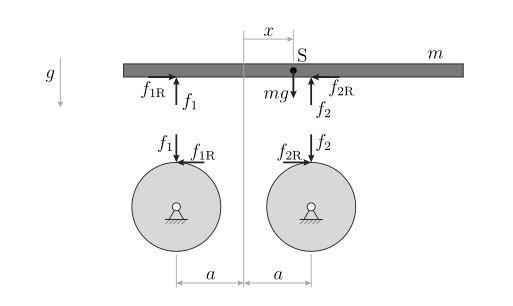
\includegraphics[width= 13cm]{tikz/03_02_2017_3a}
\end{figure}
\newline
Aufgrund der großen Winkelgeschwindigkeit gilt für die trockene Haftreibung immer $\text{sign}(\dot{x}) = 1$ und daraus kann man 
\begin{align*}
	f_{1R} &= \mu_1 f_1 \\
	f_{2R} &= \mu_2 f_2 
\end{align*}
\newpage
\noindent
b)\\ \\
Die Kräfte- und Momentenbilanz für den Balken lautet
\begin{align*}
	f_1 + f_2 - mg &= 0 \\
	-(a + x)f_1 + (a - x)f_2 &= 0
\end{align*}
Aus der ersten der beiden Gleichungen folgt
\[
	f_1 = mg - f_2
\]
Nun wird die zweite Gleichung auf $f_2$ umgeformt.
\[ 
	f_2 = \frac{(a + x)f_1}{a - x}
\]
Setzt man nun diese Gleichung in die erste ein folgt
\begin{align*}
	f_1 &= mg - \frac{(a + x)f_1}{a - x} \\
	f_1(a - x) &= mg(a - x) - (a + x)f_1 \\
	2af_1 &= mg (a - x) \\
	f_1 &= \frac{mg(a - x)}{2a}
\end{align*}
Somit folgt für die andere Normalkraft
\[
	f_2 = \frac{mg (a + x)}{2a}
\]
c)\\ \\
Impulserhaltungssatz
\[
	m\ddot{x} = \mu_1 f_1 - \mu_2 f_2
\]
d)\\ \\
Zuerst setzt man $f_1$ und $f_2$ ein. Dadurch erhält man die Differentialgleichung
\begin{align*}
	m\ddot{x} &= \mu \frac{mg(a - x)}{2a} - \mu\frac{mg (a + x)}{2a} \\
	\ddot{x} &= \mu \frac{g}{2a}(-2x) \\
	\ddot{x} + &\frac{\mu g}{a}x = 0
\end{align*}
Setzt man nun den gegebenen Ansatz in diese Gleichung ein erhält man
\begin{align*}
	\underbrace{\left(-\omega^2 + \frac{\mu g}{a}\right)}_{\overset{!}{=} 0} (A\sin(\omega t) + B\cos(\omega t)) = 0
\end{align*}
Dies führt zur Schwingungskreisfrequenz
\[
	\omega = \sqrt{\frac{\mu g}{a}}
\]
e)\\ \\
Mit den Anfangsbedingungen $x(0) = \dot{x}(0) = 0$ entsteht keine Bewegung beim Brett. \\ \\
f)\\ \\
Mit $\mu_1 \neq \mu_2$ entstehen auch bei x(0) = 0 unterschiedlich große Reibkräfte, welche zu einer resultierenden Kraft für eine Bewegung in x-Richtung führt. Es folgt eine harmonische Schwingung um einen Punkt $x \neq 0$ da mit $\mu_1 \neq \mu_2$ die Symmetrie aufgehoben wird.
	
	\subsection{31.03.2017}
	\textbf{Beispiel 1}\\ \\
a)\\ \\
i)\\ \\
Die Masse des Aufbaues lautet
\[
	m_a = (l + l_1)bh\rho
\]
Um den gesuchten Vektor zu ermitteln, müssen zuerst die Schwerpunktsvektoren der Einzelvolumina bestimmt werden. Anschließend kann dann der gtesuchte Vektor bestimmt werden und dieser lautet
\[
	\textbf{s}_a = \frac{1}{l + l_1}\begin{bmatrix}
		bl_1 \\
		\frac{l^2}{2} + ll_1 - \frac{l_1^2}{2}
	\end{bmatrix}
\]
ii)\\ \\
Sämtliche Formel die zur Berechnung benötigt werden stehen in der Formelsammlung. Durch die korrekte Anwendung dieser Formel ergeben sich für die Trägheitsmomente der seperaten Volumina
\begin{align}
	\varTheta_{\overline{y}\,\overline{y},Q1}^{(S)} &= h\rho\frac{b^3l + bl^3}{12} \\
	\varTheta_{\overline{y}\,\overline{y},Q2}^{S} &= h\rho\frac{b^3l_1 + bl_1^3}{12}
\end{align}
Mithilfe des Satz von Steiner kann nun das gesuchte Massenträgheitsmoment bestimmt werden.
\[
	\varTheta_{\overline{y}\,\overline{y},a} = \varTheta_{\overline{y}\,\overline{y},Q1} + m_{Q1}(\textbf{s}_{Q1} - \textbf{s}_a)^T(\textbf{s}_{Q1} - \textbf{s}_a) + \varTheta_{\overline{y}\,\overline{y},Q2} + m_{Q2}(\textbf{s}_{Q2} - \textbf{s}_a)^T(\textbf{s}_{Q2} - \textbf{s}_a) 
\]
mit den Massen
\[
	m_{Q1} = lbh\rho \qquad m_{Q2} = l_1bh\rho
\]
und den Vektoren
\[
	\textbf{s}_{Q1} = \begin{bmatrix}
		0 \\
		\frac{l}{2}
	\end{bmatrix}
	\qquad
	\textbf{s}_{Q2} = \begin{bmatrix}
		b \\
		l - \frac{l_1}{2}
	\end{bmatrix}
\]
b)\\ \\
Der Schwerpunktsvektor des Rades lautet
\[
	\textbf{r}_r = \begin{bmatrix}
		\alpha R \\
		0
	\end{bmatrix}
\]
und der des Aufbaues lautet
\[
	\textbf{r}_a = \begin{bmatrix}
		\alpha R + s_{ax}\cos(\beta) + s_{az}\sin(\beta) \\
		- s_{ax}\sin(\beta) + s_{az}\cos(\beta)
	\end{bmatrix}
\]
Die jeweiligen Geschwindigkeitsvektoren lauten
\begin{align*}
	\textbf{v}_r &= \begin{bmatrix}
		\dot{\alpha}R \\
		0
	\end{bmatrix} \\
	\textbf{v}_a &= \begin{bmatrix}
		\dot{\alpha}R + \dot{\beta}(-s_{ax}\sin(\beta) + s_{az}\cos(\beta)) \\
		\dot{\beta}(- s_{ax}\cos(\beta) - s_{az}\sin(\beta))
	\end{bmatrix}
\end{align*}
c)\\ \\
Die beiden gewünschten Energien lauten hier
\begin{align*}
	V = mgs_{az}\cos(\beta) \\
\end{align*}
Um die kinetische Energie zu bestimmen müssen zuerst wieder einmal Nebenrechnungen durchgeführt werden.
\begin{align*}
	\textbf{v}_r^T\textbf{v}_r &= \dot{\alpha}^2R^2 \\
	\textbf{v}_a^T\textbf{v}_a &= (\dot{\alpha}R + \dot{\beta}(-s_{ax}\sin(\beta) + s_{az}\cos(\beta)))^2 + (\dot{\beta}(-s_{ax}\cos(\beta) - s_{az}\sin(\beta)))^2 \\
	&= \dot{\alpha}^2R^2 + \dot{\beta}^2s^2_{az} + 2\dot{\alpha}R\dot{\beta}s_{az}\cos(\beta)
\end{align*}
Die kinetische Energie lautet
\[
	T = \frac{1}{2}m_a\left(\dot{\alpha}^2R^2 + \dot{\beta}^2s^2_{az} + 2\dot{\alpha}R\dot{\beta}s_{az}\cos(\beta)\right) + \frac{1}{2}m_r\dot{\alpha}^2R^2 + \frac{1}{2}\Theta_{yy,a}\dot{\beta}^2 + \frac{1}{2}\Theta_{yy,r}\dot{\alpha}^2
\]
d)\\ \\
Der Vektor für die generalisierten Kräfte kann unmittelbar aus der Angabe ermittelt werden und lautet daher
\[
	\textbf{f} = \begin{bmatrix}
		\tau_a + FR \\
		Fl\cos(\beta)
	\end{bmatrix}
\]
e)\\ \\
Für den Euler-Lagrange-Formalismus müssen erst einmal die nötigen Ableitungen durchgeführt werden. Für diese wiederum wird die Lagrange-Funktion benötigt und diese lautet hier
\begin{align*}
	L &= T - V \\
	  &= \frac{1}{2}m_a\left(\dot{\alpha}^2R^2 + \dot{\beta}^2s^2_{az} + 2\dot{\alpha}R\dot{\beta}s_{az}\cos(\beta)\right) + \frac{1}{2}m_r\dot{\alpha}^2R^2 + \frac{1}{2}\Theta_{yy,a}\dot{\beta}^2 + \frac{1}{2}\Theta_{yy,r}\dot{\alpha}^2 - mgs_{az}\cos(\beta)
\end{align*}
\newpage
\noindent
Die nötigen Ableitungen lauten
\begin{align*}
	\frac{\partial L}{\partial \alpha} &= 0 \\
	\frac{\partial L}{\partial \beta} &= -m_a\dot{\alpha}R\dot{\beta}s_{az}\sin(\beta) + mgs_{az}\sin(\beta) \\
	\frac{\partial L}{\partial \dot{\alpha}} &= m_a \dot{\alpha}R^2 + m_aR\dot{\beta}s_{az}\cos(\beta) + m_r\dot{\alpha}R^2 + \Theta_{yy,r}\dot{\alpha} \\
	\frac{\partial L}{\partial \dot{\beta}} &= m_a\dot{\beta}s^2_{az} + m_a\dot{\alpha}Rs_{az}\cos(\beta) + \Theta_{yy,a}\dot{\beta}
\end{align*}
Die notwendigen Zeitableitungen lauten
\begin{align*}
	\frac{\text{d}}{\text{d}t}\frac{\partial L}{\partial \dot{\alpha}} &= m_a\ddot{\alpha}R^2 + m_aR\ddot{\beta}s_{az}\cos(\beta) - m_aR\dot{\beta}^2s_{az}\sin(\beta) + m_r\ddot{\alpha}R^2 + \Theta_{yy,r}\ddot{\alpha} \\
	&= (\Theta_{yy,r} + (m_a + m_r)R^2)\ddot{\alpha} + \left(\cos(\beta)\ddot{\beta} - \sin(\beta)\dot{\beta}^2\right)m_aRs_{az} \\
	\frac{\text{d}}{\text{d}t}\frac{\partial L}{\partial \dot{\beta}} &= m_a\ddot{\beta}s^2_{az} + m_a\ddot{\alpha}Rs_{az}\cos(\beta) - m_a\dot{\alpha}\dot{\beta}Rs_{az}\sin(\beta) + \Theta_{yy,a}\ddot{\beta} \\
	&= (\Theta_{yy,a} + m_as^2_{az})\ddot{\beta} + \cos(\beta)\ddot{\alpha}m_aRs_{az} - m_a\dot{\alpha}R\dot{\beta}s_{az}\sin(\beta)
\end{align*}
Die Form der Euler-Lagrange-Gleichung sind in der Formelsammlung ersichtlich und diese lauten daher
\[
	\begin{bmatrix}
		 (\Theta_{yy,r} + (m_a + m_r)R^2)\ddot{\alpha} + \left(\cos(\beta)\ddot{\beta} - \sin(\beta)\dot{\beta}^2\right)m_aRs_{az} \\
		 (\Theta_{yy,a} + m_as^2_{az})\ddot{\beta} + \cos(\beta)\ddot{\alpha}m_aRs_{az} - mgs_{az}\sin(\beta)
	\end{bmatrix}
	=
	\begin{bmatrix}
		\tau_a + FR \\
		Fl\cos(\beta)
	\end{bmatrix}
\]
f)\\ \\
Mit den angegebenen Bedingungen folgt aus den Bewegungsgleichungen
\[
	\begin{bmatrix}
	\tau_a + FR \\
	Fl\cos(\beta)
	\end{bmatrix}
	=
	\begin{bmatrix}
		0 \\
		- gm_as_{az}\sin(\beta)
	\end{bmatrix}
\]
Hieraus folgt für das gesuchte Moment
\[
	\tau_a = - FR
\]
und den gesuchten Winkel
\begin{align*}
	Fl\cos(\beta) &= - gm_as_{az}\sin(\beta) \\
	-\tan(\beta) &= \frac{Fl}{s_{az}m_ag} \\
	\beta &= - \arctan\left(\frac{Fl}{s_{az}m_ag}1\right)
\end{align*}
	\newpage
\noindent
\textbf{Beispiel 2}\\ \\
a)\\ \\
Freigeschnittene Platte und Walze:
\begin{figure}[h]
	\centering
	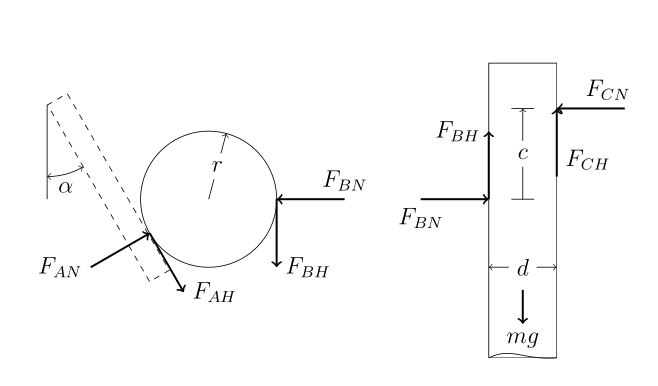
\includegraphics[width= 12.5cm]{tikz/31_03_2017_2a}
\end{figure}
\newline
b)\\ \\
Durch Aufstellen der Kräfte- und Momentenbilanz und mit der Formel für die trockene Haftreibung
\[
	f_C = \mu_Cf_N\text{sign}(\dot{x}) \qquad \text{mit sign}(\dot{x}) = 1
\]
folgt der Reibungskoeffizient
\[
	\mu_W \geq \frac{\sin(\alpha)}{1 + \cos(\alpha)}
\]
c)\\ \\
Durch Aufstellen der Kräfte- und Momentenbilanz  kann die gesuchte Höhe bestimmt werden, die die beiden Momente der Kräfte $F_{CN}$ und $F_{BN}$ ausgleicht. Die Höhe beträgt
\[
	c = \frac{d\sin(\alpha)}{2(1 + \cos(\alpha))}
\]
d)\\ \\
Da die beiden Reibungskoeffizienten nicht vom Gewicht der Platte abhängen, kann die Kraft (bis zur plastischen Verformung) theoretisch unendlich groß sein.
	\newpage
\noindent
\textbf{Beispiel 3}\\ \\
a)\\ \\
Die gesuchte Verlustwärmestromdichte wird aus der Formelsammlung entnommen lautet
\[
	\dot{q} = k(T_i - T_a)
\]
mit dem Vorfaktor (aus der Formelsammlung)
\[
	k = \frac{1}{\frac{1}{\alpha_i} + \frac{\delta_w + \delta_p}{\lambda_w} + \frac{1}{\alpha_a}}
\]
b)\\ \\
Dadurch das ein unveränderter Wärmeverlust gefordert ist folgt
\[
	\dot{q} = \dot{q}_{neu}
\]
Wegen der Dirichlet'schen Randbedingung zufolge der integrierten Wandheizung folgt
\[
	\dot{q}_{neu} = k_{neu}(T_p - T_a)
\]
und dadurch
\[
	k(T_i - T_a) = k_{neu}(T_p - T_a)
\]
mit
\[
	k_{neu} = \frac{1}{\frac{\delta_d}{\lambda_d} + \frac{\delta_w}{\lambda_w} + \frac{1}{\alpha_a}}
\]
Aus den letzten beiden Gleichungen folgt schließlich
\[
	\delta_d = \lambda_d\left(\frac{T_h - T_a}{k(T_i - T_a)} - \frac{\delta_w}{\lambda_w} - \frac{1}{\alpha_a}\right)
\]
c)\\ \\
Der Temperaturverlauf lautet
\[
	T(x) = \left\{
	\begin{array}{lll}
	T_h & \text{für} \quad 0 \leq x \leq \delta_p \\
	T_h - \dot{q}\frac{x - \delta_p}{\lambda_d} & \text{für} \quad \delta_p \leq x \leq \delta_p + \delta_d\\
	T_h - \dot{q}\left(\frac{\delta_d}{\lambda_d} + \frac{x - \delta_p - \delta_d}{\lambda_w}\right) & \text{für} \quad \delta_p + \delta_d \leq x \leq \delta_p + \delta_d + \delta_w
	\end{array}
	\right.
\]
d)\\ \\
Durch Zusammenfassen der Konturen b und w folgt aus der Summationsregel
\[
	F_{h,d} = 1 - F_{h,b+w} - F-{h,h}
\]
Da die Kontur h eine ebene Wand ist, gilt $F_{h,h} = 0$. Der andere Sichtfaktor kann mittels der Tabelle aus der Formelsammlung ermittelt werden und somit folgt
\[
	F_{h,d} = 1 - \frac{1}{2l_H}\left(l_H + \sqrt{l_b^2 + l_w^2} - \sqrt{l_b^2 + (l_w - l_h)^2}\right)	
\]
\newpage
\noindent
e)\\ \\
Da es sich bei der Kontur b ebenfalls um eine ebene Wand handelt gilt $F_{b,b} = 0$. Mit der Summationsregel und dem Reziprozitätsgesetz folgt für die restlichen Sichtfaktoren
\begin{align*}
	F_{b,h} &= \frac{l_h}{l_b}F_{b,u} \\
	F_{u,h} &= \frac{l_h}{l_1 + l_2 + l_w}F_{h,u} \\
	F_{u,b} &= \frac{l_b}{l_1 + l_2 + l_w}F_{b,u} \\
	F_{u,u} &= 1 - \frac{1}{l_1 + l_2 + l_w}(l_bF_{b,u} + l_hF_{h,u})
\end{align*}
f)\\ \\
Die gesuchte Gleichung lautet 
\[
	\varepsilon(\textbf{E} - \textbf{F}(1 - \varepsilon))^{-1}(\textbf{E} - \textbf{F})\sigma\begin{bmatrix}
	T_h^4\\ T_u^4 \\ T_b^4
	\end{bmatrix}
	+
	\begin{bmatrix}
		\dot{q}_h \\ 0 \\ 0
	\end{bmatrix}
	-
	\begin{bmatrix}
		k_2(T-h - T_a) \\ 0 \\ 0
	\end{bmatrix}
	= \textbf{\text{0}}
\]
mit
\[
	\textbf{F} = \begin{bmatrix}
		0 & F_{h,u} & F_{h,b} \\
		F_{u,h} & F_{u,u} & F_{u,b} \\
		F_{b,h} & F_{b,u} & 0  
	\end{bmatrix}
	,
	\qquad
	k_2 = \frac{1}{\frac{\delta_w}{\lambda_w} + \frac{\delta_d}{\lambda_d} + \frac{1}{\alpha_a}}
\]
Der genaue Rechenweg ist im Vorlesungsskript aus dem Jahr 2019 nachzulesen.
	
	\subsection{19.05.2017}
	\textbf{Beispiel 1}\\ \\
a)\\ \\
Die geeigneten generalisierten Koordinaten für dieses Beispiel sind
\[
	\textbf{q} = \begin{bmatrix}
		\varphi_1 & \varphi_2 & \varphi_3
	\end{bmatrix}^T
\]
Die Ortsvektoren zu den 3 Schwerpunkten lauten
\begin{align*}
	\textbf{r}_1 &= \begin{bmatrix}
	 0 \\
	 h
	\end{bmatrix}
	+
	\frac{l_1}{6}
	\begin{bmatrix}
		\cos(\varphi_1) \\
		\sin(\varphi_1)
	\end{bmatrix} \\
	\textbf{r}_2 &= \begin{bmatrix}
	 	0 \\
	 	h
	\end{bmatrix}
	+
	\frac{2l_1}{3}
	\begin{bmatrix}
		\cos(\varphi_1) \\
		\sin(\varphi_1)
	\end{bmatrix}
	+
	\frac{l_2}{2}
	\begin{bmatrix}
		\cos(\varphi_2) \\
		\sin(\varphi_2)
	\end{bmatrix} \\
	\textbf{r}_3 &= \begin{bmatrix}
	0 \\
	h
	\end{bmatrix}
	+
	\frac{l_1}{3}
	\begin{bmatrix}
		-\cos(\varphi_1) \\
		-\sin(\varphi_1)
	\end{bmatrix}
	+
	\frac{l_3}{2}
	\begin{bmatrix}
		-\cos(\varphi_3) \\
		-\sin(\varphi_3)
	\end{bmatrix}
\end{align*}
\newpage
\noindent
b) \\ \\
Die entsprechenden Geschwindigkeitsvektoren lauten
\begin{align*}
	\dot{\textbf{r}}_1 &= \frac{l_1}{6}\begin{bmatrix}
		-\sin(\varphi_1) \\
		\cos(\varphi_1)
	\end{bmatrix} \dot{\varphi_1} \\
	\dot{\textbf{r}}_2 &= \frac{2l_1}{3}\begin{bmatrix}
	-\sin(\varphi_1) \\
	\cos(\varphi_1)
	\end{bmatrix} \dot{\varphi_1}
	+ \frac{l_2}{2}\begin{bmatrix}
		-\sin(\varphi_2) \\
		\cos(\varphi_2)
	\end{bmatrix}\dot{\varphi_2} \\
	\dot{\textbf{r}}_3 &= \frac{l_1}{3}\begin{bmatrix}
		\sin(\varphi_1) \\
		-\cos(\varphi_1)
	\end{bmatrix}\dot{\varphi_1}
	+ \frac{l_3}{2}\begin{bmatrix}
		\sin(\varphi_3) \\
		-\cos(\varphi_3)
	\end{bmatrix}\dot{\varphi_3}
\end{align*}
Und deren Betragbeträge lauten
\begin{align*}
	||\dot{\textbf{r}}_1||_2^2 &= \left(\frac{l_1}{6}\right)^2 (\sin^2(\varphi_1) + \cos^2(\varphi))\dot{\varphi}^2\\ 
	&= \left(\frac{l_1}{6}\right)^2\dot{\varphi}^2 \\
	||\dot{\textbf{r}}_2||_2^2 &= \left(-\frac{2l_1}{3}\sin(\varphi_1)\dot{\varphi_1} - \frac{l_2}{2}\sin(\varphi_2)\dot{\varphi_2}\right)^2
	+
	\left(\frac{2l_1}{3}\cos(\varphi_1)\dot{\varphi_1} + \frac{l_2}{2}\cos(\varphi_2)\dot{\varphi_2}\right)^2 \\
	&= \left(\frac{2l_1}{3}\right)^2\dot{\varphi_1}^2\sin^2(\varphi_1) + \frac{2}{3}l_1l_2\sin(\varphi_1)\sin(\varphi_2)\dot{\varphi_1}\dot{\varphi_2} + \left(\frac{l_2}{2}\right)^2\dot{\varphi_2}^2\sin^2(\varphi_2) \\
	&+ \left(\frac{2l_1}{3}\right)^2\dot{\varphi_1}^2\cos^2(\varphi_1) + \frac{2}{3}l_1l_2\dot{\varphi_1}\dot{\varphi_2}\cos(\varphi_1)\cos(\varphi_2) + \left(\frac{l_2}{2}\right)^2\dot{\varphi_2}^2\cos^2(\varphi_2) \\
	&= \left(\frac{2l_1}{3}\right)^2\dot{\varphi_1}^2\left(\sin^2(\varphi) + \cos^2(\varphi_1)\right) + \left(\frac{l_2}{2}\right)^2\dot{\varphi_2}^2\left(\sin^2(\varphi_2) + \cos^2(\varphi_2)\right) \\
	&+ \frac{2}{3}l_1l_2\dot{\varphi_1}\dot{\varphi_2}\left(\cos(\varphi_1)\cos(\varphi_2) + \sin(\varphi_1)\sin(\varphi_2)\right) \\
	&=  \left(\frac{2l_1}{3}\right)^2\dot{\varphi_1}^2 + \left(\frac{l_2}{2}\right)^2\dot{\varphi_2}^2 + \frac{2}{3}l_1l_2\cos(\varphi_1 - \varphi_2)\dot{\varphi_1}\dot{\varphi_2} \\
	\text{analog dazu}: \\
	||\dot{\textbf{r}}_3||_2^2 &= \left(\frac{l_1}{3}\right)^2\dot{\varphi_1}^2 + \left(\frac{l_3}{2}\right)^2\dot{\varphi_3}^2 + \frac{1}{3}l_1l_3\cos(\varphi_1 - \varphi_3)\dot{\varphi_1}\dot{\varphi_3}
\end{align*}
	\textbf{Beispiel 2}\\ \\
a)\\ \\
Die Anzahl der Freiheitsgrade, die dieses System komplett beschreiben lautet 1, weil es hier nur eine Größe existiert die sich durch eine Bewegung des Systems ändert.\\ \\
b)\\ \\
Freigeschnittene Brücke:
\begin{figure}[h]
	\centering
	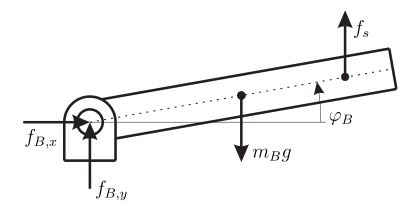
\includegraphics[width= 12.5cm]{tikz/19_05_2017_2b}
\end{figure}
\newline
Das gesuchte Kräftegleichgewicht lautet
\begin{align*}
	\textbf{e}_x &: f_{B,x} = 0 \\
	\textbf{e}_y &: f_{B,y} - m_Bg + f_s = 0
\end{align*}
und das Momentengleichwicht lautet
\[
	\textbf{e}_z : -m_Bgl_B\cos(\varphi_B) + f_sl_s\cos(\varphi_B) = 0
\]
Um die Seilkraft zu bestimmen muss nur das Momentengleichwicht in Betracht gezogen werden.
\begin{align*}
	-m_Bgl_B\cos(\varphi_B) &+ f_sl_s\cos(\varphi_B) = 0 \\ 
	 f_sl_s\cos(\varphi_B) &= m_Bgl_B\cos(\varphi_B) \\
	 f_s &=  m_Bg\frac{l_B}{l_s}
\end{align*}
\newpage
\noindent
c) \\ \\
Freigeschnittener Träger:
\begin{figure}[h]
	\centering
	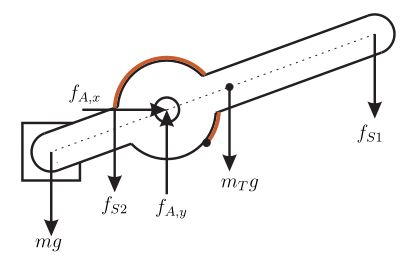
\includegraphics[width= 10 cm]{tikz/19_05_2017_2c}
\end{figure}
\newline
Hier lautet das Kräftegleichgewicht
\begin{align*}
	\textbf{e}_x &: f_{A,x} = 0 \\
	\textbf{e}_y &: -mg - f_{S2} + f_{A,y} - m_Tg - f_{S1} = 0
\end{align*}
und das Momentengleichgewicht
\[
	\textbf{e}_z: mgl_m\cos(\varphi_B) + f_{S2}R - m_Tgl_T\cos(\varphi_B) - f_{S1}l_s\cos(\varphi_B) = 0
\]
Um wieder die fehlende Seilkraft zu bestimmen muss wieder nur das Momentengleichwicht betrachtet werden. Daher lautet diese
\begin{align*}
	mgl_m\cos(\varphi_B) + f_{S2}R - m_Tgl_T\cos(\varphi_B) - f_{S1}l_s\cos(\varphi_B) = 0 \\
	mgl_m\cos(\varphi_B) + f_{S2}R - m_Tgl_T\cos(\varphi_B) - m_Bgl_B\cos(\varphi_B) = 0 \\
	f_{S2} = \frac{m_Bgl_B + m_Tgl_T - mgl_m}{R}\cos(\varphi_B)
\end{align*}
d)\\ \\
Um die gesuchte Masse zu bestimmen, muss man beachten das die Kraft $f$ gleich der Kraft $f_{S2}$ sein, d.h. man muss die beiden gleichsetzen. Daraus folgt
\begin{align*}
	\frac{m_Bgl_B + m_Tgl_T - mgl_m}{R}\cos(\varphi_B) = 0 \\
	m_Bgl_B + m_Tgl_T - mgl_m = 0 \\
	m = \frac{m_Bl_B + m_Tl_T}{l_m}
\end{align*}
\newpage
\noindent
e)\\ \\
Die Formel zu Berechnung des Massenträgheitsmoment kann der Formelsammlung entnommen werden.
\begin{align*}
	\varTheta_B &= \int_{\mathcal{V}}r^2\text{d}m = \rho \int_{\mathcal{V}}r^2\text{d}V \\
	&= \rho b \int_{0}^{l}\int_{-\frac{d}{2}}^{\frac{d}{2}}(y^2 + z^2)\text{d}z\text{d}y \\
	&= \rho b \int_{0}^{l}\left(y^2z + \frac{z^3}{3}\right)\biggl|^{\frac{d}{2}}_{-\frac{d}{2}}\text{d}y \\
	&= \rho b \int_{0}^{l}\left(y^2\frac{d}{2} + \frac{d^3}{16} + y^2\frac{d}{2} + \frac{d^3}{24}\right)\text{d}y \\
	&= \rho b \int_{0}^{l}\left(y^2d + \frac{d^3}{12}\right)\text{d}y \\
	&= \rho b \left(\frac{y^3}{3}d + \frac{d^3}{12}y\right)\biggl|^{l}_0 \\
	&= \rho b \left(\frac{l^3}{3}d + \frac{d^3}{12}l\right)
\end{align*}
Mit $m_B = \rho lbd$ folgt
\[
	\varTheta_B = m_B\left(\frac{l^2}{3} + \frac{d^2}{12}\right)
\]
f)\\ \\
Wenn nun das Seil 1 reißt wird die Brücke fallen. Da sich hier dann um eine Drehbewegung handelt besitzt die kinetische Energie der Brücke nur einen rotatorischen Anteil und lautet somit
\[
	T = \frac{1}{2}\varTheta_B\dot{\varphi}^2_B
\]
Die potentielle Energie zum Zeitpunkt $t = 0$ lautet
\[
	V = m_B g l_B \sin(\varphi_0)
\]
Da die Energieerhaltung erfüllt sein muss folgt für die gesuchte Winkelgeschwindigkeit
\begin{align*}
	T &+ V = 0 \\
	\frac{1}{2}\varTheta_B\dot{\varphi}_B^2 &+ m_B g l_B \sin(\varphi_0) = 0 \\
	\dot{\varphi}_B &= - \sqrt{\frac{2m_Bgl_B}{\varTheta_B}\sin(\varphi_0)} 
\end{align*}
	\newpage
\noindent
\textbf{Beispiel 3}\\ \\
a)\\ \\
Die richtige Formel für die Konvektion kann aus der Formelsammlung entnommen werden. Daher lautet die gesuchte Wärmestromdichte
\[
	\dot{q}_{aw}(x,t) = \alpha_{aw}\left(T_a(x,t) - T_w(x,t)\right)
\]
b)\\ \\
Die gesuchte Wärmestromdichten können mittels des Wärmeleitgesetzes bestimmt werden und lauten somit
\begin{align*}
	\dot{q}_a &= -\lambda\frac{\partial}{\partial x}T_a(x,t) \\
	\dot{q}_w &= -\lambda\frac{\partial}{\partial x}T_w(x,t)
\end{align*}
c)\\ \\
Mithilfe des Hinweises aus der Angabe und der Wärmeleitgleichung für kartesische Koordinaten lautet die gesuchte Differentialgleichung
\[
	\rho_a c_a \frac{\partial}{\partial t}T_a(x,t) = \lambda\frac{\partial^2}{\partial x^2}T_a(x,t) + \frac{\alpha_a}{d_a}\dot{q}_s - \frac{\alpha_{aw}}{d_w}\left(T_a(x,t) - T_w(x,t)\right)
\]
Der zweite und der dritte Term auf der rechten Seite der Gleichung sind der zufließende und abfließende Wärmestrom aus dem Kontrollvolumen. \\ \\
d)\\ \\
Analog zu Punkt c) lautet die Differentialgleichung hier
\begin{align*}
	\underbrace{\rho_wc_w\frac{\partial}{\partial t}T_w(x,t) = \lambda\frac{\partial^2}{\partial x^2}T_w(x,t) - \rho_wc_wv_w\frac{\partial}{\partial x}T_w(x,t)}_{\text{Wärmeleitgleichung}} + \frac{\alpha_{aw}}{d_w}\left(T_a(x,t) - T_w(x,t)\right) \\
	\rho_w c_w \left(\frac{\partial}{\partial t}T_w(x,t) + v_w\frac{\partial}{\partial x}T_w(x,t)\right) = \lambda\frac{\partial^2}{\partial x^2}T_w(x,t) + \frac{\alpha_{aw}}{d_w}\left(T_a(x,t) - T_w(x,t)\right)
\end{align*}
e)\\ \\
Für das gesamte System werden hier 4 Randbedingungen benötigt. Nämlich 2 pro Differentialgleichung.\\ \\
f)\\ \\
Die Randbedingungen dieses Systems lauten 
\begin{align*}
	\dot{q}_a(0,t) &= \dot{q}_a(L,t) = 0 \\
	T_w(0,t) &= T_w^{in}(t) \\
	\dot{q}_w(L,t) &= 0
\end{align*}
	
	\subsection{14.07.2017}
	\textbf{Beispiel 1}\\ \\
a)\\ \\
Um den gesuchten Abstand zu ermitteln, muss man die Formel
\[
	\textbf{r}_S = \frac{\sum_{j=1}^{N}\textbf{r}_{Sj}m_j}{\sum_{j=1}^{N}m_j}
\]
betrachten. Unter Beachtung dieser Form folgt nun schließlich für den gesuchten Abstand
\begin{align*}
	l_{AM} &= \frac{m_Al_A - m_Ml_M}{m_{AM}} 
\end{align*}
mit $m_{AM} = m_A + m_M$. Dies hat nur eine Ähnlichkeit mit der obigen Formel, da anstatt von Abstandsvektoren nur die tatsächlichen Abstände verwendet wurden. Das dazugehörige Massenträgheitsmoment kann schließlich mit dem Satz von Steiner ermittelt werden und lautet somit
\[
	\varTheta_{AM,zz} = \varTheta_{A,zz} + m_A(l_A - l_{AM})^2 + \varTheta_{M,zz} + m_M(l_{AM} + l_M)^2
\]
b)\\ \\
Die geeigneten generalisierten Koordinaten lauten hier
\[
	\textbf{q} = \begin{bmatrix}
		x \\
		\varphi_A
	\end{bmatrix}
\]
und somit lautet der Ortsvektor der Ersatzmasse
\[
	\textbf{r}_{AM} = l_{AM}\begin{bmatrix}
		-\sin(\varphi_A) \\
		\cos(\varphi_A)
	\end{bmatrix}
\]
und der Ortsvektor des Schlittens
\[
	\textbf{r}_S = x\begin{bmatrix}
		-\sin(\varphi_A) \\
		\cos(\varphi_A)
	\end{bmatrix}
\]
c)\\ \\
Nun müssen man für die Geschwindigkeitsvektoren die Ortsvektoren nach den generalisierten Koordinaten ableiten. Damit erhalten wir
\begin{align*}
	\dot{\textbf{r}}_{AM} &= l_{AM}\begin{bmatrix}
		-\cos(\varphi_A) \\
		-\sin(\varphi_A)
	\end{bmatrix}\dot{\varphi}_A
	\\ \\
	\dot{\textbf{r}}_S &= x\begin{bmatrix}
		-\cos(\varphi_A) \\
		-\sin(\varphi_A)
	\end{bmatrix}\dot{\varphi}_A
	+\dot{x}
	\begin{bmatrix}
		-\sin(\varphi_A) \\
		\cos(\varphi_A)
	\end{bmatrix}
\end{align*}
\newpage
\noindent
Deren Betragsquadrate lauten
\begin{align*}
	||\dot{\textbf{r}}_{AM}||^2_2 &= l^2_{AM}\left(\sin^2(\varphi_A) + \cos^2(\varphi_A)\right)\dot{\varphi}_A^2 \\
				 				  &= l^2_{AM}\dot{\varphi}_A^2 \\ \\
	||\dot{\textbf{r}}_{S}||^2_2 &=	x^2\left(\sin^2(\varphi_A) + \cos^2(\varphi_A)\right)\dot{\varphi}_A^2 + \dot{x}^2\left(\sin^2(\varphi_A) + \cos^2(\varphi_A)\right)	\\
	&= x^2\dot{\varphi}_A^2 + \dot{x}^2
\end{align*}
d)\\ \\
Die kinetische Energie des gesamten Systems lautet
\begin{align*}
	T &= \frac{1}{2}m_{AM}||\dot{\textbf{r}}_{AM}||^2_2 + \frac{1}{2}m_S||\dot{\textbf{r}}_{S}||^2_2 + \frac{1}{2}(\varTheta_{AM,zz} + \varTheta_{S,zz})\dot{\varphi}_A^2 \\
	&= \frac{1}{2}m_{AM}l^2_{AM}\dot{\varphi}_A^2 + \frac{1}{2}m_S\left(x^2\dot{\varphi}_A^2 + \dot{x}^2\right) + \frac{1}{2}(\varTheta_{AM,zz} + \varTheta_{S,zz})\dot{\varphi}_A^2 \\ \\
	V &= 0
\end{align*}
e)\\ \\
Die Lagrange-Funktion lautet in allgemeiner Form
\[
	L = T - V
\]
und die Euler-Lagrange-Gleichungen
\[
	\frac{\text{d}}{\text{d}t}\frac{\partial L}{\partial \dot{q}_i} - \frac{\partial L}{\partial q_i} = f_{d,i} + f_{q,i}, \qquad i\in\{1,2\}
\]
f) \\ \\
Bevor nun die einzelnen bestimmt werden können, muss die Lagrange-Funktion konkret ausgewertet. Diese lautet daher
\[
	L = \frac{1}{2}m_{AM}l^2_{AM}\dot{\varphi}_A^2 + \frac{1}{2}m_S\left(x^2\dot{\varphi}_A^2 + \dot{x}^2\right) + \frac{1}{2}(\varTheta_{AM,zz} + \varTheta_{S,zz})\dot{\varphi}_A^2
\]
\newpage
\noindent
Die Ableitungen lautet
\begin{align*}
	\frac{\partial L}{\partial \dot{x}} &= m_S\dot{x} \\
	\frac{\partial L}{\partial \dot{\varphi}_A} &= m_{AM}l^2_{AM}\dot{\varphi}_A + m_Sl^2_S\dot{\varphi}_A + (\varTheta_{AM,zz} + \varTheta_{S,zz})\dot{\varphi}_A \\
	\frac{\text{d}}{\text{d}t}\frac{\partial L}{\partial \dot{x}} &= m_S\ddot{x} \\
	\frac{\text{d}}{\text{d}t}\frac{\partial L}{\partial \dot{\varphi}_A} &= m_{AM}l^2_{AM}\ddot{\varphi_A} + m_Sx^2\ddot{\varphi_A} + 2m_Sx\dot{\varphi}_A\dot{x} + (\varTheta_{AM,zz} + \varTheta_{S,zz})\ddot{\varphi_A} \\
	\frac{\partial L}{\partial x} &= m_Sx\dot{\varphi}_A^2 \\
	\frac{\partial L}{\partial \varphi_A} &= 0
\end{align*}
g)\\ \\
Der Vektor für die generalisierten dissipativen Kräfte lautet
\[
	\textbf{f}_d = \begin{bmatrix}
		-d_s\dot{x} \\
		-d_A\dot{\varphi}_A
	\end{bmatrix}
\]
h)\\ \\
Die Formel zur Bestimmung der generalisierten Kräfte kann der Formelsammlung entnehmen. Der benötigte Ortsvektor ist der des Schlittens. Die benötigte Ableitung für die generalisierte Kraft lautet 
\[
	\frac{\partial \textbf{r}_S}{\partial x} = \begin{bmatrix}
		-\sin(\varphi_A) \\
		\cos(\varphi_A)
	\end{bmatrix}
\]
Der Vektor der externen Kraft lautet
\[
	\textbf{f}_S = F_S\begin{bmatrix}
		\sin(\varphi_A) \\
		-\cos(\varphi_A)
	\end{bmatrix}
\]
Der Vektor der Momente bezogen auf die generalisierten Koordinaten lautet
\[
	\textbf{m}_A = \begin{bmatrix}
		0 \\
		M_A
	\end{bmatrix}
\]
Somit lautet der Vektor der generalisierten Kräfte
\[
	\textbf{f}^T_q = \textbf{f}_S^T	\frac{\partial \textbf{r}_S}{\partial x} + \textbf{m}^T_A = \begin{bmatrix}
		-F_S & M_A
	\end{bmatrix}^T
\]
\newpage
\noindent
i)\\ \\
Die Euler-Lagrange-Gleichungen lauten
\begin{align*}
	m_S\ddot{x} - m_Sx\dot{\varphi}_A^2 &= -d_S\dot{x} - F_S \\
	m_{AM}l^2_{AM}\ddot{\varphi_A} + m_Sx^2\ddot{\varphi_A} + 2m_Sx\dot{\varphi}_A\dot{x} &+ (\varTheta_{AM,zz} + \varTheta_{S,zz})\ddot{\varphi_A} = -d_A\dot{\varphi}_A + M_A
\end{align*}
Vereinfacht man diese Gleichungen erhält man die Bewegungsgleichungen und diese lauten
\begin{align*}
	\ddot{x} &= \frac{m_Sx\dot{\varphi}^2_A - d_S\dot{x} - F_S}{m_S} \\
	\ddot{\varphi}_A &= \frac{-2m_Sx\dot{\varphi}_A\dot{x} - d_A\dot{\varphi}_A + M_A}{m_{AM}l^2_{AM} + m_Sx^2 + (\varTheta_{AM,zz} + \varTheta_{S,zz})}
\end{align*}
j)\\ \\
Aus der ersten Bewegungsgleichung folgt im stationären Fall
\begin{align*}
		0 &= \frac{m_Sx_0\omega^2_A - F_S}{m_S} \\
		x_0 &= \frac{F_S}{m_S\omega_A^2}
\end{align*}
und aus der zweiten
\begin{align*}
	0 &= \frac{ - d_A\omega_A + M_{A,0}}{m_{AM}l^2_{AM} + m_Sx^2 + (\varTheta_{AM,zz} + \varTheta_{S,zz})} \\
	M_{A,0} &= d_A\omega_A^2	
\end{align*}
	\newpage
\noindent
\textbf{Beispiel 2}\\ \\
a)\\ \\
Freigeschnittene Objekte:
\begin{figure}[h]
	\centering
	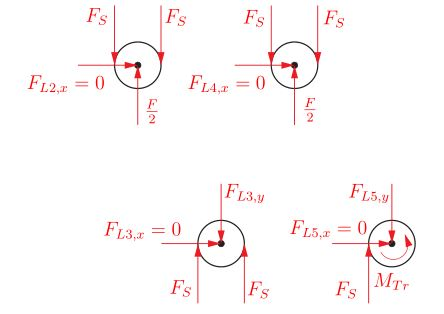
\includegraphics[width= 10cm]{tikz/17_07_2017_2a}
\end{figure}
\newline
Die benötigten Gleichgewichtsgleichungen lauten hier für die erste Umlenkrolle
\begin{align*}
	\textbf{e}_x &: F_{L2,x} = 0 \\
	\textbf{e}_y &: -2F_S + \frac{F}{2} = 0 
\end{align*}
für die zweite Umlenktrommel
\begin{align*}
	\textbf{e}_x &: F_{L3,x} = 0 \\
	\textbf{e}_y &: 2F_S - F_{L3,y} = 0 \\
\end{align*}
für die dritte Umlenkrolle
\begin{align*}
	\textbf{e}_x &: F_{L4,x} = 0\\
	\textbf{e}_y &: -2F_S + \frac{F}{2} = 0 \\
\end{align*}
und für die Trommel
\begin{align*}
	\textbf{e}_x &: F_{L5,x} = 0\\
	\textbf{e}_y &: F_S - F_{L5,y} = 0\\
	\textbf{e}_z &: M_{TR} - F_S\frac{d}{2}
\end{align*}
\newpage
\noindent
b)\\ \\
Um die benötigten Lagerkräfte zu bestimmen muss man nur die Gleichgewichtsgleichungen beachten und entsprechend umformen. Für die Seilkraft folgt aus zweiten Gleichung der ersten Rolle
\[
	F_S = \frac{F}{4}
\]
Daher lauten die Kräfte für das Lager 1 (durch freischneiden von Lager 1)
\begin{align*}
	F_{L1,x} &= 0 \\
	F_{L2,y} &= F_S = \frac{F}{4}
\end{align*}
für das Lager 3
\begin{align*}
	F_{L3,x} &= 0 \\
	F_{L3,y} &= 2F_S = \frac{F}{2}
\end{align*}
und für das Lager 5
\begin{align*}
	F_{L5,x} &= 0 \\ 
	F_{L5,y} &= F_S = \frac{F}{4}
\end{align*}
c)\\ \\
Das Trommelmoment lautet
\[
	M_{TR} = \frac{Fd}{8}
\]
Mit dem Übersetzungsverhältnis aus der Angabe folgt schließlich für das Haltemoment
\[
	M_M = \frac{Fd}{8i}
\]
	\textbf{Beispiel 3}\\ \\
a)\\ \\
Die Leistungsbilanz für das elektronische Bauteil lautet
\[
	-\dot{q}_s + g_0h - \dot{q}_b = 0
\]
und daraus folgt
\[
	\dot{q}_s = g_0h - \dot{q}_b
\]
b) \\ \\
Mit der Formel
\[
	\dot{q} = \alpha (T - T_\infty)
\]
folgt für die Oberflächentemperatur
\[
	T_s = T_\infty + \frac{\dot{q}_s}{\alpha}
\]
\newpage
\noindent
c)\\ \\
Um die Differentialgleichung bestimmen zu können muss man die Wärmeleitgleichung für die kartesischen Koordinaten hernehmen. Da sich die Wärme nur in z-Richtung ausbreitet muss auch nur dieser Term der Formel verwendet werden.
\[
	\lambda\frac{d^2T}{dz^2} + g_0 = 0
\]
Mit den Randbedingungen
\begin{align*}
	\frac{dT}{dz}(0) &= \frac{\dot{q}_b}{\lambda} \\
	T(h) &= T_s
\end{align*}
d) \\ \\
Für den Temperaturverlauf im Bauteil muss jetzt die Differentialgleichung gelöst werden.
\begin{align*}
		\lambda\frac{d^2T}{dz^2} + g_0 = 0 \\
		\frac{d^2T}{dz^2} = -\frac{g_0}{\lambda} \\
		\frac{dT}{dz} = -\frac{g_0}{\lambda}z + C_1 \\
		T(z) = -\frac{g_0}{\lambda}\frac{z^2}{2} + C_1z + C_2
\end{align*}
Durch Einsetzen der Randbedingungen folgt für die Konstanten
\begin{align*}
	\frac{dT}{dz} &= 0 + C_1 = \frac{\dot{q}_b}{\lambda} \\
	C_1 &= \frac{\dot{q}_b}{\lambda} 
\end{align*}
und
\begin{align*}
	T_s &= -\frac{g_0}{\lambda}\frac{h^2}{2} + \frac{\dot{q}_b}{\lambda}h + C_2 \\
	C_2 &= T_s + \frac{g_0}{\lambda}\frac{h^2}{2} - \frac{\dot{q}_b}{\lambda}h
\end{align*}
Jetzt noch die Konstanten einsetzen und man erhält schließlich
\begin{align*}
	T(z) &= -\frac{g_0}{\lambda}\frac{z^2}{2} + \frac{\dot{q}_b}{\lambda}z + T_s + \frac{g_0}{\lambda}\frac{h^2}{2} - \frac{\dot{q}_b}{\lambda}h \\
	&= T_s \frac{1}{2}\frac{\dot{q}_b}{\lambda}(h^2 - z^2) + \frac{\dot{q}_b}{\lambda}(z - b)
\end{align*}
\newpage
\noindent
e) \\ \\
Die maximale Position lautet
\[
	z_{max} = \frac{\dot{q}_b}{g_0}
\]
Für die maximale Temperatur existier leider keine Lösung zum vergleichen. \\ \\
	\textbf{Beispiel 4}\\ \\
a) \\ \\
Da sich bei B1 um eine konvexe Fläche handelt lautet der entsprechende Sichtfaktor
\[
	F_{11} = 0
\]
Da B2 die Sicht von B1 auf B3 blockiert gilt
\[
	F_{13} = 0
\]
Der Sichtfaktor zwischen B1 und B2 wird mit der Cross-String-Methode bestimmt.
\begin{figure}[h]
	\centering
	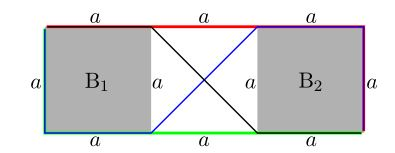
\includegraphics[width= 10cm]{tikz/17_07_2017_4a}
\end{figure}
Dieser lautet nun
\[
	F_{12} = \frac{(2a + \sqrt{2}a) + (4a + \sqrt{2}a) - 4a - 4a}{8a} = \frac{2\sqrt{2}a - 2a}{8a} = \frac{\sqrt{2} - 1}{4}
\]
Aufgrund der Geometrie gilt
\[
		F_{32} = F_{12} = \frac{\sqrt{2} - 1}{4}
\]
b) \\ \\
Mit der Summationsregel folgt
\[
	F_{14} = 1 - F_{12} = \frac{5 - \sqrt{2}}{4}
\]
Außerdem gilt durch diese Regel noch
\[
	F_{24} = 1 - F_{21} - F_{22} - F_{23}
\]
\newpage
\noindent
Da es sich bei B2 wieder um eine konvexe Fläche handelt muss wieder
\[
	F_{22} = 0
\]
gelten. Außerdem kann man aus dem Reziprozitätsgesetz
\begin{align*}
	F_{21} &= F_{12}  \\
	F_{23} &= F_{32} = F_{12}
\end{align*}
schließen. Dadurch gilt für den gesuchten Faktor
\[
	F_{24} = 1 - 2F_{12} = \frac{6 - 2\sqrt{2}}{4}
\]
Wegen der Geometrie des Problems gilt
\[
	F_{34} = F_{14} = \frac{5 - \sqrt{2}}{4}
\]
c)\\ \\
Mit dem Reziprozitätsgesetz und der Summationsregel für die benötigten Sichtfaktoren
\begin{align*}
	F_{41} &= \frac{A_1}{A_4}F_{14} = \frac{1}{6}\frac{5 - \sqrt{2}}{4} \\
	F_{42} &= \frac{A_2}{A_4}F_{24} = \frac{1}{6}\frac{6 - \sqrt{2}}{4} \\
	F_{43} &= F_{41} = \frac{1}{6}\frac{5 - \sqrt{2}}{4} \\
	F_{44} &= 1 - 2F_{41} - F_{42} = \frac{1}{6}(2 + \sqrt{2})
\end{align*}
d)\\ \\
B1 und B3 erwärmen sich schneller als B2, da die Sichtfaktoren folgendes Verhalten ausweisen.
\[
	F_{41} = F_{43} > F_{42}
\]
	
	\newpage
	\subsection{29.09.2017}
	\textbf{Beispiel 1}\\ \\
a)\\ \\
Freigeschnittene Massen:
\begin{figure}[h]
 	\centering
 	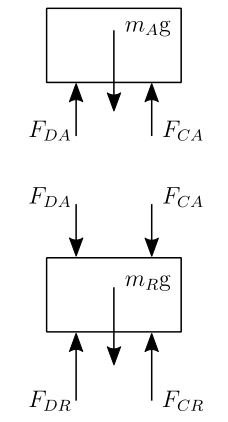
\includegraphics[width= 3cm]{tikz/29_09_2017_1a}
\end{figure}
\newline
Die Berechnungsvorschriften lauten
\begin{align*}
	F_{CA} = c_a(x_R - x_A) & F_{DA} = d_A(v_{RA})(\dot{x}_R - \dot{x}_A) \\
	F_{CR} = c_R(x_U - x_R) & F_{DR} = d_R(\dot{x}_U - \dot{x}_R)
\end{align*}
b)\\ \\
Die Bewegungsgleichungen der Massen kann mithilfe der Implulserhaltung aufgestellt werden und lauten für den Aufbau
\[
	m_A\ddot{x}_A = F_{CA} + F_{DA} - m_Ag
\]
und für das Rad
\[
	m_R\ddot{x}_R = F_{CR} + F_{DR} - F_{CA} - F_{DA} - m_Rg
\]
c)\\ \\
Im stationären Fall lauten die beiden Bewegungsgleichungen
\begin{align*}
	0 &= F_{CA} - m_Ag \\
	0 &= F_{CR} - F_{CA} - m_Rg
\end{align*}
Aus der ersten Gleichung folgt
\[
	F_{CA} = m_Ag
\]
\newpage
\noindent
Nun setzt man dies in die zweite Bewegungsgleichung ein. Das führt dann auf
\begin{align*}
	0 &= F_{CR} - m_Ag - m_Rg \\
	0 &= -c_Rx_R - m_Ag - m_Rg \\
	x_R &= -\frac{(m_A + m_R)g}{c_R}
\end{align*}
Daraus folgt für die andere Auslenkung
\begin{align*}
	F_{CA} = m_Ag &= c_a(x_R - x_A) \\
	m_Ag &= -c_A\left(\frac{(m_A + m_R)g}{c_R} + x_A\right) \\
	-\frac{m_Ag}{c_a} &= \frac{(m_A + m_R)g}{c_R} + x_A \\
	x_A &= -\frac{(m_A + m_R)g}{c_R} - \frac{m_Ag}{c_a} 
\end{align*}
d)\\ \\
Freigeschnittene Radaufhängung:
\begin{figure}[h]
	\centering
	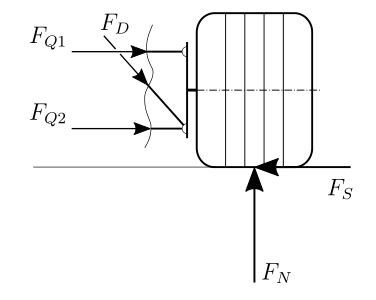
\includegraphics[width= 5cm]{tikz/29_09_2017_1d}
\end{figure}
\newline
e)\\ \\
Der Drehpunkt für die Momentengleichung ist der Schnittpunkt der Stäbe Q2 und D. Die Gleichgewichtsbedingungen für die Radaufhängung lautet daher
\begin{align*}
	\textbf{e}_x &: F_{Q1} + F_{Q2} - F_S + F_D\cos(\alpha) = 0\\
	\textbf{e}_y &: -F_D\sin(\alpha) + F_N\\
	\textbf{e}_z &: -F_{Q1}b - F_Sa + F_Nd
\end{align*}
\newpage
\noindent
Aus diesen Gleichungen können nun die gesuchten Stabkräfte bestimmt werden.
\begin{align*}
	F_D &= \frac{F_N}{\sin(\alpha)} \\
	F_{Q1} &= \frac{F_Nd - F_Sa}{b} = \frac{\frac{F_N}{\sin(\alpha)}d - F_Sa}{b} \\
	0 &= \frac{\frac{F_N}{\sin(\alpha)}d - F_Sa}{b} + F_{Q2} - F_S + \frac{F_N}{\sin(\alpha)}\cos(\alpha) \\
	F_{Q2} &= F_S\left(1 + \frac{a}{b}\right) - F_N\left(\cot(\alpha) + \frac{d}{b}\right)
\end{align*}
	\textbf{Beispiel 2}\\ \\
a)\\ \\
Dieses System wird durch einen Freiheitsgrad komplett beschrieben, z.B der Kurbelwinkel $\alpha$. \\ \\
b)\\ \\
Als geeigneter Freiheitsgrad wurde der Winkel $\alpha$ gewählt. Es gilt die Zwangsbeziehung
\[
	R_1\sin(\alpha) = R_2\sin(\beta)
\]
Dadurch lautet der Winkel $\beta$
\[
	\beta = \arcsin\left(\frac{R_1}{R_2}\sin(\alpha)\right)
\]
c)\\ \\
Die Ortsvektoren zu den Körperschwerpunkten lauten für die Kurbelwelle 
\[
	\textbf{r}_{S1} = \begin{bmatrix}
		e\cos(\alpha) \\
		e\sin(\alpha) \\ 
		0
	\end{bmatrix}
\]
die Pleuelstange
\[
	\textbf{r}_{S2} = \begin{bmatrix}
		R_1\cos(\alpha) + \frac{R_2}{2}\cos(\beta(\alpha)) \\
		\frac{R_2}{2}\sin(\beta(\alpha))
	\end{bmatrix}
\]
und der für den Kolben
\[
	\textbf{r}_K = \begin{bmatrix}
		R_1\cos(\alpha) + R_2\cos(\beta(\alpha)) \\
		0 \\
		0		
	\end{bmatrix}
\]
\newpage
\noindent
Die Geschwindigkeiten lauten für die Kurbelwelle
\[
	\textbf{v}_{S1} = \begin{bmatrix}
		-e\sin(\alpha)\dot{\alpha }\\
		e\cos(\alpha)\dot{\alpha} \\ 
		0
	\end{bmatrix}
	\qquad
	\omega_{S1} = \dot{\alpha}
\]
die Pleuelstange
\[
	\textbf{v}_{S2} = \begin{bmatrix}
		-R_1\sin(\alpha)\dot{\alpha} - \frac{R_2}{2}\sin(\beta)\frac{d\beta}{d\alpha}\dot{\alpha} \\
		\frac{R_2}{2}\cos(\beta)\frac{d\beta}{d\alpha}\dot{\alpha} \\
		0
	\end{bmatrix}
	\qquad
	\omega_{S2} = \frac{d\beta}{d\alpha}\dot{\alpha} 
\]
und für den Kolben
\[
	\textbf{v}_K = \begin{bmatrix}
		-R_1\sin(\alpha)\dot{\alpha} - R_2\sin(\beta)\frac{d\beta}{d\alpha}\dot{\alpha} \\
		0 \\
		0
	\end{bmatrix}
	\qquad
	\omega_K = 0
\]
e)\\ \\
Die kinetischen Teilenergien lauten hier
\[
	T_{rot} = \frac{1}{2}\left(\varTheta_1\dot{\alpha}^2 + \varTheta_2\left(\frac{d\beta}{d\alpha}\dot{\alpha}\right)^2\right)
\]
und 
\[
	T_{trans} = \frac{1}{2}(m_1\textbf{v}_{S1}^T\textbf{v}_{S1} + m_2\textbf{v}_{S2}^T\textbf{v}_{S2} + m_K\textbf{v}_K^T\textbf{v}_K)
\]
Daher ergibt sich für die gesamte kinetische Energie
\[
	T = T_{rot} + T_{trans}
\]
f)\\ \\
Der Ortsvektor zum Angriffspunkt der externen Kraft lautet
\[
	\textbf{r}_{F_p} = \begin{bmatrix}
	R_1\cos(\alpha) + R_2\cos(\beta(\alpha)) \\
	0 \\
	0		
	\end{bmatrix}
\]
Der Vektor der externen Kraft lautet
\[
	\textbf{f}_{F_p} = \begin{bmatrix}
		-F_p \\
		0 \\
		0
	\end{bmatrix}
\]
Die notwendige Ableitung lautet
\[
	\frac{\partial\textbf{r}_{F_p} }{\partial \alpha} = \begin{bmatrix}
	-R_1\sin(\alpha)\dot{\alpha} - R_2\sin(\beta)\frac{d\beta}{d\alpha} \\
	0 \\
	0
	\end{bmatrix}
\]
Mit der Berechnungsvorschrift für den gesuchten Vektor aus der Formelsammlung, ergibt sich für diesen
\[
	Q = F_p\left(R_1\sin(\alpha) + R_2\sin(\beta)\frac{d\beta}{d\alpha}\right) 
\]
	\newpage
\noindent
\textbf{Beispiel 3}\\ \\
a)\\ \\
Die Formel für den konvektiven Wärmeübergang wird der Formelsammlung entnommen und somit lauten die gesuchten Wärmestromdichten
\begin{align*}
	\dot{q}_{BG} &= \alpha(T_B - T_G(t)) \\ 
	\dot{q}_{MG} &= \alpha(T_M - T_G(t)) \\
	\dot{q}_{DG} &= \alpha(T_D - T_G(t))
\end{align*}
Die SI-Einheit von $\alpha$ lautet
\[
	[\alpha] = \frac{W}{m^2K}
\]
b)\\ \\
Die Sichtfaktormatrix muss die Form
\[
	\textbf{F} = \begin{bmatrix}
		F_{B-B} & F_{B-M} & F_{B-D} \\
		F_{M-B} & F_{M-M} & F_{M-D} \\
		F_{D-B} & F_{D-M} & F_{D-D}
	\end{bmatrix}
\]
besitzen. Die einzelnen Sichtfaktor werden mit der Summationsregel und dem Reziprozitätsgesetz bestimmt. Außerdem muss man auch noch beachten, ob es sich bei manchen Flächen um konvexe Flächen handelt, da sich dann die entsprechenden Sichtfaktoren einfach aufstellen lassen. Unter Beachtung all dieser Bedingungen lauten hier sämtliche Sichtfaktoren
\begin{align*}
	F_{B-B} &= F_{D-D} = 0 & F_{M-D} &= \frac{A_D}{A_M}(1 - F) \\
	F_{B-D} &= F_{D-B} = F & F_{M-B} &= \frac{A_B}{A_M}(1 - F)\\
	F_{B_M} &= F_{M-B} = 1 - F & F_{M-M} &= 1 - 2\frac{A_B}{A_M}(1 - F)
\end{align*}
c)\\ \\
Unter Beachtung der Formel für die Nettowärmestromdichte aus der Formelsammlung erhält man für die gesuchten Größen
\begin{align*}
	 \dot{\textbf{q}}_r = \begin{bmatrix}
		\dot{q}_{r,B} \\
		\dot{q}_{r,M} \\
		\dot{q}_{r,D}
	\end{bmatrix}
	, \quad
	\textbf{T}^4 = \begin{bmatrix}
		T_B^4 \\
		T_M^4 \\
		T_D^4
	\end{bmatrix}
	, \quad
	\varepsilon = \begin{bmatrix}
		\varepsilon_B \\
		\varepsilon_M \\
		\varepsilon_D
	\end{bmatrix}
	\\ \\
	\textbf{P} = \text{diag}{\varepsilon}(\textbf{E} - \textbf{F}(\textbf{E} - \text{diag}{\varepsilon}))^{-1}(\textbf{E} - \textbf{F})\sigma
\end{align*}
d)\\ \\
Für die Differentialgleichung wird anhand der Energieerhaltung aufgestellt und lautet dadurch
\[
	\rho Vc_p\frac{\text{d}}{\text{d}t}T_B(t) = L - \alpha A_B(T_B - T_G) - A_B\dot{q}_{r,B}
\]
	\textbf{Beispiel 4}\\ \\
a)\\ \\
Mithilfe der Bedingungen aus der Angabe folgen für die Randbedingungen
\begin{align*}
	T(0) &= T_0 \\
	\frac{\text{d}}{\text{d}x}T(x)\Bigl|_{x = L} &= 0 \qquad ...\text{adiabate Randbedingung}
\end{align*}
b)\\ \\
Unter Beachtung der Hinweise und des infinitesimalen Kontrollvolumen folgt für die einzelnen Wärmeströme
\begin{align*}
	\dot{Q}(x) &= -\lambda\pi\frac{D^2}{4}\frac{\text{d}}{\text{d}x}T(x) \\
	\dot{Q}(x + \text{d}x) &= 	\dot{Q}(x) - \lambda\pi\frac{D^2}{4}\frac{\text{d}^2}{\text{d}x^2}T(x)\text{d}x \\
	\text{d}\dot{Q}_M &= \alpha\pi D(T(x) - T_\infty)\text{d}x
\end{align*}
Somit folgt schließlich für die Differentialgleichung
\begin{align*}
	& \dot{Q}_x - \dot{Q}(x + \text{d}x) - \text{d}\dot{Q}_M = 0 \\
	& \Rightarrow \frac{\text{d}^2}{\text{d}x^2}T(x) - \frac{4\alpha}{\lambda D}\left(T(x) - T_\infty\right) = 0
\end{align*}
c)\\ \\
Verwendet man die geforderte Diskretisierung lautet die gegebene Differentialgleichung
\[
	\frac{T(x - \Delta x) - 2T(x) + T(x + \Delta x)}{\Delta x^2} + a_1T(x) + a_2 = 0
\]
Unter Einhaltung der gegebenen Form aus der Angabe und den Randbedingungen aus Punkt a) lauten die gesuchten Größen \\
\[
	\textbf{T} = \begin{bmatrix}
		T_1 \\
		T_2 \\
		T_3 
	\end{bmatrix}
	, \quad 
	\textbf{D} = \frac{1}{\Delta x^2}\begin{bmatrix}
		-2 & 1 & 0 \\
		1 & -2 & 1 \\
		0 & -2 & 2
	\end{bmatrix}
	, \quad 
	\textbf{b}_2 = a_2\begin{bmatrix}
		1 \\
		1 \\
		1
	\end{bmatrix}
	+ \frac{1}{\Delta x^2}
	\begin{bmatrix}
		T_0 \\
		0 \\
		0
	\end{bmatrix}
	, \quad 
	b_1 = a_1
\]
	
	\newpage
	\subsection{01.12.2017}
	\textbf{Beispiel 1}\\ \\
a)\\ \\
Die beiden gezeigten Federn sind parallel zu betrachten, daher kann man für die gesuchten Größen schließen
\begin{align*}
	f_1 &= c_1(s - s_{01}) \\
	f_2 &= c_2(s - s_{02}) \\
	c_g &= c_1 + c_2 \\
	s_{0_g} &= \frac{c_1s_{01} + c_2s_{02}}{c_g}
\end{align*}
b)\\ \\
Mithilfe des Impulserhaltungssatz aus der Formelsammlung kann man auf die Bewegungsgleichung
\[
	m\ddot{s} = -c_g(s - s_{0_g}) + f_e
\]
schließen.\\ \\
c)\\ \\
Im stationären Fall gilt $\ddot{s} = 0$. Daraus folgt
\begin{align*}
	0 &= -c_g(s - s_{0_g}) + F \\
	s &= \frac{F + c_gs_{0_g}}{c_g}
\end{align*}
d)\\ \\
Die zweite Ableitung nach der Zeit für den gegebenen Ansatz lautet
\[
	\ddot{x} = - x_0\omega^2_0 \cos(\omega_0 t)
\]
Durch gezieltes Einsetzen in die vereinfachte Bewegungsgleichung, kann man schließlich auf die gesuchte Eigenfrequenz schließen.
\begin{align*}
	-m x_0\omega^2_0 \cos(\omega_0 t) &= -c_g x_0\cos(\omega_o t) \\
	m \omega_0^2 &= c_g \\
	\omega_0 &= \sqrt{\frac{c_g}{m}}
\end{align*}
	\newpage
\noindent
\textbf{Beispiel 2}\\ \\
a)\\ \\
Im Allgemeinen besitzt ein Körper im freien Raum 3 Freiheitsgrade. Dieses System besteht nun aus 2 Körper, besitzt aber noch zusätzlich 4 Zwangsbedingungen. Somit besitzt dieses System exakt $2\cdot3 - 4 = 2$ Freiheitsgrade. \\ \\
b) \\ \\
Für die generalisierten Koordinaten
\[
	\textbf{q} = \begin{bmatrix}
		h \\
		\varphi
	\end{bmatrix}
\]
Die Ortsvektoren zu den Schwerpunkten lauten
\begin{align*}
	\textbf{r}_1 &= (L - h)\begin{bmatrix}
		-\cos(\varphi) \\
		\sin(\varphi) \\
		0
	\end{bmatrix}
	\\ \\
	\textbf{r}_2 &= \begin{bmatrix}
		0 \\
		0 \\
		h
	\end{bmatrix}
\end{align*}
Die dazugehörigen Geschwindigkeitsvektoren lauten
\begin{align*}
	\dot{\textbf{r}}_1 &= \begin{bmatrix}
		(L - h)\dot{\varphi}\sin(\varphi) + \dot{h}\cos(\varphi) \\
		(L - h)\dot{\varphi}\sin(\varphi) - \dot{h}\sin(\varphi) \\
		0
	\end{bmatrix}
	\\ \\
	\dot{\textbf{r}}_2 &= \begin{bmatrix}
		0 \\
		0 \\
		\dot{h}
	\end{bmatrix}
\end{align*}
Die kinetische Energie lautet
\[
	T = \frac{1}{2}m_1\dot{\textbf{r}}_1^T\dot{\textbf{r}}_1 + \frac{1}{2}\dot{\textbf{r}}_2^T\dot{\textbf{r}}_2
\]
Die Potentielle Energie lautet
\[
	V = -m_2gh
\]
Damit gilt für die Lagrange-Funktion
\[
	L = T - V = \frac{1}{2}m_1\left((L - h)^2\dot{\varphi}^2 + \dot{h}^2\right) + \frac{1}{2}m_2\dot{h}^2 + m_2gh
\]
\newpage
\noindent
Analog dazu für die generalisierten Koordinaten
\[
	\textbf{q} = \begin{bmatrix}
		r \\
		\varphi
	\end{bmatrix}
\]
\begin{align*}
	\textbf{r}_1 = r\begin{bmatrix}
		-\cos(\varphi) \\
		\sin(\varphi) \\
		0
	\end{bmatrix}
	, \quad
	\textbf{r}_2 = \begin{bmatrix}
		0 \\
		0 \\
		L - r
	\end{bmatrix}
	\\
	\dot{\textbf{r}}_1 = \begin{bmatrix}
		r\dot{\varphi}\sin(\varphi) - \dot{r}\cos(\varphi) \\
		r\dot{\varphi}\cos(\varphi) + \dot{r}\sin(\varphi) \\
		0
	\end{bmatrix}
	, \quad
	\dot{\textbf{r}}_2 = \begin{bmatrix}
		0 \\
		0 \\
		-\dot{r}
	\end{bmatrix}
\end{align*}
\begin{align*}
	T &= \frac{1}{2}m_1\dot{\textbf{r}}_1^T\dot{\textbf{r}}_1 + \frac{1}{2}\dot{\textbf{r}}_2^T\dot{\textbf{r}}_2 \\
	V &= -m_2g(L - r)
\end{align*}
\[
	L = T - V = \frac{1}{2}m_1\left(r^2\dot{\varphi}^2 + \dot{r}^2\right) + \frac{1}{2}m_2\dot{r}^2 + m_2g(L - r)
\]
c)\\ \\
Für die generalisierten Koordinaten
\[
	\textbf{q} = \begin{bmatrix}
	h \\
	\varphi
	\end{bmatrix}
\]
Zuerst muss der Vektor der generalisierten Kräfte bestimmt werden. Der Vektor der externen Kraft lautet
\[
	\textbf{f}_e = \begin{bmatrix}
		0 \\
		0 \\
		f_e
	\end{bmatrix}
\]
Die dafür nötigen Ableitungen lauten
\begin{align*}
	\frac{\partial \textbf{r}_2}{\partial h} = \begin{bmatrix}
		0 \\
		0 \\
		1
	\end{bmatrix}
	, \quad
	\frac{\partial \textbf{r}_2}{\partial \varphi} = \begin{bmatrix}
	0 \\
	0 \\
	0
	\end{bmatrix}
\end{align*}
Damit lautet der Vektor der generalisierten Kräfte
\[
	\textbf{f}_q = \begin{bmatrix}
		f_e \\
		0
	\end{bmatrix}
\]
\newpage
\noindent
Um den Euler-Lagrange-Formalismus durchzuführen werden zuerst ein paar Ableitungen benötigt. Diese lauten hier
\begin{align*}
	\frac{\partial L}{\partial h} &= -m_1(L - h)\dot{\varphi}^2 + m_2g \\
	\frac{\partial L}{\partial \varphi} &= 0 \\
	\frac{\partial L}{\partial \dot{h}} &= m_1\dot{h} + m_2\dot{h} = \dot{h}(m_1 + m_2) \\
	\frac{\partial L}{\partial \dot{\varphi}} &= m_1(L - h)^2\dot{\varphi} \\
	\frac{\text{d}}{\text{d}t}\frac{\partial L}{\partial \dot{h}} &= \ddot{h}(m_1 + m_2) \\
	\frac{\text{d}}{\text{d}t}\frac{\partial L}{\partial \dot{\varphi}} &= -2m_1(L - h)\dot{h}\dot{\varphi} + m_1(L - h)^2\ddot{\varphi}
\end{align*}
Die erste Bewegungsgleichung lautet
\begin{align*}
	\ddot{h}(m_1 &+ m_2) + m_1(L - h)\dot{\varphi}^2 - m_2g = f_e \\
	\ddot{h} &= \frac{f_e + m_2g - m_1(L - h)\dot{\varphi}^2}{m_1 + m_2}
\end{align*}
Die zweite Bewegungsgleichung lautet
\begin{align*}
	-2m_1(L - h)\dot{h}\dot{\varphi} &+ m_1(L - h)^2\ddot{\varphi} = 0 \\
	(L - h)\ddot{\varphi} &= 2\dot{h}\dot{\varphi} \\
	\ddot{\varphi} &= \frac{2\dot{h}\dot{\varphi}}{(L - h)}
\end{align*}
\newpage
\noindent
Analog für die generalisierten Koordinaten 
\[
	\textbf{q} = \begin{bmatrix}
	r \\
	\varphi
	\end{bmatrix}
\]
\begin{align*}
		\textbf{f}_e = \begin{bmatrix}
	0 \\
	0 \\
	f_e
	\end{bmatrix}
	, \quad
	\frac{\partial \textbf{r}_2}{\partial r} = \begin{bmatrix}
	0 \\
	0 \\
	-1
	\end{bmatrix}
	, \quad
	\frac{\partial \textbf{r}_2}{\partial \varphi} = \begin{bmatrix}
	0 \\
	0 \\
	0
	\end{bmatrix}
\end{align*}
\[
	\textbf{f}_q = \begin{bmatrix}
	-f_e \\
	0
	\end{bmatrix}
\]
\begin{align*}
	\frac{\partial L}{\partial r} = m_1r\dot{\varphi}^2 - m_2g &,\quad \frac{\partial L}{\partial \varphi} = 0 \\
	\frac{\partial L}{\partial \dot{r}} = m_1\dot{r} + m_2\dot{r} = \dot{r}(m_1 + m_2) &,\quad \frac{\partial L}{\partial \dot{\varphi}} = m_1r^2\dot{\varphi} \\
	\frac{\text{d}}{\text{d}t}\frac{\partial L}{\partial \dot{r}} = \ddot{r}(m_1 + m_2) &, \quad \frac{\text{d}}{\text{d}t}\frac{\partial L}{\partial \dot{\varphi}} = 2m_1r\dot{r}\dot{\varphi} + m_1r^2\ddot{\varphi}
\end{align*}
\begin{align*}
	\ddot{r}(m_1 &+ m_2) -  m_1r\dot{\varphi}^2 + m_2g = -f_e \\
	\ddot{r} &= \frac{-f_e - m_2g + m_1r\dot{\varphi}^2}{m_1 + m_2}
\end{align*}
\begin{align*}
	2m_1r\dot{r}\dot{\varphi} &+ m_1r^2\ddot{\varphi} = 0 \\
	r\ddot{\varphi} &= -2\dot{r}\dot{\varphi} \\
	\ddot{\varphi} &= -\frac{2\dot{\varphi}\dot{r}}{r}
\end{align*}
d)\\ \\
Da nun $h = z_2 = \text{konst}$ muss auch $r = \text{konst}$ gelten. Daraus kann man schließen, dass deren zeitliche Ableitungen verschwinden. Unter diesen Umständen besitzt dieses System nur noch einen Freiheitsgrad, den Winkel $\varphi$. Aus der zweiten Bewegungsgleichung folgt das auch $\dot{\varphi} = 0$ gelten muss. Somit bewegt sich $m_1$ mit einer konstanten Winkelgeschwindigkeit auf einer Kreisbahn. Der Mittelpunkt dieser Kreisbewegung hängt ausschließlich von den Anfangsbedingungen ab.
	\newpage
\noindent
\textbf{Beispiel 3}\\ \\
a)\\ \\
Die benötigte Formel kann aus der Formelsammlung entnommen werden. Die gesuchte Größe lautet somit
\[
	\dot{q}^\circ = (T_l - T_\infty)\frac{2\pi}{\underbrace{\frac{1}{r_i\alpha_i} + \frac{1}{\lambda_{isol} \ln\frac{r_O}{r_i}} + \frac{1}{r_O\alpha_O}}_{:= k^\circ}}
\]
b)\\ \\
Da die gegebenen Leitungsparameter homogen verteilt sind gilt 
\[
	\int_{\mathcal{V}}\rho_lc_{p,l}\frac{\text{d}T_l}{\text{d}t}\text{d}\mathcal{V} = r_i^2\pi\rho_lc_{p,l}L\frac{\text{d}T_l}{\text{d}t}
\]
Die zugeführte elektrische Leistung lautet
\[
	P_{el} = I^2R'L
\]
und der Wärmestrom lautet
\[
	\dot{Q} = -\dot{q}^\circ L
\]
Durch Einsetzen in den gegebenen Energieerhaltungssatz erhält man die Differentialgleichung
\begin{align*}
	r_i^2\pi\rho_lc_{p,l}&L\frac{\text{d}T_l}{\text{d}t} = -\dot{q}^\circ L + I^2R'L \\
	\frac{\text{d}T_l}{\text{d}t} &= \frac{-\dot{q}^\circ + I^2R'}{r_i^2\pi\rho_lc_{p,l}}
\end{align*}
c)\\ \\
Im stationären Fall fällt die zeitliche Ableitung fällt, somit ergibt sich für gesuchte Temperatur
\begin{align*}
	0 &= -(T_l - T_\infty)k^\circ + I^2R' \\
	T_l &= T_\infty + \frac{I^2R'}{k^\circ}
\end{align*}
	\newpage
\noindent
\textbf{Beispiel 4}\\ \\
a)\\ \\
Die Wärmestromdichte aufgrund der freien Konvektion lautet
\[
	\dot{q}_2 = -\alpha(T_2 - T_\infty)
\]
Der Wärmestrom der durch das Gasgemisch hervorgeht lautet
\[
	\dot{q}_2 = \frac{1}{d_1\pi}\dot{q}_G^\circ
\]
Somit ergibt sich für die gesuchte Temperatur
\begin{align*}
	-\alpha(T_2 &- T_\infty) = \frac{1}{d_2\pi}\dot{q}_G^\circ \\
	T_2 &= \frac{1}{d_1\pi\alpha}\dot{q}_G^\circ + T_\infty
\end{align*}
b)\\ \\
Die Sichtfaktoren lauten für dieses System
\begin{align*}
	F_{11} &= 0 \quad A_1 \text{ist konvex} \\
	F_{12} &= 1 - F_{11} = 1 \\
	F_{21} &= \frac{A_1}{A_2}F_{12} = \frac{d_1}{d_2} = D \\
	F_{22} &= 1 - F_{21} = 1 - D
\end{align*}
Damit lautet die Sichtfaktormatrix
\[
	\textbf{F} = \begin{bmatrix}
		0 & 1 \\
		D & 1 - D
	\end{bmatrix}
\]
c)\\ \\
Mit der Formel für die Nettowärmestromdichte aus der Formelsammlung ergibt sich der Zusammenhang
\[
	\begin{bmatrix}
		\dot{q}_1 \\
		\dot{q}_2
	\end{bmatrix}
	=
	\frac{\sigma\varepsilon_2}{\varepsilon_2(1 - D) + 1}
	\begin{bmatrix}
		1 & -1 \\
		-D & D
	\end{bmatrix}
	\begin{bmatrix}
		T_1^4 \\
		T_2^4
	\end{bmatrix}
\]
d)\\ \\
Relativ analog zu Punkt a) ergibt sich
\begin{align*}
	\dot{q}_1 &= k(T_1^4 - T_2^4), \, \text{mit} \, k = \frac{\sigma\varepsilon_2}{\varepsilon_2(1 - D) + 1} \\
	\dot{q}_1 &= \frac{1}{d_1\pi}\dot{q}^\circ \\
	T_1 &= \left(\frac{1}{kd_1\pi}\dot{q}^\circ + T_2^4\right)^{\frac{1}{4}}
\end{align*}
	
	\subsection{02.02.2018}
	\textbf{Beispiel 1}\\ \\
a)\\ \\
Das Drehmoment, welches von den Antriebskräfte im Rotorzentrum der einzelnen Rotorblätter erzeugt wird lautet
\[
	\tau_{R,a} = 3F_{R,a}l_R
\]
Im stationären muss die Beziehung
\[
	\tau_{R,a} = \tau_G + \tau_v
\]
erfüllt sein. Der Einsetzen des gegebenen geschwindigkeitsabhängigen Reibmoments folgt
\[
	\omega^* = \frac{F_{R,a}l_R - \tau_G}{\mu_v}
\]
b)\\ \\
Durch den Impulserhaltungssatz folgen die beiden Gleichungen
\begin{align*}
	m_1\ddot{x} &= -F_{S1}\cos(\varphi) \\
	m_1\ddot{y} &= -F_{S1}\sin(\varphi)
\end{align*}
Da sich die Masse auf einer Kreisbahn bewegt gilt
\begin{align*}
	x &= l_R\cos(\varphi) \\
	y &= l_R\sin(\varphi)
\end{align*}
Die zweifachen zeitlichen Ableitung dieser Größen lauten
\begin{align*}
	\ddot{x} &= -l_R\omega^2\cos(\varphi) \\
	\ddot{y} &= -L_R\omega^2\sin(\varphi)
\end{align*}
Durch Einsetzen in Impulserhaltungssatz folgt schließlich
\[
	F_{S1} = m_1l_R\omega^2
\]
Analog lauten die Kräfte der anderen Rotorblätter
\begin{align*}
	F_{S2} &= m_2l_R\omega^2 \\
	F_{S3} &= m_3l_R\omega^2
\end{align*}
c)\\ \\
Da die drei Rotorblätter zueinander um den Faktor $\frac{2\pi}{3}$ verdreht sind, lautet die resultierende Kraft
\[
	\textbf{F}_C = \begin{bmatrix}
		F_{S1}\cos(\varphi) + F_{S2}\cos(\varphi + \frac{2\pi}{3}) + F_{S3}\cos(\varphi - \frac{2\pi}{3}) \\
		F_{S1}\sin(\varphi) + F_{S2}\sin(\varphi + \frac{2\pi}{3}) + F_{S3}\sin(\varphi - \frac{2\pi}{3})
	\end{bmatrix}
\]
\newpage
\noindent
i)\\ \\
in diesem Fall folgt 
\[
\textbf{F}_C = \begin{bmatrix}
	ml_R\omega^2\left(\cos(\varphi) + \cos(\varphi + \frac{2\pi}{3}) + \cos(\varphi - \frac{2\pi}{3})\right) \\
	ml_R\omega^2\left(\sin(\varphi) + \sin(\varphi + \frac{2\pi}{3}) + \sin(\varphi - \frac{2\pi}{3})\right)
\end{bmatrix}
= 
\begin{bmatrix}
	0 \\
	0
\end{bmatrix}
\]
Die Klammerausdrücke müssen 0 werden, was durch die entsprechenden Summensätze gezeigt werden kann.\\ \\
ii)\\ \\
Hier lautet die resultierende Kraft
\[
	\textbf{F}_C = \begin{bmatrix}
	ml_R\omega^2\left(1.1\cos(\varphi) + \cos(\varphi + \frac{2\pi}{3}) + \cos(\varphi - \frac{2\pi}{3})\right) \\
	ml_R\omega^2\left(1.1\sin(\varphi) + \sin(\varphi + \frac{2\pi}{3}) + \sin(\varphi - \frac{2\pi}{3})\right)
	\end{bmatrix}
\]
Die vereinfachten Klammerausdrücke können wieder mit den entsprechenden Summensätzen bestimmt werden und lauten daher
\begin{align*}
\left(1.1\cos(\varphi) + \cos(\varphi + \frac{2\pi}{3}) + \cos(\varphi - \frac{2\pi}{3})\right) = \\
0.1\cos(\varphi) + \underbrace{\left(\cos(\varphi) + \cos(\varphi + \frac{2\pi}{3}) + \cos(\varphi - \frac{2\pi}{3})\right)}_{=0} \\
\left(1.1\sin(\varphi) + \sin(\varphi + \frac{2\pi}{3}) + \sin(\varphi - \frac{2\pi}{3})\right) = \\
0.1\sin(\varphi) + \underbrace{\left(\sin(\varphi) + \sin(\varphi + \frac{2\pi}{3}) + \sin(\varphi - \frac{2\pi}{3})\right)}_{=0}
\end{align*}
Somit lautet schließlich die resultierende Kraft
\[
	\textbf{F}_C = 0.1ml_R\omega^2\begin{bmatrix}
		\cos(\varphi) \\
		\sin(\varphi)
	\end{bmatrix}
\]
d)\\ \\
Im Angriffspunkt gilt
\begin{align*}
	F_{R,w}^A &= 2F_{R,w} \\
	F_{C,y}^A &= 2F_{C,y} \\
	F_{C,z}^A &= F_{C,z}
\end{align*}
Die Kräftebilanz im Angriffspunkt lautet
\begin{align*}
	\textbf{e}_x &: 2F_{R,w} = (F_{A1} + F_{A2}\cos(\frac{\pi}{4}))\cos(\frac{\pi}{4}) \\
	\textbf{e}_y &: 2f_{C,y} = (-F_{A1} + F_{A2})\cos(\frac{\pi}{4})\sin(\frac{\pi}{4})\\
	\textbf{e}_z &: F_M = (F_{A1} + F_{A2})\sin(\frac{\pi}{4}) - F_{C,z}
\end{align*}
Durch lösen dieses Gleichungssystem (3 Unbekannte, 3 Gleichungen) erhält man
\begin{align*}
	F_{A1} &= 2F_{R,w} - 2F_{C,y} \\
	F_{A2} &= 2F_{R,w} + 2F_{C,y} \\
	F_M &= 2\sqrt{2}F_{R,w} - F_{C,z}
\end{align*}
e)\\ \\
Mit der Gleichung aus der Angabe folgt
\[
	F_{S,i} := c_f(l_{R,i} - l_{R0}) = m_il_{R,i}\omega^2
\]
Um die gesuchte Größe zu ermitteln muss man die obige Gleichung einfach umformen und man erhält
\[
	l_{R,i} = \frac{c_fl_{R0}}{c_f - m_i\omega^2}
\]
	\textbf{Beispiel 2}\\ \\
a)\\ \\
\begin{figure}[h]
	\centering
	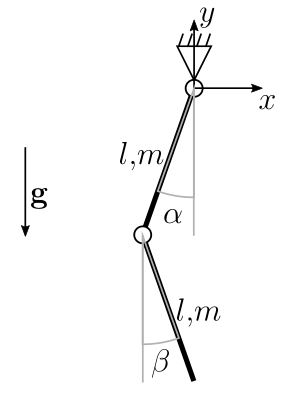
\includegraphics[width= 3cm]{tikz/02_02_2018_2a}
\end{figure}
\newline 
Dieses Doppelpendel besitzt zwei Freiheitsgrade. Die geeignete Wahl für die generalisierten Koordinaten lautet
\[
	\textbf{q} = \begin{bmatrix}
		\alpha \\
		\beta 
	\end{bmatrix}
\]
b) \\ \\
Die beiden Ortsvektoren zu den Schwerpunkten der Pendelstäbe lauten
\begin{align*}
	\textbf{a} = \frac{l}{2} \begin{bmatrix}
		\sin(\alpha) \\
		-\cos(\alpha)
	\end{bmatrix}
	\\
	\textbf{b} = \frac{l}{2}\begin{bmatrix}
		\sin(\beta) \\
		-\cos(\beta)
	\end{bmatrix}
	+ l \begin{bmatrix}
		\sin(\alpha) \\
		-\cos(\alpha)
	\end{bmatrix}
\end{align*}
c)\\ \\
Die Formel für das Massenträgheitsmoment kann aus der Formelsammlung entnommen werden. Dieses lautet daher
\[	
	\varTheta = \int_{-\frac{l}{2}}^{\frac{l}{2}}r^2\text{d}m = \frac{m}{l}\int_{-\frac{l}{2}}^{\frac{l}{2}}r^2\text{d}r = \frac{ml^2}{12}
\]
Die notwendigen Zeitableitungen, die später für die kinetische Energie benötigt werden lauten 
\begin{align*}
	\dot{\textbf{a}} &= \frac{l\dot{\alpha}}{2}\begin{bmatrix}
		\cos(\alpha) \\
		\sin(\alpha)
	\end{bmatrix}
	\\
	\dot{\textbf{b}} &= \frac{l\dot{\beta}}{2}\begin{bmatrix}
		\cos(\beta) \\
		\sin(\beta)
	\end{bmatrix}
	+ l\dot{\alpha}\begin{bmatrix}
		\cos(\alpha) \\
		\sin(\alpha)
	\end{bmatrix}
\end{align*}
Die Betragsquadrate dieser Vektoren lauten
\begin{align*}
	||\dot{\textbf{a}}||_2^2 &= \frac{l^2\dot{\alpha}^2}{4} \\
	||\dot{\textbf{b}}||_2^2 &= \left(\frac{l\dot{\beta}}{2}\cos(\beta) + l\dot{\alpha}\cos(\alpha)\right)^2 + \left(\frac{l\dot{\beta}}{2}\sin(\beta) + l\dot{\alpha}\sin(\alpha)\right)^2 \\
	&= \frac{l^2\dot{\beta}^2}{4}\cos^2(\beta) + l^2\dot{\beta}\dot{\alpha}\cos(\alpha)\cos(\beta) + l^2\dot{\alpha}^2\cos^2(\alpha) + \frac{l^2\dot{\beta}^2}{4}\sin^2(\beta) + l^2\dot{\beta}\dot{\alpha}\sin(\alpha)\sin(\beta) + l^2\dot{\alpha}^2\sin^2(\alpha) \\
	&= \frac{l^2\dot{\beta}^2}{4} + l^2\dot{\alpha}^2 + l^2\dot{\alpha}\dot{\beta}\cos(\alpha - \beta)
\end{align*}
Somit lautet die kinetische Energie
\begin{align*}
	T &= \frac{1}{2}m\left(\frac{l^2\dot{\alpha}^2}{4} + \frac{l^2\dot{\beta}^2}{4} + l^2\dot{\alpha}^2 + l^2\dot{\alpha}\dot{\beta}\cos(\alpha - \beta)\right) \\
	&= ml^2\left(\frac{2}{3}\dot{\alpha}^2 + \frac{1}{6}\dot{\beta} + \frac{1}{2}l^2\cos(\alpha - \beta)\dot{\alpha}\dot{\beta}\right)	
\end{align*}
e)\\ \\
Die potentielle Energie des Gesamtsystems lautet
\begin{align*}
	V &= -mg\frac{l}{2}\cos(\alpha) - mg\left(\frac{l}{2}\cos(\beta) + l\cos(\alpha)\right) \\
	  &= -\left(\frac{3}{2}\cos(\alpha) + \frac{1}{2}\cos(\beta)\right)
\end{align*}
e)\\ \\
Mit der Lagrange-Funktion und der Formel für den Euler-Lagrange-Formalismus folgt
\[
	\frac{\text{d}}{\text{d}t}\frac{\partial}{\partial \dot{\textbf{q}}}T = -\frac{\partial}{\partial \textbf{q}}V + \textbf{f}_e^T\left(\frac{\partial \textbf{a}}{\partial \textbf{q}} + \frac{\partial \textbf{b}}{\partial \textbf{q}}\right)
\]
Betrachtet man nun den Fall $V = 0$ muss die Erdbeschleunigung als externe Kraft angesetzt werden.
\[
	\textbf{f}_e = \begin{bmatrix}
		0  \\
		-mg
	\end{bmatrix}
\]
\newpage
\noindent
Nun müssen die gezeigt das die beiden Bedingungen aus den Euler-Lagrange-Formalismus
\[
	-\frac{\partial V}{\partial \alpha} = \textbf{f}_e^T\left(\frac{\partial \textbf{a}}{\partial \textbf{q}} + \frac{\partial \textbf{b}}{\partial \textbf{q}}\right) \quad \text{und} \quad -\frac{\partial V}{\partial \beta} = \textbf{f}_e^T\left(\frac{\partial \textbf{a}}{\partial \textbf{q}} + \frac{\partial \textbf{b}}{\partial \textbf{q}}\right) = \textbf{f}_e^T\frac{\partial \textbf{b}}{\partial \beta}
\]
Durch die Ermittlung dieser vier Terme sieht man
\begin{align*}
		-\frac{\partial V}{\partial \alpha} &= -\frac{3mgl}{2}\sin(\alpha) \\
		\textbf{f}_e^T\left(\frac{\partial \textbf{a}}{\partial \textbf{q}} + \frac{\partial \textbf{b}}{\partial \textbf{q}}\right) &= -mg\frac{3l}{2}\sin(\alpha)
\end{align*}
und
\begin{align*}
	-\frac{\partial V}{\partial \beta} &= -\frac{mgl}{2}\sin(\beta) \\
	\textbf{f}_e^T\frac{\partial \textbf{b}}{\partial \beta} &= -mg\frac{l}{2}
\end{align*}
	\textbf{Beispiel 3}\\ \\
a)\\ \\
Bei dieser RC-Ersatzschaltung wurden die Wärmeübergänge als Widerstände, konstante Temperaturen als Spannungsquellen
und veränderliche Temperaturen als Kapazitäten dargestellt.
\begin{figure}[h]
	\centering
	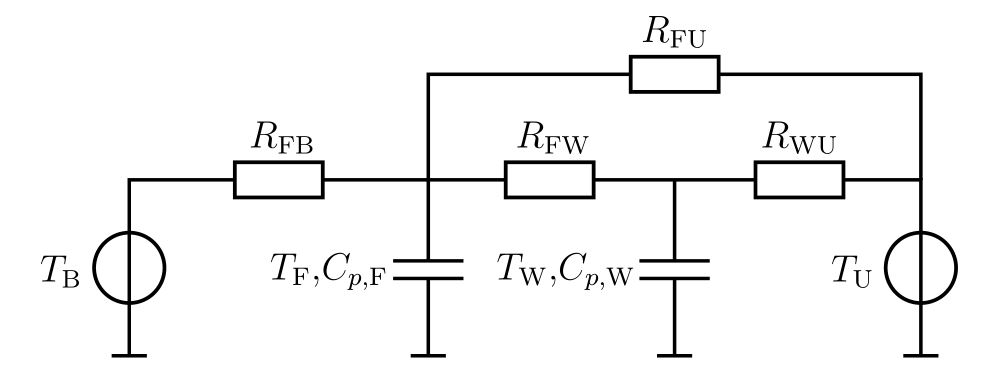
\includegraphics[width= 10cm]{tikz/02_02_2018_3a}
\end{figure}
\newline
b)\\ \\
Aus der RC-Ersatzschaltung ergeben sich folgende Differentialgleichungen
\begin{align*}
	C_{p,F}\frac{\text{d}}{\text{d}t}T_F(t) &= \frac{T_B - T_F(t)}{R_{FB}} + \frac{T_W(t) - T_{F}(t)}{R_{FW}} + \frac{T_U - T_F(t)}{R_{FU}} \\
	C_{p,W}\frac{\text{d}}{\text{d}t}T_W(t) &= \frac{T_U - T_W(t)}{R_{WU}} + \frac{T_F(t) - T_W(t)}{R_{FW}}
\end{align*}
\newpage
\noindent
Im stationären Fall lauten die beiden Differentialgleichungen
\begin{align*}
	0 &= (T_{B,R} - T_{F,R})R_{FW}R_{FU} + (T_{W,R} - T_{F,R})R_{FB}R_{FU} + (T_{U,R} - T_{F,R})R_{FB}R_{FW} \\
	0 &= T_{B,R}R_{FW}R_{FU} + T_{W,R}R_{FB}R_{FU} - T_{F,R}(R_{FW}R_{FU} + R_{FB}R_{FU} + R_{FB}R_{FW}) + T_{U,R}R_{FB}R_{FW}
\end{align*}
und
\begin{align*}
	0 &= (T_{U,R} -  T_{W,R})R_{FW} + (T_{F,R} - T_{W,R})R_{WU} \\
	0&= -T_{W,R}(R_{FW} + R_{WU}) + T_{F,R}R_{WU} + T_{U,R}R_{FW}
\end{align*}
Dadurch erhält man
\begin{align*}
	\textbf{\text{0}} &= \begin{bmatrix}
		R_{FW}R_{FU} & R_{FB}R_{FU} \\
		0 & -R_{FW} - R_{WU}
	\end{bmatrix}
	\begin{bmatrix}
		T_{B,R} \\
		T_{W,R}
	\end{bmatrix} \\
	&-
	\begin{bmatrix}
		R_{FW}R_{FU} + R_{FB}R_{FU} + R_{FB}R_{FW} & -R_{FB}R_{FW} \\
		-R_{WU} & -R_{FW}
	\end{bmatrix}
	\begin{bmatrix}
		T_{F,R} \\
		T_{U,R}
	\end{bmatrix}
\end{align*}
Durch Lösen dieses Gleichungssystem lautet die gesuchte Lösung
\begin{align*}
	T_{B,R} &= \frac{R_{FB}R_{FU} + R_{FB}R_{FW} + R_{FB}R_{WU} + R_{FU}R_{FW} + R_{FU}R_{WU}}{R_{FU}(R_{FW} + R_{WU})}T_{F,R} \\
	&- \frac{R_{FB}R_{FU} + R_{FB}R_{FW} + R_{FB}R_{WU}}{R_{FU}(R_{FW} + R_{WU})}T_{U,R}
\end{align*}
	\textbf{Beispiel 4}\\ \\
a)\\ \\
Die Sichtfaktormatrix muss folgende Form haben
\[
	\textbf{F} = \begin{bmatrix}
		F_{w,w} & F_{w,th} \\
		F_{th,w} & F_{th,th}
	\end{bmatrix}
\]
Mit den Faktoren
\begin{align*}
	F_{w,w} = 1 \qquad F_{w,th} = 0 \\
	F_{th,w} = 1  \qquad F_{th,th} = 0
\end{align*}
b)\\ \\
Durch Einsetzen folgt aus
\[
	\dot{\textbf{q}} = (\textbf{E} - \textbf{F})(\textbf{E} - (\textbf{E} - \text{diag}\{\varepsilon\})\textbf{F})^{-1}\text{diag}\{\varepsilon\}\sigma\textbf{T}^4
\]
folgende Nettowärmestromdichte
\begin{align*}
	\begin{bmatrix}
		\dot{q}_{w,s} \\
		\dot{q}_{th,s}
	\end{bmatrix}
	=
	\begin{bmatrix}
		0 & 0 \\
		-1 & 1
	\end{bmatrix}
	 \left(
	 	\begin{bmatrix}
	 		1 & 0 \\
	 		0 & 1
	 	\end{bmatrix}
	 	-
	 	\begin{bmatrix}
	 		1 - \varepsilon_w & 0 \\
	 		0 & 1 - \varepsilon_{th}
	 	\end{bmatrix}
	 	\cdot
	 	\begin{bmatrix}
	 		1 & 0 \\
	 		1 & 0
	 	\end{bmatrix}
	 \right)^{-1}
	 \begin{bmatrix}
	 	\varepsilon_w & 0 \\
	 	0 & \varepsilon_{th}
	 \end{bmatrix}
	 \sigma\begin{bmatrix}
	 	T_w^4 \\
	 	T_{th}^4
	 \end{bmatrix}
\end{align*}
\newpage
\noindent
\begin{align*}
	\begin{bmatrix}
	\dot{q}_{w,s} \\
	\dot{q}_{th,s}
	\end{bmatrix}
	&=
	\begin{bmatrix}
	0 & 0 \\
	-1 & 1
	\end{bmatrix}
	\left(
		\begin{bmatrix}
			1 & 0 \\
			0 & 1
		\end{bmatrix}
		-
		\begin{bmatrix}
			1 - \varepsilon_w & 0 \\
			1 - \varepsilon_{th} & 0
		\end{bmatrix}
	\right)^{-1}
	\begin{bmatrix}
	\varepsilon_w & 0 \\
	0 & \varepsilon_{th}
	\end{bmatrix}
	\sigma\begin{bmatrix}
	T_w^4 \\
	T_{th}^4
	\end{bmatrix}
	\\ \\
	\begin{bmatrix}
	\dot{q}_{w,s} \\
	\dot{q}_{th,s}
	\end{bmatrix}
	&=
		\begin{bmatrix}
	0 & 0 \\
	-1 & 1
	\end{bmatrix}
	\begin{bmatrix}
		\varepsilon_w & 0 \\
		\varepsilon_{th} - 1 & 0 
	\end{bmatrix}^{-1}
	\begin{bmatrix}
	\varepsilon_w & 0 \\
	0 & \varepsilon_{th}
	\end{bmatrix}
	\sigma\begin{bmatrix}
	T_w^4 \\
	T_{th}^4
	\end{bmatrix}
	\\ \\
		\begin{bmatrix}
	\dot{q}_{w,s} \\
	\dot{q}_{th,s}
	\end{bmatrix}
	&=
	\begin{bmatrix}
	0 & 0 \\
	-1 & 1
	\end{bmatrix}
	\frac{1}{\varepsilon_w}
	\begin{bmatrix}
		1 & 0 \\
		1 - \varepsilon_{th} & \varepsilon_w
	\end{bmatrix}
	\begin{bmatrix}
		\sigma\varepsilon_wT_w^4 \\
		\sigma\varepsilon_{th}T_{th}^4
	\end{bmatrix} 
	\\ \\
		\begin{bmatrix}
	\dot{q}_{w,s} \\
	\dot{q}_{th,s}
	\end{bmatrix}
	&=
	\begin{bmatrix}
	0 & 0 \\
	-1 & 1
	\end{bmatrix}
	\begin{bmatrix}
		\sigma T_w^4 \\
		(1 - \varepsilon_{th})\sigma T_{th}^4 + \sigma \varepsilon_{th}T_{th}^4
	\end{bmatrix}
	\\ \\
		\begin{bmatrix}
	\dot{q}_{w,s} \\
	\dot{q}_{th,s}
	\end{bmatrix}
	&=
	\begin{bmatrix}
		0 \\
		\varepsilon_{th}\sigma(T_{th}^4 - T_w^4)
	\end{bmatrix}
\end{align*}
c)\\ \\
Aufgrund der Konvektion folgt 
\[
	\dot{q}_{th,k} = \alpha_{th}(T_{th} - T_{Luft})
\]
d)\\ \\
Es muss natürlich 
\[
	\dot{q}_{th,k} + \dot{q}_{th,s} = 0
\]
woraus man auf
\[
	\alpha_{th}(T_{th} - T_{Luft}) + \varepsilon_{th}\sigma(T_{th}^4 - T_w^4) = 0
\]
Durch Umformen erhält man schließlich
\[
	T_{luft} = T_{th} + \frac{\varepsilon_{th}\sigma}{\alpha_{th}}(T_{th}^4 - T_w^4)
\]
e)\\ \\
Um einen geringeren Störeinfluss zu gewährleisten, muss entweder die Emmissivität des Thermometers $\varepsilon_{th}$ verringert oder der Wärmeübergangskoeffizient $\alpha_{th}$ erhöht werden. Ersteres kann durch die Wahl eines geeigneten Materials für die Thermometeroberfläche erreicht werden. Um den Wärmeübergangskoeffizient zu erhöhen muss die Umströmung des Thermometers verändert werden. Man könnte versuchen, in der Umgebung des Thermometers turbulente Strömungsverhältnisse zu erzeugen, da im turbulenten Bereich der Wärmeübergangskoeffizient höher ist als im laminaren.
	
	\newpage
	\subsection{16.03.2018}
	\textbf{Beispiel 1}\\ \\
a)\\ \\
Die gesuchte Masse lautet
\begin{align*}
	m_2 &= \int_{0}^{T}\int_{0}^{L}\int_{0}^{\tan(\alpha)x}\rho_2 \,\, \text{d}y\text{d}x\text{d}z \\
	&= \int_{0}^{T}\int_{0}^{L}\rho_2\tan(\alpha)x \,\, \text{d}x\text{d}z \\
	&= \int_{0}^{T}\rho_2\tan(\alpha)\frac{L^2}{2} \,\, \text{d}z \\
	&= \frac{1}{2}\rho_2L^2T\tan(\alpha)
\end{align*}
Der Schwerpunkt lautet
\begin{align*}
	s_x &= \frac{\int_{0}^{T}\int_{0}^{L}\int_{0}^{\tan(\alpha)x}x\rho_2 \,\, \text{d}y\text{d}x\text{d}z}{m_2} \\
	    &= \frac{\frac{1}{3}\rho_2L^2T\tan(\alpha)}{\frac{1}{2}\rho_2L^2T\tan(\alpha)} = \frac{2}{3}L \\ \\
	s_y &= \frac{\int_{0}^{T}\int_{0}^{L}\int_{0}^{\tan(\alpha)x}y\rho_2 \,\, \text{d}y\text{d}x\text{d}z}{m_2} \\
	    &= \frac{\frac{1}{2}\frac{1}{3}\rho_2L^3T\tan^2(\alpha)}{\frac{1}{2}\rho_2L^2T\tan(\alpha)} = \frac{1}{3}\tan(\alpha)L
\end{align*}
b)\\ \\
Freigeschnittene Körper:
\begin{figure}[h]
	\centering
	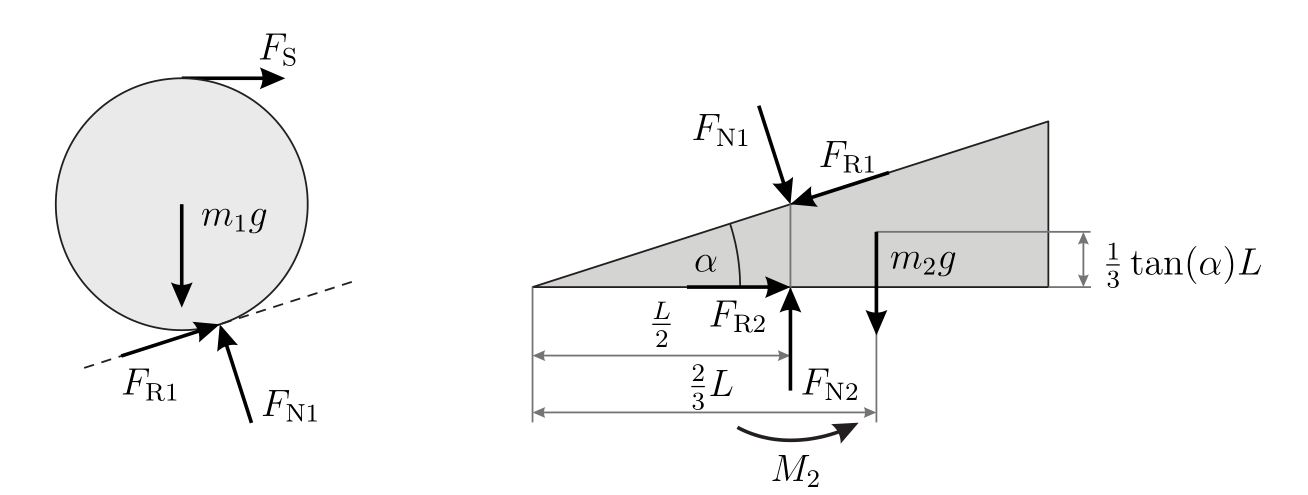
\includegraphics[width= 12.5cm]{tikz/16_03_2018_1b}
\end{figure}
\newpage
\noindent
c)\\ \\
Die geforderten Gleichgewichtsgleichungen lauten für die Walze
\begin{align*}
	\textbf{e}_x &: F_{R1}\cos(\alpha) + F_s - F_{N1}\sin(\alpha)\\
	\textbf{e}_y &: -m_1g + F_{R1}\sin(\alpha) + F_{N1}\cos(\alpha)\\
	\textbf{e}_z &: -rF_S + rF_{R1}
\end{align*}
und den Keil
\begin{align*}
	\textbf{e}_x &: F_{R2} - F_{R1}\cos(\alpha) + F_{N1}\sin(\alpha)\\
	\textbf{e}_y &: F_{N2} - m_2g - F_{R1}\sin(\alpha) - F_{N1}\cos(\alpha)
\end{align*}
d)\\ \\
Durch umformen dieser Gleichungen folgt für die gesuchten Kräfte
\begin{align*}
	F_{N1} &= m_1g & F_{N2} &= m_1g + m_2g \\
	F_{R1} &= m_1g\frac{\sin(\alpha)}{1+\cos(\alpha)} & F_{R2} &= -m_1g\frac{\sin(\alpha)}{1+\cos(\alpha)} \\
	F_S &= m_1g\frac{\sin(\alpha)}{1+\cos(\alpha)}
\end{align*}
e)\\ \\
Da es sich um Haftreibung handelt muss für Haftreibungskoeffizienten
\[
	\mu_1 > \frac{F_{R1}}{F_{N1}}, \quad \mu_2 > \frac{F_{R2}}{F_{N2}}
\]
	\textbf{Beispiel 2}\\ \\
a)\\ \\
Mithilfe des Satz von Steiner lautet das gesuchte Massenträgheitsmoment
\[
	I_d = I_s + ml_s^2
\]
b)\\ \\
In der Ruhelage lautet die gesuchte Länge
\[
	l_f = \sqrt{l_1^2 + l_{f,0}^2}
\]
Durch die Drehung um den Winkel $\varphi$ ergibt sich
\[
	l_f(\varphi) = \sqrt{l_1^2(1 - \cos(\varphi)^2) + (l_{f0} + l_1\sin(\varphi))^2}
\]
\newpage
\noindent
Somit folgt für den Winkel $\alpha_f(\varphi)$
\[
	\alpha_f(\varphi) = \arctan\left(\frac{l_1(1 - \cos(\varphi))}{l_{f0} + l_1\sin(\varphi)}\right)
\]
c)\\ \\
Der Drehimpulserhaltungssatz für die Wippe lautet hier
\begin{align*}
	I_d\ddot{\varphi} = - mgl_s\cos(\varphi) - k(l_f - l_{f0})(\sin(\alpha_f)\sin(\varphi) + \cos(\alpha_f)\cos(\varphi)) - d\dot{\varphi}l_2^2\cos^2(\varphi)
\end{align*}
d)\\ \\
Die gesamte im System gespeicherte Energie entspricht
\[
	E_{ges} = mgl_s\sin(\varphi) + \frac{1}{2}I_d\dot{\varphi}^2 + \frac{1}{2}k(l_f - l_{f0})^2
\]
	\textbf{Beispiel 3}\\ \\
a)\\ \\
RC-Ersatzschaltung:
\begin{figure}[h]
	\centering
	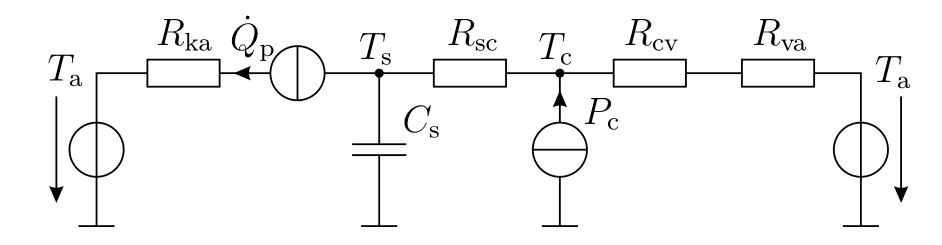
\includegraphics[width= 10cm]{tikz/16_03_2018_3a}
\end{figure}
\newline
Die Widerstände stellen die Wärmeübergänge, die Kapazität die Bereiche mit veränderlichen Temperaturen, die Stromquellen die Wärmeströme und die Spannungsquellen die konstanten Temperaturen dar.\\ \\
b)\\ \\
Die Chiptemperatur kann direkt aus der Ersatzschaltung bestimmt werden und lautet somit
\begin{align*}
	T_c(t) &= T_s(t) + \dot{Q}_{sc}R_{sc} = T_s(t) + \left(P_c + \frac{T_a - T_c(t)}{R_{cv} + R_{va}}\right)R_{sc}
\end{align*}
Durch Umformen erhält man
\[
	T_c(t) = \frac{T_s(t)(R_{cv} + R_{va}) + T_aR_{sc} + P_c(R_{cv} + R_{va}R_{sc})}{R_{sc} + R_{cv} + R_{va}}
\]
c)\\ \\
Die Temperaturänderung erfolgt nur durch die Wärmeströme über die Kapazität. Daher lautet die Differentialgleichung
\[
	\frac{\text{d}}{\text{d}t}T_s(t) = \frac{1}{C_s}(\dot{Q}_{sc} - \dot{Q}_p) =  \frac{1}{C_s}\left(P_c + \frac{T_a - T_c(t)}{R_{cv} + R_{va}} + \dot{Q}_p\right)
\]
\newpage
\noindent
d)\\ \\
Im stationären Fall verfällt die zeitliche Änderung, dadurch wird die Kapazität eine Unterbrechung und es ergibt sich für die gesuchten Temperaturen
\begin{align*}
	T_{c,\infty} &= T_a - (\dot{Q}_p - P_c)(R_{cv} + R_{va}) \\
	T_{s,\infty} &= T_{c,\infty} - R_{sc}\dot{Q}_p
\end{align*}
Diese Gleichungen wurden mithilfe der Ersatzschaltung aufgestellt. \\ \\
	\textbf{Beispiel 4}\\ \\
a)\\ \\
Die Wärmestromdichten lauten im stationären Betrieb
\[
	\dot{q}_s = \frac{P}{A_s} \quad;\quad \dot{q}_i = \frac{P}{A_i} \quad;\quad \dot{q}_a = \frac{P}{A_a}
\]
b)\\ \\
Aufgrund der angenommener Konvektion(Form aus der Formelsammlung) ergibt sich für die Außentemperatur
\[
	T_a = T_\infty + \frac{\dot{q}_a}{\alpha} = T_\infty + \frac{P}{A_a\alpha}
\]
c)\\ \\
Die Form der allgemeinen Wärmeleitgleichung für Zylinderkoordinaten ist in der Formelsammlung ersichtlich. Dadurch das die stationäre Wärmeleitgleichung benötigt vereinfacht sich die allgemeine Form zu
\[
	0 = \frac{\partial}{\partial r}\left(r^2\frac{\partial T(r)}{\partial r}\right)
\]
Mit den Randbedingungen
\[
	T(r_i) = T_i \quad,\quad T(r_a) = T_a
\]
d) \\ \\
Durch Lösen dieser Differentialgleichung erhält man die beiden Ansätze
\[
	\frac{\partial T(r)}{\partial r} = \frac{c_1}{r^2} \quad;\quad T(r) = -\frac{c_1}{r} + c_2
\]
Durch Einsetzen der Randbedingungen folgt die beiden Konstanten 
\[
	c_1 = \frac{T_i - T_a}{\frac{1}{r_a} - \frac{1}{r_i}} \quad;\quad c_2 = T_i + \frac{T_i - T_a}{\frac{1}{r_a} - \frac{1}{r_i}}\frac{1}{r_i}
\]
Somit lautet schließlich die gesuchte Temperatur
\[
	T_R = T_i + \frac{T_i - T_a}{\frac{1}{r_a} - \frac{1}{r_i}}\left(\frac{1}{r_i} - \frac{1}{r}\right)
\]
e)\\ \\
Die Bedingung am Innenrand lautet
\[
	\frac{\partial T(r)}{\partial r}\Biggl|_{r = r_i} = \frac{T_i - T_a}{\frac{1}{r_a} - \frac{1}{r_i}}\frac{1}{r_i^2} = -\frac{\dot{q}_i}{\lambda} = -\frac{P}{A_i\lambda}
\]
Formt man dieses um erhält man schließlich
\[
	T_i = T_a - \frac{Pr_i^2\left(\frac{1}{r_a} - \frac{1}{r_i}\right)}{A_i\lambda}
\]
f) \\ \\
Sämtliche Sichtfaktoren wurden durch die Summationsregel und dem Reziprozitätsgesetz bestimmt. Der einfachste Sichtfaktor zu bestimmen ist jener von Strahler auf Strahler, den dieser ist gleich 0 da der Strahler nicht auf sich selbst strahlt. Mit diesem Sichtfaktor und den genannten Regeln ergibt sich für die Sichtfaktormatrix
\[
	\textbf{F} = \begin{bmatrix}
		0 & 1 \\
		\frac{A_s}{A_i} & 1 - \frac{A_s}{A_i}
	\end{bmatrix}
\]
g)\\ \\
Durch Anwendung der Form der Nettowärmestromdichte aus der Formelsammlung ergibt sich diese
\[
	\begin{bmatrix}
		\dot{q}_s \\
		\dot{q}_i
	\end{bmatrix}
	=
	\begin{bmatrix}
		\sigma(T_s^4 - T_i^4) \\
		\sigma\frac{A_s}{A_i}(-T_s^4 + T_i^4)
	\end{bmatrix}
\]
Für schwarze Strahler gilt $\varepsilon = 1$. \\ \\
h) \\ \\ 
Formt die erste Zeile der Nettowärmestromdichte auf die Strahlertemperatur um folgt für diese
\[
	T_s = \sqrt[4]{T_i^4 + \frac{\dot{q}_s}{\sigma}} = \sqrt[4]{T_i^4 + \frac{P}{A_s}\sigma}
\]
	
	\newpage
	\subsection{18.05.2018}
	\textbf{Beispiel 1}\\ \\
a)\\ \\
Die gesuchte Differentialgleichung kann mithilfe der Energieerhaltung aufgestellt werden und lautet daher
\[
	\rho c_pl_chd\left(\frac{\partial T}{\partial t}\right) = P - \dot{Q}
\]
Der Wärmestrom $\dot{Q}$ besitzt ein negatives Vorzeichen, da dieser aus dem Chip austritt.\\ \\
b)\\ \\
Die gesuchte Temperatur lautet im stationären Zustand
\[
	T_0 = \frac{P}{dh}\left(kl_w  - \frac{l_w^3}{3} + \frac{l_k}{\lambda_k} + \frac{1}{\alpha_{wk}} + \frac{1}{\alpha_{ku}}\right) + T_\infty
\]
Diese Gleichung erhält man durch Umformen un der Formel \textit{Wärmestromdichte und Wärmeübergangskoeffizient bei mehrschichtigen Wandaufbau} aus der Formelsammlung.\\ \\
c)\\ \\
Die maximale Wärmeleistung pro Chipfläche lautet
\[
	p_{max} = \frac{1}{k}\left(\frac{\partial T_w(x)}{\partial x}\right)_{\text{max}}
\]
Durch den gegebenen Temperaturgradienten lässt sich diese auf
\[
	p_{max} = \frac{G}{k}
\]
vereinfachen.
	\textbf{Beispiel 2}\\ \\
a)\\ \\
Freigeschnittene Teilkörper:
\begin{figure}[h]
	\centering
	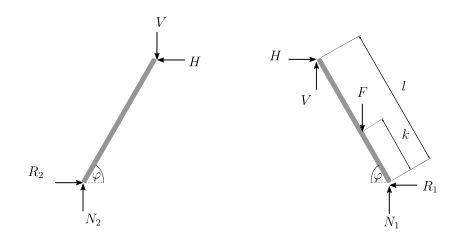
\includegraphics[width= 8cm]{tikz/18_05_2018_2a}
\end{figure}
\newpage
\noindent
b)\\ \\
Die notwendigen Gleichgewichtsgleichungen lautet für den rechten Teil 
\begin{align}
	\textbf{e}_x &: R_1 = H\\
	\textbf{e}_y &: F = V + N_1\\
	\textbf{e}_z &: k\cos(\varphi)F = Vl\cos(\varphi) + Hl\sin(\varphi)
\end{align}
und den linken Teil
\begin{align*}
	\textbf{e}_x &: R_2 = H\\
	\textbf{e}_y &: N_2 = V\\
	\textbf{e}_z &: Hl\sin(\varphi) = Vl\cos(\varphi)
\end{align*}
Durch gezieltes Umformen dieser Gleichung erhält man für die Bodenkontaktkräfte
\begin{align*}
	R &= F\frac{k}{2l\tan(\varphi)} \\
	N_1 &= F\frac{2l - k}{2l} \\
	N_2 &= F\frac{k}{2l}
\end{align*}
c)\\ \\
Da es sich um Haftreibung handelt lautet die Bedingung für den rechten Teil
\begin{align*}
	\mu \geq \frac{R_1}{N_1} &= \frac{F\frac{k}{2l\tan(\varphi)}}{F\frac{2l - k}{2l}} = \frac{k}{(2l - k)\tan(\alpha)}
\end{align*}
und den linken Teil
\[
	\mu \geq \frac{R_2}{N_2} = \frac{F\frac{k}{2l\tan(\varphi)}}{F\frac{k}{2l}} = \frac{1}{\tan(\alpha)}
\]
	\newpage
\noindent
\textbf{Beispiel 3}\\ \\
a)\\ \\
Die beiden gesuchten Ortsvektoren lauten
\begin{align*}
	\textbf{r}_{S_g} &= \begin{bmatrix}
		a\sin(\varphi_g) \\
		-a\cos(\varphi_g) \\
		0					
	\end{bmatrix}
	\\ \\
	\textbf{r}_{S_k} &= \begin{bmatrix}
		l\sin(\varphi_g) + b\sin(\varphi_k) \\
		-\cos(\varphi_g) - b\cos(\varphi_k) \\
		0
	\end{bmatrix}
\end{align*}
Die zugehörigen Geschwindigkeitsvektoren lauten
\begin{align*}
	\dot{\textbf{r}}_{S_g} &= \begin{bmatrix}
		a\cos(\varphi_g)\omega_g \\
		a\sin(\varphi_g)\omega_g \\
		0
	\end{bmatrix}
	\\ \\
	\dot{\textbf{r}}_{S_k} &= \begin{bmatrix}
		l\omega_g\cos(\varphi_g) + b\omega_k\cos(\varphi_k) \\
		l\omega_g\sin(\varphi_g) + b\omega_k\cos(\varphi_k) \\
		0
	\end{bmatrix}
\end{align*}
b)\\ \\
Die benötigten Zwischenberechnung ergeben
\begin{align*}
	||\dot{\textbf{r}}_{S_g}||_2^2 &= a^2\omega^2_g \\
	||\dot{\textbf{r}}_{S_k}||_2^2 &= (l\omega_g\cos(\varphi_g) + b\omega_k\cos(\varphi_k))^2 + (l\omega_g\sin(\varphi_g) + b\omega_k\cos(\varphi_k))^2 \\
	&= l^2\omega^2_g + b^2\omega^2_k  + 2lb\omega_g\omega_k\cos(\varphi_g - \varphi_k)
\end{align*}
c)\\ \\
Die beiden Komponenten der kinetischen Energie lautet
\begin{align*}
	T_{tran} &= \frac{m_g}{2}a^2\omega^2_g + \frac{m_k}{2}\left(2lb\omega_g\omega_k\cos(\varphi_g - \varphi_k)\right) \\
	T_{rot} &= \frac{\varTheta_g}{2}\omega^2_g + \frac{\varTheta_k}{2}\omega^2_k
\end{align*}
Zusätzlich lautet noch die potentielle Energie
\[
	V = -g\left[m_ga\cos(\varphi_g) + m_k(l\cos(\varphi_g) + b\cos(\varphi_k))\right]
\]
\newpage
\noindent
c)\\ \\
Um die Massenmatrix \textbf{M} zu bestimmen müssen Ableitung vorher durchgeführt werden die folgendes ergeben.
\begin{align*}
	\frac{\partial T}{\partial \omega_g} &= m_g a^2\omega_g + m_k\left(l^2\omega_g + bl\omega_k\cos(\varphi_g - \varphi_k)\right) + \varTheta_g\omega_g \\
	\frac{\text{d}}{\text{d}t}\frac{\partial T}{\partial \omega_g} &= m_ga^2\dot{\omega}_g + m_kl^2\dot{\omega}_g + m_kbl\dot{\omega}_k\cos(\varphi_g - \varphi_k) - m_klb\sin(\varphi_g - \varphi_k)(\omega_g - \omega_k) + \varTheta_g\dot{\omega}_g \\ \\
	\frac{\partial T}{\partial \omega_k} &= m_k\left(b^2\omega_k + 2lb\omega_g\cos(\varphi_g - \varphi_k)\right) + \varTheta_k\omega_k \\
	\frac{\text{d}}{\text{d}t}\frac{\partial T}{\partial \omega_k} &= m_k\left(b^2\dot{\omega}_k + lb\dot{\omega}_g\cos(\varphi_g - \varphi_k) - bl\omega_g\sin(\varphi_g - \varphi_k)(\omega_g - \omega_k)\right) + \varTheta_k\dot{\omega}_k
\end{align*}
Durch Koeffizientenvergleich mit 
\[
	\textbf{M}\ddot{\textbf{q}} 
\]
erhalten man für die Massenmatrix
\[
	\textbf{M} = \begin{bmatrix}
		m_ga^2 + m_kl^2 + \varTheta_g & m_klb\cos(\varphi_g - \varphi_k) \\
		m_klb\cos(\varphi_g - \varphi_k) & m_kb^2 + \varTheta_k
	\end{bmatrix}
\]
Der Vektor für die externe Kraft lautet
\[
	\textbf{F}_c = F-c\begin{bmatrix}
		\cos(\varphi_k) \\
		\sin(\varphi)_k
	\end{bmatrix}
\]
Der Ortsvektor zum Angriffspunkt dieser Kraft lautet wiederum
\[
	\textbf{r}_{f_c} = \begin{bmatrix}
		l\sin(\varphi_g) + \left(l_d + \frac{l_m}{2}\right)\sin(\varphi_k) \\
		l\cos(\varphi_g) + \left(l_d + \frac{l_m}{2}\right)\cos(\varphi_k)
	\end{bmatrix}
\]
Die notwendigen Ableitungen lauten
\[
	\frac{\partial \textbf{r}_{f_c}}{\partial \varphi_g} = \begin{bmatrix}
			l\cos(\varphi_g) \\
			l\sin(\varphi_g)
		\end{bmatrix}
		\quad,\quad
		\frac{\partial \textbf{r}_{f_c}}{\partial \varphi_k} = \begin{bmatrix}
			\left(l_d + \frac{l_m}{2}\right)\cos(\varphi_k) \\
			\left(l_d + \frac{l_m}{2}\right)\sin(\varphi_k)
			\end{bmatrix}
\]
Mit der Rechenvorschrift für die generalisierten Kräfte aus der Formelsammlung ergibt sich nun für den gesuchten Vektor
\[
	\tau = \begin{bmatrix}
		M_g + F_cl\cos(\varphi_g - \varphi_k) \\
		F_c\left(l_d + \frac{l_m}{2}\right)
	\end{bmatrix}
\]
d)\\ \\
Aus der gegebenen Bewegungsgleichung und der Tatsache, dass $\varphi_g = \varphi_k$ und $\omega_g = \omega_k$ die Bedingung
\[
	\frac{m_ga + m_kl}{m_{11} + m_{12}} = \frac{m_kb}{m_{21} + m_{22}}
\]
\newpage
\noindent
e)\\ \\
Durch Anwendung der Formel \textit{Schwerpunkt eines zusammengesetzten Körpers} aus der Formelsammlung folgt für den gesuchten Abstand
\[
	b = \frac{l_k^2r_i^2 + l_m(r_a^2 - r_i^2)(2l_d + l_m)}{2\left(r_i^2l_k + (r_a^2 - r_i^2)l_m\right)}
\]
f)\\ \\
Mithilfe des Satzes von Steiner ergibt sich für das gesuchte Massenträgheitsmoment
\[
	\varTheta_{m,zz}^{(S_k)} = \varTheta_{m,zz}^(S_m) + m_m\left(l_d + \frac{l_m}{2} - b\right)^2 
\]
mit der Masse
\[
	m_m = \rho_k\pi l_m(r_a^2 - r_i^2)
\]
g)\\ \\
Das gesuchte Massenträgheitsmoment lautet
\begin{align*}
	\int_{\mathcal{V}}\rho_k(x^2 + y^2)\,\text{d}x\text{d}y\text{d}z &= \int_{\mathcal{V}}\rho_k(r^3\cos^2(\varphi) + ry^2)\,\text{d}r\text{d}\varphi\text{d}y = 
	\int_{b - l_k}^{b}\int_{0}^{2\pi}\int_{0}^{r_i}\rho_k(r^3\cos^2(\varphi) + ry^2)\,\text{d}r\text{d}\varphi\text{d}y \\
	&= 	\int_{b - l_k}^{b}\int_{0}^{2\pi}\rho_k\left(\frac{1}{4}r_i^4\cos^2(\varphi) + \frac{1}{2}r_i^2y^2\right)\,\text{d}\varphi\text{d}y = 	\int_{b - l_k}^{b}\rho_k\left(\frac{1}{4}r_i^4\pi + \frac{1}{2}r_i^2 2\pi y\right)\, \text{d}y \\
	&= \rho_kr_i^2\pi l_k\left(\frac{1}{4}r_i + \frac{1}{3}(3b^2 - 3bl_k + l_k^2)\right) \\ \\
	\varTheta_{m,zz}^{(S_k)} &= \frac{1}{3}m_s(3b^2 - 3l_kb + l_k^2) + \frac{1}{4}m_sr_i^2
\end{align*}
mit $m_s = \rho_kr_i^2\pi l_k$ \\ \\
	\newpage
\noindent
\textbf{Beispiel 4}\\ \\
a)\\ \\
Die drei Sichtfaktoren, die die Strahlung auf sich selbst beschreiben lauten
\[
	F_{s1s1} = F_{s2s2} = F_{aa} = 0 
\]
da diese nicht auf sich selbst strahlen.
Die restlichen Sichtfaktoren wurden mit der Cross-String-Methode, der Summationsregel und dem Reziprozitätsgesetz bestimmt.
\begin{align*} 
	F_{s1a} &= \frac{3b - 2b}{2b} = \frac{1}{2} \\
	F_{s1s2} &= 1 - F_{s1a} - F_{s1s1} = \frac{1}{2} \\
	F_{s2s1} &= \frac{A_{s1}}{A_{s2}}F_{s1s2} = \frac{1}{4} \\
	F_{s2a} &= 1 - F_{s2s1} - F_{s2s2} = \frac{3}{4} \\
	F_{as2} &= \frac{A_{s2}}{A_a}F_{s2a} = \frac{3}{4} \\
	F_{as1} &= 1 - F_{as2} - F_{aa} = \frac{1}{4}
\end{align*}
Damit ergibt sich für die Sichtfaktormatrix
\[
	\textbf{F} = \begin{bmatrix}
		0 & \frac{1}{2} & \frac{1}{2} \\
		\frac{1}{4} & 0 & \frac{3}{4}\\
		\frac{1}{4} & \frac{3}{4} & 0
	\end{bmatrix}
\]
b)\\ \\
Durch Anwendung der Formel für die Nettowärmestromdichte und durch Umformen erhält man
\[
	\begin{bmatrix}
		\dot{q}_{s1} \\
		\dot{q}_{s2} \\
		\dot{q}_{a,0}
	\end{bmatrix}
	= \frac{\sigma}{16}
	\begin{bmatrix}
		14 + 2\varepsilon_a & -14 + 6\varepsilon_a & -8\varepsilon_a \\
		-7 + 3\varepsilon_a & 7 + 9\varepsilon_a & -12\varepsilon_a \\
		-4\varepsilon_a & -12\varepsilon_a & 16\varepsilon_a
	\end{bmatrix}
	\begin{bmatrix}
		T_{s1}^4 \\
		T_{s2}^4 \\
		T_a^4
	\end{bmatrix}
\]
c)\\ \\
Hier muss die Wärmeleitgleichung für kartesische Koordinaten angewendet werden. Da Temperatur nur räumlich von y abhängig ist lautet nun die Wärmeleitgleichung
\[
	c_a\rho_a\frac{\partial T_a}{\partial t} = - \lambda_a\frac{\partial^2T_a}{\partial y^2}
\]
mit den Randbedingungen
\begin{align*}
	T(-d,t) &= T_\infty \\
	\dot{q}_a(0,t) &= -\lambda_a\frac{\partial T_a}{\partial y} = \dot{q}_{a,0}
\end{align*}
\newpage
\noindent
d)\\ \\
Die allgemeine stationäre Lösung der Wärmeleitgleichung lautet
\begin{align*}
  - \lambda_a\frac{\partial^2T_a}{\partial y^2} &= 0\\
	 -\lambda_a \frac{\partial T_a}{\partial y} &= C_1 \\
	 -\lambda_a T_a &= C_1y + C_2
\end{align*}
Durch Einsetzen der Randbedingungen ergibt sich für die Konstanten
\begin{align*}
	C_1 &= \dot{q}_{a,0} \\
	C_2 &= \lambda T_\infty - \dot{q}_{a,0}d
\end{align*}
Dadurch lautet nun das Temperaturprofil
\[
	T = -\frac{\dot{q_{a,0}}}{\lambda_a}(y + d) + T_\infty
\]
	
	\subsection{13.07.2018}
	\textbf{Beispiel 1}\\ \\
Freigeschnittenen Stäbe:
\begin{figure}[h]
	\centering
	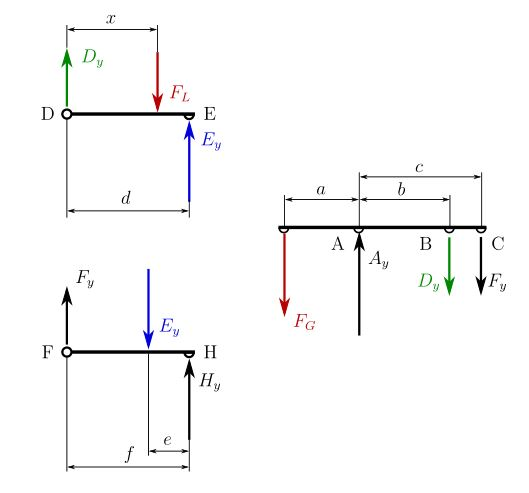
\includegraphics[width= 10cm]{tikz/13_07_2018_1}
\end{figure}
\newpage
\noindent
a)\\ \\
Die Gleichgewichtsgleichungen für den Stab D-E lauten
\begin{align*}
	\textbf{e}_y &: D_y + E_y - F_L = 0\\
	\textbf{e}_z &: E_yd - F_Lx = 0 
\end{align*}
Aus diesen folgen nun die Kräfte
\begin{align*}
	E_y &= F_L \frac{x}{d} \\
	D_y &= F_L \left(1 - \frac{x}{d}\right)
\end{align*}
b)\\ \\
Die Gleichgewichtsgleichungen für den Stab F-H lauten
\begin{align*}
	\textbf{e}_y &: F_y + H_y - E_y = 0\\
	\textbf{e}_z &: E_ye - F_yf = 0
\end{align*}
Aus diesen folgen nun die Kräfte
\begin{align*}
	F_y &= E_y \frac{e}{f} = F_L \frac{x}{d}\frac{e}{f} \\
	H_y &= E_y - F_y \\
		&= F_L \frac{x}{d}\left(1 - \frac{e}{f}\right)
\end{align*}
c)\\ \\
Die Gleichgewichtsgleichungen für den Stab A-B-C lauten
\begin{align*}
	\textbf{e}_y &: A_y - F_G - D_y - F_y = 0\\
	\textbf{e}_z &: F_Ga - D_yb - F_yc = 0
\end{align*}
Aus diesen folgen nun die Kräfte
\begin{align*}
	F_G &= D_y\frac{b}{a} + F_y\frac{c}{a} \\
		&= \frac{F_L}{a}\left[b - \frac{x}{d}\left(b - \frac{ec}{f}\right)\right] \\
	A_y &= F_L\left[\frac{b}{a} - \frac{x}{d}\left(\frac{b}{a} - \frac{ec}{af}\right) + 1 - \frac{x}{d}\left(1 - \frac{e}{f}\right)\right]
\end{align*}
d)\\ \\
Damit die geforderte Bedingung eingehalten werden kann, muss lautet das Längenverhältnis
\[
	\frac{b}{c} = \frac{e}{f}
\]
Dadurch gilt $F_G = F_L\frac{b}{a}$.
	\newpage
\noindent
\textbf{Beispiel 2} \\ \\
a)\\ \\
Dieses System besitzt folgende Freiheitsgrade
\[
	\textbf{q}^T = \begin{bmatrix}
		x_w & \varphi_1 & \varphi_2 & l_2
	\end{bmatrix}
\]
b)\\ \\
Die jeweiligen Ortsvektoren zu den Schwerpunkten lauten
\begin{align*}	
	\textbf{r}_W &= \begin{bmatrix}
		x_W \\
		0
	\end{bmatrix}
	\\
	\textbf{r}_{S1} &= \begin{bmatrix}
		x_w + \frac{l_1}{2}\sin(\varphi_1) \\
		-\frac{l_a}{2}\cos(\varphi_1)
	\end{bmatrix}
	\\
	\textbf{r}_M &= \begin{bmatrix}
		x_W + l_1\sin(\varphi_1) + l_2\sin(\varphi_2) \\
		-l_1\cos(\varphi_1) - l_2\cos(\varphi_2)
	\end{bmatrix}
\end{align*}
c)\\ \\
Die entsprechenden Geschwindigkeiten und Winkelgeschwindigkeiten der Schwerpunkte lauten
\begin{align*}
	\textbf{v}_W = \begin{bmatrix}
		\dot{x}_W \\
		0
	\end{bmatrix}
	\quad&,\quad
	\omega_W = 0
	\\
	\textbf{v}_{S1} = \begin{bmatrix}
		\dot{x}_W  +\frac{l_1}{2}\cos(\varphi_1)\dot{\varphi}_1 \\
		\frac{l_1}{2}\sin(\varphi_1)\dot{\varphi}_1
	\end{bmatrix}
	\quad&,\quad
	\omega_{S1} = \dot{\varphi}_1
	\\
	\textbf{v}_M = \begin{bmatrix}
		\dot{x}_W + l_1\cos(\varphi_1)\dot{\varphi}_1 + \dot{l}_2\sin(\varphi_2) + l_2\cos(\varphi_2)\dot{\varphi}_2 \\
		l_1\sin(\varphi_1)\dot{\varphi}_1 - \dot{l}_2\cos(\varphi_2) + l_2\sin(\varphi_2)\dot{\varphi}_2
	\end{bmatrix}
	\quad&,\quad
	\omega_M = \dot{\varphi}_2
\end{align*}
Die kinetischen Teilenergien des Systems lauten
\begin{align*}
	T_t &= \frac{1}{2}\textbf{v}^T_w\textbf{v}_W m_W + \frac{1}{2}\textbf{v}^T_{S1}\textbf{v}_{S1}m_1 + \frac{1}{2}\textbf{v}^T_M\textbf{v}_Mm_M \\
	T_r &= \frac{1}{2} \omega_1^2J_1
\end{align*}
Damit lautet die gesamte kinetische Energie des Systems
\[
	T = T_t + T_r
\]
\newpage
\noindent
d)\\ \\
Die potentielle Energie dieses Systems setzt sich aus der zusammen die in dem Stab + Masse und der in der Feder gespeichert wird zusammen. Diese beiden Teilenergien lauten
\begin{align*}
	V_m &= -m_1g\frac{l_1}{2}\cos(\varphi_1) - m_Mg\left(l_1\cos(\varphi_1) + l_2\cos(\varphi_2)\right) \\
	V_F &= \int_{x_0}^{x_W}F_F(\tilde{x})\,\text{d}\tilde{x} \\
		&= \frac{1}{2}c_1(x_W - x_0)^2 + \frac{1}{4}c_2(x_W - x_0)^4
\end{align*}
Somit ergibt sich für die gesamte potentielle Energie 
\[
	V = V_M + V_F
\]
f)\\ \\
Der Vektor für die generalisierten Kräfte setzt sich aus zwei Teilen zusammen. Den für den Waagen und den für die Punktmasse.
Für den Waagen gilt
\begin{align*}
	\textbf{F}_{an} = \begin{bmatrix}
		F_{an} \\
		0
	\end{bmatrix}
	\quad,\quad
	\textbf{r}_{an} = \begin{bmatrix}
		x_W \\
		0
	\end{bmatrix}
\end{align*}
Somit lautet dann der gesuchte Vektor für den Waagen
\begin{align*}
		\tau_{F_{an}} &= \left(\frac{\partial \textbf{r}_{F_{an}}}{\partial \textbf{q}}\right)^T \textbf{F}_{an} \\
		&= \begin{bmatrix}
			F_{an} & 0 & 0 & 0
		\end{bmatrix}^T
\end{align*}
Für die Punktmasse gilt
\[
	\textbf{F}_M = F_M\begin{bmatrix}
		-\sin(\varphi_2) \\
		\cos(\varphi_2)
	\end{bmatrix}
	\quad,\quad
	\textbf{r}_{F_M} = \begin{bmatrix}
		x_W + l_1\sin(\varphi_1) + l_2\sin(\varphi_2) \\
		-l_1\cos(\varphi_1) - l_2\cos(\varphi_2)
	\end{bmatrix}
\]
Somit lautet dann der gesuchte Vektor für die Punktmasse
\begin{align*}
	\tau_{F_M} &= \left(\frac{\partial \textbf{r}_{F_M}}{\partial \textbf{q}}\right)^T \textbf{F}_M \\
	&= F_M\begin{bmatrix}
		-\sin(\varphi_2) \\
		-l_1\sin(\varphi_2)\cos(\varphi_1) + l_1\cos(\varphi_2)\sin(\varphi_1) \\
		0 \\
		-1
	\end{bmatrix}
\end{align*}
Somit ergibt sich für den gesamten Vektor
\[
	\tau = \tau_{F_{an}} + 	\tau_{F_M}
\]
\newpage
\noindent
g)\\ \\
Die potentielle Energie wird sich nicht ändert wenn M nicht mehr als Punktmasse behandelt wird. Jedoch die kinetische Energie muss um den rotatorischen Teil der Masse M erweitert werden.
\[
	T_{M,r} = \frac{1}{2}\omega^2_MJ_2
\]
Die neue kinetische Energie des Systems lautet daher
\[
	T = T_t + T_r + T_{M,r} 
\]
h) \\ \\
Auf die Punktmasse M wirkenden Kräfte:
\begin{figure}[h]
	\centering
	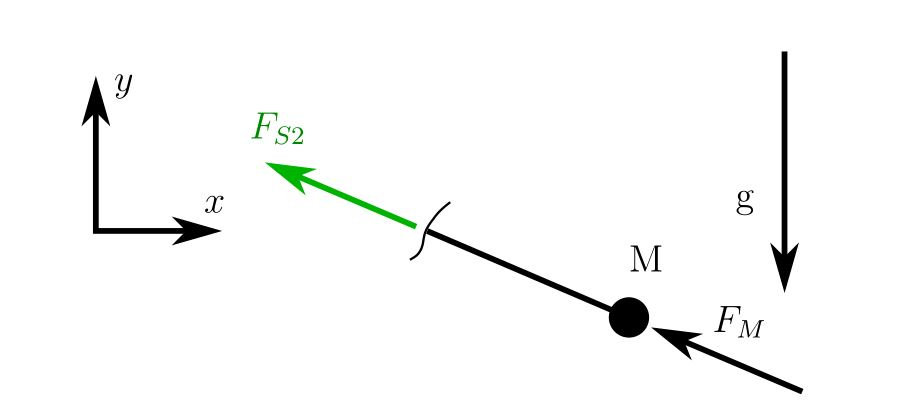
\includegraphics[width= 8cm]{tikz/13_07_2018_2h}
\end{figure}
\newline
Die Impulsbilanz ergibt mit der bekannten Geschwindigkeit
\[
	m_M\textbf{a}_M = \begin{bmatrix}
		F_{S2}\sin(\varphi_2) - F_M\sin(\varphi_2) \\
		F_{S2}\cos(\varphi_2) + F_M\cos(\varphi_2) - m_M
	\end{bmatrix}
\]
Durch Umformen dieser beiden Gleichungen, ergibt sich für die Stabkraft
\[
	F_{S2} = m_M\left(-a_{M,x}\sin(\varphi_2) + a_{M,y}\cos(\varphi_2)\right) - F_M + m_Mg\cos(\varphi_2)
\]
	\newpage
\noindent
\textbf{Beispiel 3}\\ \\
a) \\ \\
Der erste Sichtfaktor der leicht bestimmt werden kann, ist jener von Boden zu Boden. Dieser lautet
\[
	F_{BB} = 0
\]
da der Boden ja nicht auf sich selbst strahlt. Die restlichen drei Sichtfaktoren müssen mit der Summationsregel und dem Reziprozitätsgesetz bestimmt werden. Für diese gilt schließlich
\begin{align*}
	F_{BK} &= 1 - F_{BB} = 0 \\
	F_{KB} &= \frac{A_B}{A_K} \\
	F_{KK} &= 1 - F_{KB} = 1 - \frac{A_B}{A_K}
\end{align*}
Damit lautet die Sichtfaktormatrix
\[
	\textbf{F} = \begin{bmatrix}
		0 & 1 \\
		\frac{A_B}{A_K} & 1 - \frac{A_B}{A_K}
	\end{bmatrix}
\]
b) \\ \\
Durch Anwenden der Formel für die Nettowärmestromdichte und dem gegebenen Emissionskoeffizienten lautet die gesuchte Wärmestromdichte
\[
	\dot{q}_{B,s} = \varepsilon_B\sigma\left(T^4(t,d) - T_K^4\right)
\]
c) \\ \\
Die gesuchte Gesamtwärmestromdichte setzt sich aus der obigen Wärmestromdichte und derer durch Konvektion hervorgerufenen Wärmestromdichte zusammen und lautet
\[
	\dot{q}_B = \dot{q}_{B,s} + \alpha(T(d,t) - T_R)
\]
d) \\ \\
Die Differentialgleichung lautet für dieses Problem
\[
	\frac{\partial T(t,z)}{\partial t} = a\frac{\partial^2T(z,t)}{\partial z^2}
\]
Mit den Anfangs- und Randbedingungen
\begin{align*}
	T(0,z) &= T_0 \\
	\frac{\partial T(t,z)}{\partial z}\Biggl|_{t,z = d} = -\frac{\dot{q}_B(t)}{\lambda}
\end{align*}
Abhängig vom Heizungstyp ergeben sich die Bedingungen
\begin{align*}
	\frac{\partial T(t,z)}{\partial z}\Biggl|_{t,z = 0} = \frac{1}{\lambda}\frac{4P_{el}}{D^2\pi} \qquad \text{für elektrische Heizung} \\
	T(t,0) = T_W \qquad \text{für Warmwasserheizung}
\end{align*}
e)\\ \\
Durch die schlechtere Wärmleitfähigkeit würde sich auch der Wärmewiderstand des Fußboden vergrößern. Bei der elektrischen Heizung bleibt der Wärmestrom gleich, wird erst bei einem höheren Temperaturniveau in den Raum abgegeben. Bei der Warmwasserheizung wird der Wärmestrom sinken, die Heizschicht die konstante Temperatur $T_W$ hat.\\ \\
	\textbf{Beispiel 4}\\ \\
a)\\ \\
Zeichnung:
\begin{figure}[h]
	\centering
	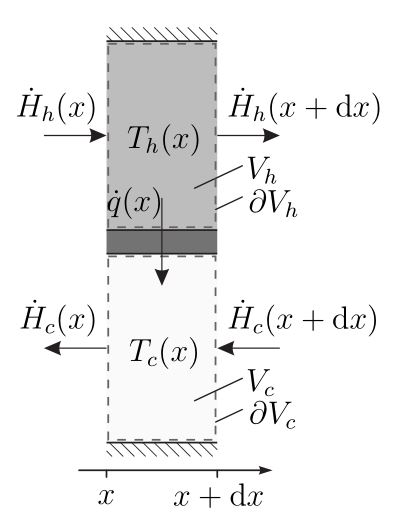
\includegraphics[width= 5cm]{tikz/13_07_2018_4a}
\end{figure}
\newline
Sämtliche Wärmeströme aus der Zeichnung lauten
\begin{align*}
	\dot{H}_h(x) &= \dot{m}_hc_pT_h(x) \\
	\dot{H}_h(x + \text{d}x) &= \dot{m}_hc_pT_h(x + \text{d}x) \\
	\dot{H}_c(x) &= \dot{m}_cc_pT_c(x) \\
	\dot{H}_c(x + \text{d}x) &= \dot{m}_cc_pT_c(x + \text{d}x) \\
	\dot{q}(x) &= kB(T_h(x) - T_c(x))
\end{align*}
b)\\ \\
Die beiden Energiebilanzen des Kontrollvolumen lauten
\begin{align*}
	\dot{m}_hc_pT_h(x) - \dot{m}_hc_pT_h(x + \text{d}x) - kB(T_h(x) - T_c(x))\text{d}x &= 0 \\
	\dot{m}_cc_pT_c(x) - \dot{m}_cc_pT_c(x + \text{d}x) - kB(T_h(x) - T_c(x))\text{d}x &= 0
\end{align*}
Durch Umformen erhält man die Differentialgleichungen
\begin{align*}
	\frac{\text{d}T_h(x)}{\text{d}t} &= \frac{kB}{\dot{m}_hc_p}\left(T_h(x) - T_c(x)\right) \\
	\frac{\text{d}T_c(x)}{\text{d}t} &= \frac{kB}{\dot{m}_cc_p}\left(T_h(x) - T_c(x)\right)
\end{align*}
c)\\ \\
Durch Lösen dieses Differentialgleichungssystem ergeben sich für die beiden Temperaturverläufe
\begin{align*}
	T_h(x) &= K \frac{T_{c,2} - T_{h,1}}{KL + 1}x + T_{h,1} \\
	T_c(x) &= T_h(x) - \frac{T_{c,2} - T_{h,1}}{KL + 1}
\end{align*}
mit
\[
	K = \frac{kB}{\dot{C}}
\]
Zu verwendende Formel zum Lösen befinden sich in der Formelsammlung. \\ \\
d)\\ \\
Mit den gegebenen Ansätzen und der Formel für den Gesamtwärmestrom eines Wärmetauschers aus der Formelsammlung folgt
\[
	\dot{Q} = kB(a - c)L
\]
e)\\ \\
Es existieren viele konstruktive Maßnahmen um den Wärmestrom zu erhöhen.Hier müssen jedoch nur zwei genannt werden.
\begin{enumerate}
	\item[i)] Erhöhung des Wärmedurchgangskoeffizienten durch Erzwingen einer turbulenten Strömung im Fluid.
	\item[ii)] Vergrößerung der Übergangsfläche durch eine größere Bauform des Wärmetauschers
\end{enumerate}
	
	\newpage
	\subsection{28.09.2018}
	\textbf{Beispiel 1}\\ \\
a)\\ \\
Freigeschnittenes Fahrzeug:
\begin{figure}[h]
	\centering
	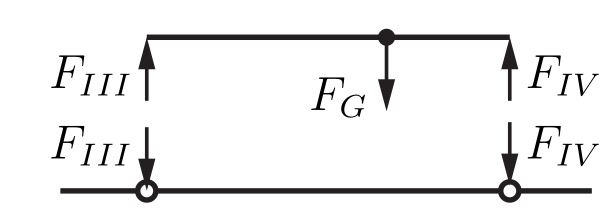
\includegraphics[width= 10cm]{tikz/28_09_2018_1a}
\end{figure}
\newline
Die Gleichgewichtsbedingungen lauten
\begin{align*}
	\textbf{e}_y &: F_{III} - F_G + F_{IV} = 0 \\
	\textbf{e}_z &: -F_{III}k + F_{IV}l = 0
\end{align*}
Aus diesen beiden Gleichungen folgen schließlich die beiden Kräfte 
\begin{align*}
	F_{III} &= \frac{l}{k + l}F_G \\
	F_{IV} &= \frac{k}{k + l}F_G
\end{align*}
b) \\ \\
Die Gleichgewichtsbedingungen mit den beiden Lagern lauten
\begin{align*}
	\textbf{e}_x &: F_{A,x} = 0\\
	\textbf{e}_y &: F_{A,y} - F_{III} - F_{IV} + F_B = 0\\
	\textbf{e}_z &: -F_{III}2a  - F_{IV}3a + F_B4a = 0
\end{align*}
Aus diesen Gleichungen folgen die Lagerkräfte
\begin{align*}
	F_{A,x} &= 0 \\
	F_{A,y} &= \frac{2l + k}{4a}F_G \\
	F_B &= \frac{2l + 3k}{4a}F_G
\end{align*}
c)\\ \\
Mit der Momentengleichung
\[
	\textbf{e}_z : -F_{A,y}2a + F_6h = 0 
\]
im Knoten III folgt die Stabkraft
\[
	F_6 = \frac{2l + k}{2h}F_G
\]
Aus diesem Ergebnis ergibt sich das der Stab 6 ein Zugstab ist. \\ \\
d)\\ \\
Durch einfaches Überlegen ergibt sich das Stab 1 ein Druck- und Stab 2 ein Zugstab ist. Die bestimmte Höhe beträgt
\[
	h = \sqrt{3}a
\]
e) \\ \\
Aus 
\begin{align*}
	\textbf{e}_x &: F_1 - F_4 = 0\\
	\textbf{e}_y &: F_3 = 0
\end{align*}
ist ersichtlich, dass auf den Stab 3 keine Kraft ausgeübt wird. \\ \\
	\textbf{Beispiel 2}\\ \\
a) \\ \\
Der Wärmestrom der über den Boden strömt lautet
\[
	\dot{Q}_b = 2RL\alpha_b(T_H - T_B)
\]
b) \\ \\
Der Wärmestrom der über das Dach abfließt kann mit der Energiebilanz bestimmt werden. Dieser lautet somit
\[
	\dot{Q}_r = \dot{Q}_O - \dot{Q}_b
\]
c)\\ \\
Die Isolierschicht muss die Dicke
\[
	d = R\left(\exp\left(\frac{\lambda\pi L(T_H - T_A)}{\dot{Q}_0 - \dot{Q}_b} - \frac{\lambda}{R\alpha_i}\right) - 1\right)
\]
betragen, damit sich die Temperatur $T_H$ stationär im Habitat einstellt.\\ \\
d)\\ \\
Der geforderte Sichtfaktor wird mit der Cross-String-Methode ermittelt und lautet 
\[
	F_{BD} = \frac{2\sqrt{H^2 + 4R^2} - 2H}{4R} = \frac{\sqrt{H^2 + 4R^2} - H}{2R}
\]
	\newpage
\noindent
\textbf{Beispiel 1}\\ \\
a)\\ \\
Dieses System besitzt genau einen Freiheitsgrad und der lautet
\[
	\textbf{q}^T = \begin{bmatrix}
		\alpha
	\end{bmatrix}
\]
b)\\ \\
Der Abstand $s$ lautet
\[
	s = \sqrt{(R - r)^2 - \left(\frac{l}{2}\right)^2}
\]
und der Winkel $\gamma$ lautet
\[
	\gamma = \arcsin\left(\frac{l}{2(R - r)}\right)
\]
c)\\ \\
Der Ortsvektoren zum Schwerpunkt lautet für die Grundplatte
\[
	\textbf{r}_G = \begin{bmatrix}
		s\cos(\alpha) \\
		s\sin(\alpha)
	\end{bmatrix}
\]
für die Vorderrolle
\[
	\textbf{r}_{RV} = \begin{bmatrix}
		(R - r)\cos(\alpha - \gamma) \\
		(R - r)\sin(\alpha -  \gamma)
	\end{bmatrix}
\]
und für die Hinterrolle
\[
	\textbf{r}_{RH} = \begin{bmatrix}
		(R - r)\cos(\alpha + \gamma) \\
		(R - r)\sin(\alpha + \gamma)
	\end{bmatrix}
\]
d) \\ \\
Die geforderten Werte lauten für die Grundplatte
\begin{align*}
	\textbf{v}_G &= \begin{bmatrix}
		-s\sin(\alpha)\dot{\alpha} \\
		s\cos(\alpha)\dot{\alpha}
	\end{bmatrix}
	\\
	||\textbf{v}_G|| &= s\dot{\alpha} \\
	\omega_G &= \dot{\alpha}
\end{align*}
für die Vorderrolle
\begin{align*}
	\textbf{v}_{RV} &= \begin{bmatrix}
		-(R - r)\sin(\alpha - \gamma)\dot{\alpha} \\
		(R - r)\cos(\alpha - \gamma)\dot{\alpha}	
	\end{bmatrix}
	\\
	||\textbf{v}_{RV}|| &= (R - r)\dot{\alpha} \\
	\omega_{RV} &= \frac{r - R}{r}\dot{\alpha}
\end{align*}
und für die Hinterrolle
\begin{align*}
	\textbf{v}_{RH} &= \begin{bmatrix}
	-(R - r)\sin(\alpha + \gamma)\dot{\alpha} \\
	(R - r)\cos(\alpha + \gamma)\dot{\alpha}	
	\end{bmatrix}
	\\
	||\textbf{v}_{RH}|| &= (R - r)\dot{\alpha} \\
	\omega_{RH} &= \frac{r - R}{r}\dot{\alpha}
\end{align*}
e)\\ \\
Die kinetische Energie dieses Systems setzt sich aus der translatorischen und rotatorischen Teilenergie zusammen. Diese lauten
\begin{align*}
	T_t &= \frac{1}{2}||\textbf{v}_G||^2m_G + \frac{1}{2}||\textbf{v}_{RV}||^2m_R +\frac{1}{2}||\textbf{v}_{RH}||^2m_R \\
	&= \frac{1}{2}m_gs^2\dot{\alpha}^2 + \frac{1}{2}m_R(R - r)^2\dot{\alpha}^2 + \frac{1}{2}m_R(R - r)^2\dot{\alpha}^2 \\ \\
	T_r &= \frac{1}{2}\omega_G^2I_G + \frac{1}{2}\omega_{RV}I_R + \frac{1}{2}\omega_{RH}I_R
\end{align*}
Damit ergibt sich für die gesamte kinetische Energie des Systems
\begin{align*}
	T &= T_t + T_r \\
	  &= \frac{1}{2}m_gs^2\dot{\alpha}^2 + \frac{1}{2}m_R(R - r)^2\dot{\alpha}^2 + \frac{1}{2}m_R(R - r)^2\dot{\alpha}^2 + \frac{1}{2}\omega_G^2I_G + \frac{1}{2}\omega_{RV}I_R + \frac{1}{2}\omega_{RH}I_R
\end{align*}
f)\\ \\
Die potentiellen Teilenergien lauten
\begin{align*}
	V_G &= -m_Gg\sin(\alpha) \\
	V_{RV} &= -m_Rg(R - r)\sin(\alpha -  \gamma) \\
	V_{RH} &= -m_Rg(R - r)\sin(\alpha +  \gamma)
\end{align*}
Damit ergibt sich für die gesamte potentielle Energie des Systems
\begin{align*}
	V &= V_G + V_{RV} + V_{RH} \\
	  &= -m_Gg\sin(\alpha) - m_Rg(R - r)\sin(\alpha -  \gamma) - m_Rg(R - r)\sin(\alpha +  \gamma)
\end{align*}
g)\\ \\
Der Vektor der externen Kraft lautet
\[
	\textbf{F}_R = F_R\begin{bmatrix}
		\sin(\alpha) \\
		-\cos(\alpha)
	\end{bmatrix}
\]
Der Ortsvektor zum Angriffspunkt dieser Kraft lautet wiederum
\[
	\textbf{r}_F = \begin{bmatrix}
		s\cos(\alpha) \\
		s\sin(\alpha)
	\end{bmatrix}
\]
Damit lautet die generalisierte Kraft
\[
	\tau_{F_R} = \left(\frac{\partial \textbf{r}_F}{\partial \textbf{q}}\right)^T\textbf{F}_R = -sF_R
\]
h)\\ \\
Um den Euler-Lagrange-Formalismus durchzuführen benötigt man erstmal die Lagrange-Funktion. Diese lautet
\begin{align*}
	L &= T - V \\
	  &= \frac{1}{2}m_gs^2\dot{\alpha}^2 + \frac{1}{2}m_R(R - r)^2\dot{\alpha}^2 + \frac{1}{2}m_R(R - r)^2\dot{\alpha}^2 + \frac{1}{2}\omega_G^2I_G + \frac{1}{2}\omega_{RV}I_R + \frac{1}{2}\omega_{RH}I_R \\
	  &+ m_Gg\sin(\alpha) + m_Rg(R - r)\sin(\alpha -  \gamma) + m_Rg(R - r)\sin(\alpha +  \gamma)
\end{align*}
Die notwendigen Ableitungen lauten
\begin{align*}
	\frac{\partial L}{\partial \alpha} &= m_Gg\cos(\alpha) + m_Rg(R - r)\cos(\alpha - \gamma) + m_Rg(R - r)\cos(\alpha + \gamma) \\
	\frac{\partial L}{\partial \dot{\alpha}} &= m_Gs^2\dot{\alpha} + m_R(R - r)\dot{\alpha} + m_R(R - r)\dot{\alpha} + \dot{\alpha}I_G  + 2\left(\frac{r - R}{r}\right)^2\dot{\alpha}I_R \\
	\frac{\text{d}}{\text{d}t}\frac{\partial L}{\partial \dot{\alpha}} &= \ddot{\alpha}\left(m_Gs^2 +  m_R(R - r) + m_R(R - r) + 2\left(\frac{r - R}{r}\right)^2I_R\right)
\end{align*}
Somit lautet die Euler-Lagrange-Gleichung
\begin{align*}
	\ddot{\alpha}&\left(m_Gs^2 +  m_R(R - r) + m_R(R - r) + 2\left(\frac{r - R}{r}\right)^2I_R\right) \\
	&-m_Gg\cos(\alpha) - m_Rg(R - r)\cos(\alpha - \gamma) - m_Rg(R - r)\cos(\alpha + \gamma) = -sF_R
\end{align*}
Durch Umformen erhält man die Bewegungsgleichung
\[
	\ddot{\alpha} = \frac{g(m_Gs\cos(\alpha) + m_R(R - r)(\cos(\alpha - \gamma) + \cos(\alpha + \gamma)))}{2\left(\frac{1}{2}m_Gs^2 + m_R(R - r)^2 + \frac{1}{2}I_G + I_R\left(\frac{r - R}{r}\right)^2\right)}
\]
	\textbf{Beispiel 4}\\ \\
a)\\ \\
Die Differentialgleichung für das Heißgetränk lautet
\begin{align*}
	\rho c_p dh \frac{\partial T_H(t)}{\partial t} &= -(\dot{q} + \dot{q}_{HU}) \\
	\frac{\partial T_H(t)}{\partial t} &= \left(\frac{4k_bh + \alpha_{HU}d}{\rho c_p dh}\right)(T_h(t) - T_U)
\end{align*}
b)\\ \\
Die Lösung dieser Differentialgleichung lautet
\[
	T_H(t) = T_U + (T_0 - T_U)e^{-\left(\frac{4k_bh + \alpha_{HU}d}{\rho c_p dh}\right)t}
\]
c)\\ \\
Die spezifische Wärmekapazität des Gemisches lautet
\[
	c_{p,G} = \frac{c_{p,M}\beta + c_{p,H}}{1 - \beta}
\]
d) \\ \\
Die Temperatur des Gemisches lautet
\[
	T_G = \frac{c_{p,M}\beta T_M + c_{p,H}T_H}{c_{p,M} + c_{p,H}}
\]
e)\\ \\
i)\\
Durch Einsetzen der Bedingungen in die Lösung der Differentialgleichung folgt für $t_1$
\[
	t_1 = -\frac{\rho(c_{p,M}\beta + c_{p,H})dh}{4k_Bh + \alpha_{HU}d}\ln\left(\frac{(c_{p,M}\beta + c_{p,H})T_T - c_{p,M}\beta T_M + c_{p,H}T_U}{c_{p,H}(T_0 - T_U)}\right)
\]
ii)\\
Durch Einsetzen der Bedingungen in die Lösung der Differentialgleichung folgt für $t_2$
\[
	t_2 = -\frac{\rho c_{p,H}dh}{4k_Bh + \alpha_{HU}d}\ln\left(\frac{(c_{p,M}\beta + c_{p,H})T_T - c_{p,M}\beta T_M + c_{p,H}T_U}{c_{p,H}(T_0 - T_U)}\right)
\]
f)\\ \\
Durch Einsetzen der Bedingungen aus der Angabe ergibt sich für das Mischverhältnis $\beta > 0$.
	
	
	\subsection{30.11.2018}
	\subsection{01.02.2019}
	
	\newpage
	\subsection{15.03.2019} %schreibt Andi fertig, falls ich dann nicht auch schon dort sein sollte
	%\documentclass{article}
%\usepackage{tikz}
%\usepackage{amsmath}
%\begin{document}
\noindent
\textbf{Beispiel 1} \\ \\
a) 
	\begin{figure}[h]
		\centering
		\usetikzlibrary{arrows}
\tikzset{
pil/.style={
	->,thick,
	shorten<=2pt,
	shorten>=2pt,}
}
\begin{tikzpicture}[scale=0.75]
\draw (-5,0)--(5,0); %Grundfläche
\draw(-4.5,-0.075)--(-4.25,-0.75)--(-4,-0.075)--(-4.5,-0.075); %Gleitlager
\draw [fill=white]  (-4.25,-0.75) circle [radius=5pt];
\draw(4.5,0)--(4.25,-0.75)--(4,0); %Festlager
\draw [fill=white]  (4.25,-0.75) circle [radius=5pt];

\draw [fill=white] (-3,0) rectangle (3,3);
%Kräfte
\draw [->](0,2)--(0,1);
\draw (0.25,1.5) node {\(f_g\)};
\draw [<-](-4.25,-1.25) -- (-4.25,-2.25);
\draw  (-3.75,-2) node {\(f_{A,y}\)};
\draw [<-](4.25,-1.25) -- (4.25,-2.25);
\draw  (4.8,-1.85) node {\(f_{B,y}\)};
\draw [<-](4.75,-0.75) -- (5.75,-0.75);
\draw  (5.25,-0.5) node {\(f_{B,x}\)};
%\draw [fill=blue] (0,0) arc [start angle=90,end angle=300, radius=10pt];
%\draw  [fill=blue] (0,0) -- (2,0.5);



\end{tikzpicture}
	\end{figure} \\
%\noindent
Um die Kräfte in den Lagern zu bestimmten, stellen wir zuerst das Kräftegleichgewicht und die Momenten Gleichung im Punkt B auf. 
\begin{align*}\label{key}
x&: 0=f_{B,x} \\
y&: 0 = f_A + f_{B,y} -f_g\\
M_B&:0=b f_g-2L \cos(\alpha)  
\end{align*}

\noindent
Formt man nun die Momenten Gleichung nach \(f_A\) um folgt: 
\begin{align*}
f_A = \frac{b f_g}{2L \cos(\alpha)} \qquad f_{B_x}=0 \qquad f_{B,y} = \left(1-\frac{b}{2L \cos(\alpha)}\right) f_g
\end{align*}
\begin{figure}[h]
	\centering
	\begin{tikzpicture}[scale=0.5]

\node (v1) at (-2.5,-2.5) {};
\node (v2) at (2.5,2.5) {};
\node (v3) at (0,0) {};
\node (v4) at (-2.5,2.5) {};
\node (v5) at (2.5,-2.5) {};
\draw  (v1) circle (0.2);
\draw  (v2) circle (0.2);
\draw  (v3) circle (0.2);
\draw  (v4) circle (0.2);
\draw  (v5) circle (0.2);
\draw (-2.9,-2.2) -- (2.1,2.8);
\draw (-2.2,-2.9) -- (2.9,2.2);
\draw (-2.117,-2.8214) arc (-40.0022:-230:0.5);
\draw (2.117,2.8214) arc (139.9978:-40:0.5);
\draw (2,2.7) -- (2.2,2.9);
\draw[black!50] (-1.8,-2.5) -- (1.5,-2.5);

\draw (-0.6,-2.5) arc (0:19:3.1);
\draw  (-1,-2.1) node {\(\alpha\)};
\draw (-2.8,2.1) -- (2.1,-2.8);
\draw (-2.1,2.8) -- (2.9,-2.2);
\draw (2.117,-2.8214) arc (-139.9978:40:0.5);
\draw (-2.75,2.067) arc (-120.0007:-325:0.5);
\draw [->](0,-0.3) -- (0,-1.4) ;
\draw (1.2,-1.4) node {\(m_2 g\)};
\draw[<-] (2.5,-3.2) -- (2.5,-4.1);
\draw (3.5,-3.6) node {\(f_{E,y}\)};
\draw [<-](-2.5,-3.2) -- (-2.5,-4);
\draw (-1.5,-3.6) node {\(f_{D_y}\)};
\draw[<-] (2.5,3.2) -- (2.5,4.1);
\draw (3.5,3.6) node {\(f_{B,y}\)};
\draw [<-](-2.5,3.2) -- (-2.5,4);
\draw (-1.5,3.6) node {\(f_{A_y}\)};

\end{tikzpicture}
\end{figure}
b) \\
%\noindent
Um die Kräfte in den Punkten D und E zu bestimmen, stellen wir das Kräftegleichgewicht in den Trägern auf, daraus folgt: 
\begin{align*}
 f_{D,y} = m2 g + f_{B,y}\qquad	f_{E,y} = m_2 g + f_A 
\end{align*}

\begin{figure}[h]
	\centering
	\begin{tikzpicture}[scale=0.5]

\node (v1) at (-2.5,-2.5) {};
\node (v2) at (2.5,2.5) {};
\node (v3) at (0,0) {};
%\node (v4) at (-2.5,2.5) {};
%\node (v5) at (2.5,-2.5) {};
\draw  (v1) circle (0.2);
\draw  (v2) circle (0.2);
\draw  (v3) circle (0.2);
%\draw  (v4) circle (0.2);
%\draw  (v5) circle (0.2);
\draw (-2.9,-2.2) -- (2.1,2.8);
\draw (-2.2,-2.9) -- (2.9,2.2);
\draw (-2.117,-2.8214) arc (-40.0022:-230:0.5);
\draw (2.117,2.8214) arc (139.9978:-40:0.5);
\draw (2,2.7) -- (2.2,2.9);
\draw[black!50] (-1.8,-2.5) -- (1.5,-2.5);

\draw (-0.6,-2.5) arc (0:19:3.1);
\draw  (-1,-2.1) node {\(\alpha\)};
% \draw (-2.8,2.1) -- (2.1,-2.8);
% \draw (-2.1,2.8) -- (2.9,-2.2);
% \draw (2.117,-2.8214) arc (-139.9978:40:0.5);
% \draw (-2.75,2.067) arc (-120.0007:-325:0.5);
\draw [->](0,-0.3) -- (0,-1.4) ;
\draw (0.8,-1.0) node {\(m_2 g\)};
% \draw[<-] (2.5,-3.2) -- (2.5,-4.1);
% \draw (3,-3.6) node {\(f_{D,y}\)};
\draw [<-](-2.5,-3.2) -- (-2.5,-4);
\draw (-1.5,-3.6) node {\(f_{D_y}\)};
\draw[<-] (2.5,3.2) -- (2.5,4.1);
\draw (3.5,3.6) node {\(f_{B,y}\)};
% \draw [<-](-2.5,3.2) -- (-2.5,4);
%\draw (-2.0,3.6) node {\(f_{A_y}\)};



\draw [<-](-3.3,-2.5) -- (-4.2,-2.5);
\draw (-3.7,-3.2) node {\(f_{D,x}\)};
\draw [<-](3.3,2.5) -- (4.2,2.5);
\draw (3.7,1.7) node {\(f_{B,x}\)};
\end{tikzpicture}
\end{figure}
\noindent
c)\\  \\ %\noindent
Um die Kräfte in den Lagern D und E in horizontaler (x-Richtung) zu bestimmen schneiden wir die Hubstangen getrennt voneinander frei und stellen die Kraftgleichungen und die Momenten Gleichung auf. 

\begin{align*}
	x&:  0 = f_{E,x} - f_{D,x}\\
	y&:  \text{wurde bereits bestimmt} \\ 
	M_D&: 0 = m_2 g \cos(\alpha) +f_{B,x} \sin(\alpha) + f_{B,y} \cos(\alpha)
\end{align*}
Aus der Momenten Gleichung  folgt: 
\begin{align*}
	f_{B,x} = \frac{m_2 g- f_{B,y}}{\tan{\alpha}} =f_{E,x} \qquad  F(\alpha) = f_{D,x} = -f_{E,x}
\end{align*}
\noindent 
d) \\ \\ 	
	Um die Haftbedingung zu berechnen formt man \(F(\alpha) = \mu_H f_{D,y}\) um und setzt für \(\alpha=\frac{\pi}{4}\) ein: 
	
	\begin{align*}
		\mu_H \geq \frac{F(\alpha)}{f_{D,y}} = \frac{m_1+m_2}{m_2+\frac{m_1 b}{\sqrt2L}}
	\end{align*}
	
%\end{document}	
	\newpage
\noindent
\textbf{Beispiel 2} \\ \\
a) \\ \\
%\noindent
Die Oberfläche des Öl's strahlt nicht auf sich selbst, deshalb lautet der Sichtfaktor Matrixeintrag \(F_{OO} = 0\), aus der Summationsregel folgt \(F_{OH} = 1 - F_{OO} = 1\). Aus dem Reziprozitätsgesetz folgt \(F_{HO}=\frac{A_O}{A_H}F_{OH} \). Der Letzte Eintrag lautet wegen der Summationsregel \(F_{HH}=1-\frac{A_O}{A_H}\)

\[\textbf{F}=\left[\begin{matrix}
0 & 1 \\ \frac{A_O}{A_H} & 1 -\frac{A_O}{A_H} \end{matrix}\right]\]

\begin{tiny}
%\hspace{100px}	
\( \hspace{-75pt}\dot{\textbf{q}}=  \left[ \begin {array}{c} \sigma\, \left(  \left( {\frac {\varepsilon_
		{H}\,A_{H}-\varepsilon_{H}\,A_{O}+A_{O}}{-A_{O}\,\varepsilon_{H}\,
		\varepsilon_{O}+\varepsilon_{H}\,A_{H}+A_{O}\,\varepsilon_{O}}}+{
	\frac { \left( -1+\varepsilon_{H} \right) A_{O}}{-A_{O}\,\varepsilon_{
			H}\,\varepsilon_{O}+\varepsilon_{H}\,A_{H}+A_{O}\,\varepsilon_{O}}}
\right) \varepsilon_{O}\,{{\it TO}}^{4}+ \left( -{\frac { \left( -1+
		\varepsilon_{O} \right) A_{H}}{-A_{O}\,\varepsilon_{H}\,\varepsilon_{O
		}+\varepsilon_{H}\,A_{H}+A_{O}\,\varepsilon_{O}}}-{\frac {A_{H}}{-A_{O
		}\,\varepsilon_{H}\,\varepsilon_{O}+\varepsilon_{H}\,A_{H}+A_{O}\,
		\varepsilon_{O}}} \right) \varepsilon_{H}\,{{\it TH}}^{4} \right) 
\\ \noalign{\medskip}\sigma\, \left(  \left( -{\frac {A_{O}\, \left( 
		\varepsilon_{H}\,A_{H}-\varepsilon_{H}\,A_{O}+A_{O} \right) }{A_{H}\,
		\left( -A_{O}\,\varepsilon_{H}\,\varepsilon_{O}+\varepsilon_{H}\,A_{H
		}+A_{O}\,\varepsilon_{O} \right) }}-{\frac {{A_{O}}^{2} \left( -1+
		\varepsilon_{H} \right) }{A_{H}\, \left( -A_{O}\,\varepsilon_{H}\,
		\varepsilon_{O}+\varepsilon_{H}\,A_{H}+A_{O}\,\varepsilon_{O} \right) 
}} \right) \varepsilon_{O}\,{{\it TO}}^{4}+ \left( {\frac {A_{O}\,
		\left( -1+\varepsilon_{O} \right) }{-A_{O}\,\varepsilon_{H}\,
		\varepsilon_{O}+\varepsilon_{H}\,A_{H}+A_{O}\,\varepsilon_{O}}}+{
	\frac {A_{O}}{-A_{O}\,\varepsilon_{H}\,\varepsilon_{O}+\varepsilon_{H}
		\,A_{H}+A_{O}\,\varepsilon_{O}}} \right) \varepsilon_{H}\,{{\it TH}}^{
	4} \right) \end {array} \right] 
\)
\end{tiny}
\\ \newline
\bigskip
\noindent
Um diesen Vektor zu ermitteln, wird einfach der Formalismus der Nettowärmestromdichte genutzt.
Der Vektor \(\dot{\textbf{q}}\) besteht aus den Einträgen \(\dot{q}_O\) und \(\dot{q}_H\), wir benötigen aber nur den ersten Eintrag, weil \(\dot{Q}_{rad} = A_O \dot{q}_O\) lautet.
\bigskip \\
b) \\
\\
Um die stationäre thermische Energiebilanz zu bestimmen müssen alle Wärmeströme die ein- oder austreten addiert werden. 

\[\dot{m}_{LM} c_{p,LM} (T_\infty-T_L)+0.2\dot{m}_{LM} c_{p,O}-A_O \alpha_{OL}(T_O-T_\infty)-\dot{Q}_{rad}+P_{el}\eta=0\]
\bigskip 

\noindent c)  \\ 
\\ 
Die Temperatur \(T_O\) lautet nun \(\overline{T}_O\) und wird in die Lösung von b eingesetzt. Danach muss die Gleichung nach \(P_{el}\) umgeformt werden. Daraus ergibt sich. 

\[P_{el}=\frac{1}{\eta}\left(-\dot{m}_{LM} c_{p,LM} (T_\infty-T_L)-0.2\dot{m}_{LM} c_{p,O}-A_O \alpha_{OL}(T_O-T_\infty)+\dot{Q}_{rad}\right)\]

\bigskip 

\noindent d)  \\ 
\\
Die Anfangsbedienung der Differentialgleichung lautet \(T_O(t=0)=\overline{T}_O\) und die Differentialgleichung erhält man indem man die Fouriersche Wärmeleitgleichung nach dem Volumen integriert. Zu beachten ist das auf der rechten Seite alle ein- und ausfließenden Wärmeströme stehen: 
\[
\int \rho c_{p,O} \frac{\partial T_O}{\partial t} dV = \int -\alpha_{O,L}(T_O-T_\infty) - \dot{q}_{rad}\, dA
\]
\[
m_O\,c_{p,O} \frac{\partial T_O}{\partial t} = A_O \alpha_{O,L} (T_O-T_\infty) - \dot{Q}_{rad}
\]
\[
T_0(t=0)= \overline{T}_O
\]
	
	\newpage	
	\subsection{17.05.2019}
	\textbf{Beispiel 3} \\ \\
	a) \\ \\
	Der Vektor vom Ursprung zum Schwerpunkt des Rades kann direkt aus Angabe abgelesen werden und lautet deshalb:
	\begin{align*}
		\textbf{r}_r = \left[ \begin{matrix}
			p\cos\alpha - r\sin\alpha \\
			p\sin\alpha + r\cos\alpha
		\end{matrix}\right]
	\end{align*}
	Der translatorische Geschwindigkeitsvektor erhält man durch die Ableitung vom Ortsvektor nach den Freiheitsgraden.\\ \\
	Translatorischer Geschwindigkeitsvektor:
	\[
			\textbf{v}_r = \dot{\textbf{r}_r} = \left[\begin{matrix}
			\dot{p}\cos\alpha \\
			\dot{p}\sin\alpha
		\end{matrix}\right]
	\]
	Die rotatorische Geschwindigkeit lautet:
	\[ \omega_r = \frac{\dot{p}}{r}\]
	b)\\ \\
	Der Vektor zum Schwerpunkt des Stabes kann ebenfalls aus der Angabe abgelesen werden und lautet deshalb:
	\begin{align*}
		\textbf{r}_S = \left[\begin{matrix}
			p\cos\alpha - r\sin\alpha + l_s\sin\varphi \\
			p\sin\alpha + r\cos\alpha + l_s\cos\varphi
		\end{matrix}\right]
	\end{align*}
	Analog zu a) lautet der translatorische Geschwindigkeitsvektor:
	\[
		\textbf{v}_S = \dot{\textbf{r}_S} =\left[ \begin{matrix}
			\dot{p}\cos\alpha + l_s\cos\varphi\dot{\varphi} \\
			\dot{p}\sin\alpha - l_s\sin\varphi\dot{\varphi}
		\end{matrix}\right]
	\]
	\newpage
	\noindent
	c) \\ \\
	Als erstes wird die translatorische kinetische Energie des System wie folgt ermittelt:\\ \\
	Vereinfachungen:
	\begin{align*}
		\dot{\textbf{r}_r}^T\dot{\textbf{r}_r} &= \left[ \begin{matrix}
			\dot{p}\cos\alpha & \dot{p}\sin\alpha
		\end{matrix}\right]
		\left[\begin{matrix}
			\dot{p}\cos\alpha \\
			\dot{p}\sin\alpha
		\end{matrix}\right] \\
		&= \dot{p}^2\cos^2\alpha + \dot{p}^2\sin^2\alpha \\
		&= \dot{p}^2\underbrace{\left( \cos^2\alpha + \sin^2\alpha\right)}_{=1} \\
		&= \dot{p}^2 
	\end{align*}
	\begin{align*}
		\dot{\textbf{r}_S}^T\dot{\textbf{r}_S} &= \left[\begin{matrix}
		\dot{p}\cos\alpha + l_s\cos\varphi\dot{\varphi} & \dot{p}\sin\alpha - l_s\sin\varphi\dot{\varphi}
		\end{matrix}\right] \left[\begin{matrix}
		\dot{p}\cos\alpha + l_s\cos\varphi\dot{\varphi} \\
		\dot{p}\sin\alpha - l_s\sin\varphi\dot{\varphi}
		\end{matrix}\right] \\
		&=\left(\dot{p}\cos\alpha + l_s\cos\varphi\dot{\varphi}\right)^2 + \left(\dot{p}\sin\alpha + l_s\sin\varphi\dot{\varphi}\right)^2 \\
		&=\dot{p}^2\cos^2\alpha + 2l_s\dot{p}\dot{\varphi}\cos\alpha\cos\varphi + l_s^2\dot{\varphi}^2\cos^2\varphi + \dot{p}^2\sin^2\alpha - 2l_s\dot{p}\dot{\varphi}\sin\alpha\sin\varphi + l_s^2\sin^2\varphi\dot{\varphi}^2 \\
		&=\dot{p}^2\underbrace{\left(\sin^2\alpha + \cos^2\alpha\right)}_{=1} + 2l_s\dot{p}\dot{\varphi}\underbrace{\left(\cos\varphi\cos\alpha - \sin\varphi\sin\alpha\right)}_{\cos\left(\varphi + \alpha\right)} + l_s^2\dot{\varphi}^2\underbrace{\left(\sin^2\varphi + \cos^2\varphi\right)}_{=1} \\
		&= \dot{p}^2 + 2l_s\dot{p}\dot{\varphi}\cos\left(\varphi + \alpha\right) + l_s^2\dot{\varphi}^2
	\end{align*}
	Nun kann man schließlich die translatorische kinetischen Energie des Rades und des Stabes bestimmen.
	\begin{align*}
		T_{trans,r} &=  \frac{1}{2}m_r\dot{p}^2\\
		T_{trans,s} &=  \frac{1}{2}m_s\left(\dot{p}^2 + l_s^2\dot{\varphi}^2 + 2l_s\dot{p}\dot {\varphi}\cos\left(\varphi + \alpha\right)\right)
	\end{align*}
	Die kinetische Energie besitzt jedoch auch einen rotatorischen Anteil. Dieser lautet für die beiden Teilsysteme:
	\begin{align*}
		T_{rot,r} &= \frac{1}{2} \Theta_r \frac{\dot{p}^2}{r^2} \\
		T_{rot,s} &= \frac{1}{2} \Theta_s \dot{\varphi}^2
	\end{align*}
	Da wir nun sämtliche Teilenergien ermittelt haben, beträgt die gesamte kinetische Energie des vorliegenden Systems:
	\begin{align*}
		T &= T_{trans,r} + T_{rot,r} + T_{trans,s} + T_{rot,s}\\
		  &= \frac{1}{2}m_r\dot{p}^2 + \frac{1}{2} \Theta_r \frac{\dot{p}^2}{r^2} + \frac{1}{2}m_s\left(\dot{p}^2 + l_s^2\dot{\varphi}^2 + 2l_s\dot{p}\dot{\varphi}\cos\left(\varphi + \alpha\right)\right) + \frac{1}{2} \Theta_s \dot{\varphi}^2
	\end{align*}
	\newpage
	\noindent
	Als nächstes wird nun die gesamte potentielle Energie des gegebenen System ermittelt. Zuerst berechnet man wieder die Energien der Teilsysteme und addiert dieser zum Schluss wieder zusammen.
	\begin{align*}
		V_r &= m_rg\left(p\sin\alpha + r\cos\alpha\right) \\
		V_s &= m_sg\left(p\sin\alpha + r\cos\alpha + l_s\cos\varphi\right) \\
		V = V_r + V_s &= m_rg\left(p\sin\alpha + r\cos\alpha\right) + m_sg\left(p\sin\alpha + r\cos\alpha + l_s\cos\varphi\right)
	\end{align*}
	d)\\ \\
	Um den Vektor der generalisierten Kräfte zu bestimmen benötigt man zuerst den Richtungsvektor zu den Angriffspunkten der extern wirkenden Kräfte, hier $f_{ext}$. \\ \\
	Angriffspunkt der Kraft:
	\[
		\textbf{r}_f = \left[\begin{matrix}
			p\cos\alpha - r\sin\alpha + 2l_s\sin\varphi \\
			p\sin\alpha + r\cos\alpha + 2l_s\cos\varphi
		\end{matrix}\right]
	\]
	Weiters benötigt man auch den Vektor der externen Kräfte. \\ \\
	Kraftvektor:
	\[
		\textbf{f}_{ext}^T = f_{ext}\left[\begin{matrix}
			\cos\beta & \sin\beta
		\end{matrix}\right]
	\]
	Nun werden die partiellen Ableitung nach $\textbf{q}$ vom Angriffspunkt der Kraft gebildet:
	\begin{align*}
		\frac{\partial\textbf{r}_f}{\partial\varphi} = \left[\begin{matrix}
			2l_s\cos\varphi \\
			-2l_s\sin\varphi
		\end{matrix}\right] \qquad
		\frac{\partial\textbf{r}_f}{\partial p} = \left[\begin{matrix}
			\cos\alpha \\
			\sin\alpha
		\end{matrix}\right]
	\end{align*}
	Der Vektor der generalisierten Kräfte wird nun wie folgt ermittelt:
	\begin{align*}
		\textbf{f}_q = \textbf{f}_{ext}^T \frac{\partial \textbf{r}_f}{\partial \textbf{q}}
	\end{align*}
	generalisierte Kräfte:
	\begin{align*}
		f_{q,\varphi} &= f_{ext}\left[\begin{matrix}
		\cos\beta & \sin\beta
		\end{matrix}\right] \left[\begin{matrix}
		2l_s\cos\varphi \\
		-2l_s\sin\varphi
		\end{matrix}\right] \\
		&= f_{ext} \left(2l_s\cos\beta\cos\varphi - 2l_s\sin\beta\sin\varphi\right) \\
		&= f_{fext}2l_s \underbrace{\left(\cos\beta\cos\varphi - 2l_s\sin\beta\sin\varphi\right)}_{\cos\left(\beta + \varphi\right)} \\
		&= f_{ext}2l_s\cos\left(\beta + \varphi\right)
	\end{align*}
	\begin{align*}
		f_{q,p} &= f_{ext} \left[\begin{matrix}
		\cos\beta & \sin\beta
		\end{matrix}\right] \left[\begin{matrix}
			\cos\alpha \\
			\sin\alpha
		\end{matrix}\right] \\
		&= f_{ext} \underbrace{\left(\cos\beta\cos\alpha + \sin\beta\sin\alpha\right)}_{\cos\left(\beta - \alpha\right)} \\
		&= f_{ext} \cos\left(\beta - \alpha\right)
	\end{align*}
	gesamter Vektor:
	\[
		\textbf{f}_q = f_{ext} \left[\begin{matrix}
			2l_s\cos\left(\beta + \varphi\right) \\
			\cos\left(\beta - \alpha\right)
		\end{matrix}\right]
	\]
	\newpage
	\noindent
	e) \\ \\
	Zum Schluss sollen noch die Bewegungsgleichungen mithilfe des Euler-Lagrange-Formalismus bestimmt werden.
	\begin{align*}
		L &= T - V \\
		 &= \frac{1}{2}m_r\dot{p}^2 + \frac{1}{2} \Theta_r \frac{\dot{p}^2}{r^2} + \frac{1}{2}m_s\left(\dot{p}^2 + l_s^2\dot{\varphi}^2 + 2l_s\dot{p}\dot{\varphi}\cos\left(\varphi + \alpha\right)\right) + \frac{1}{2} \Theta_s \dot{\varphi}^2 \\
		 & - m_rg\left(p\sin\alpha + r\cos\alpha\right) - m_sg\left(p\sin\alpha + r\cos\alpha + l_s\cos\varphi\right)
	\end{align*}
	Bewegungsgleichungen:
	\begin{align*}
		\frac{d}{dt}\left(\frac{\partial L}{\partial \dot{\varphi}}\right) - \left(\frac{\partial L}{\partial \varphi}\right) &= 2l_sf_{ext}\cos\left(\beta + \varphi\right) \\
		\frac{d}{dt}\left(\frac{\partial L}{\partial \dot{p}}\right) - \left(\frac{\partial L}{\partial p}\right) &= f_{ext}\cos\left(\beta - \alpha\right)
	\end{align*}
	Zwischenschritte:
	\begin{align*}
		\frac{\partial L}{\partial \dot{\varphi}} &= m_s\left(l_s^2\dot{\varphi} + l_s\dot{p}\cos\left(\varphi + \alpha\right)\right) + \Theta_s \dot{\varphi} \\
		\frac{\partial L}{\partial \dot{p}} &= m_r\dot{p} + \frac{\Theta_r}{r^2}\dot{p} + m_s\left(\dot{p} + 2l_s\dot{\varphi}\cos\left(\varphi + \alpha\right)\right)
	\end{align*}
	auftretende Ableitungen:
	\begin{align*}
		\frac{\partial L}{\partial \varphi} &= -m_sl_s\sin\left(\varphi + \alpha\right)\dot{p}\dot{\varphi} + m_sgl_s\sin\varphi \\
		\frac{\partial L}{\partial p} &= -g\left(m_s + m_r\right)\sin\alpha \\
		\frac{d}{dt}\left(\frac{\partial L}{\partial \dot{\varphi}}\right) &= m_sl_s\cos\left(\varphi + \alpha\right)\ddot{p} + \left(m_sl_s^2 + \Theta_s\right)\ddot{\varphi} - m_sl_s\dot{p}\sin\left(\varphi + \alpha\right)\dot{\varphi} \\
		\frac{d}{dt}\left(\frac{\partial L}{\partial \dot{p}}\right) &= \left(m_r + \frac{\Theta_r}{r^2} + m_s\right)\ddot{p} + m_sl_s\left(\ddot{\varphi}\cos\left(\varphi + \alpha\right) - \dot{\varphi}\sin\left(\varphi + \alpha\right)\dot{\varphi} \right)
	\end{align*}
	
	\newpage
	\subsection{12.07.2019}
	\noindent
\textbf{Beispiel 1} \\ \\
a) \\ \\
Der Richtungsvektor vom Urspung zum Schwerpunkt der Masse $m$ lautet:
\[
	\textbf{p}_m = \left[ \begin {array}{c} r\cos \left( \alpha \right) +b
	\\ r\sin \left( \alpha \right) -h\end {array}
	\right]	
\]
Mithilfe diesen Vektor kann ebenfalls auch der Geschwindigkeitsvektor bestimmt werden, indem man den Richtungsvektor nach der Zeit ableitet.
\[
	\dot{\textbf{p}}_m =\left[ \begin {array}{c} -r \dot{\alpha}
	  \sin \left( \alpha 
	\right) + \dot{b} \\ 
	r \dot{\alpha} \cos \left( \alpha  \right) -
		\dot{h} \end {array} \right] 
\]
b) \\ \\
Um die kinetischen Energien zu berechnen, müssen zuerst einige Nebenrechnungen durchgeführt werden.\\
Nebenrechnungen:
\begin{align}
	\dot{\textbf{p}}_m^T \dot{\textbf{p}}_m &= \left[ \begin{matrix}
		-r\dot{\alpha}\sin \left( \alpha \right) + \dot{b} & r\dot{\alpha}\cos \left( \alpha \right) -\dot{h}
	\end{matrix}\right] \left[ \begin {array}{c} -r \dot{\alpha}
	\sin \left( \alpha 
	\right) + \dot{b} \\ 
	r \dot{\alpha} \cos \left( \alpha  \right) -
	\dot{h} \end {array} \right] \\
	&= r^2\dot{\alpha}^2\underbrace{\left(\cos \ \alpha  + \sin  \alpha\right)  }_{=1} -2r\dot{\alpha}\dot{b}\sin\alpha - 2r\dot{\alpha}\dot{h}\cos\alpha + \dot{b}^2 + \dot{h}^2 \\
	&= r^2\dot{\alpha}^2 -2r\dot{\alpha}\dot{b}\sin\alpha - 2r\dot{\alpha}\dot{h}\cos\alpha + \dot{b}^2 + \dot{h}^2 \\
	\varphi &= \arctan\left(\frac{h}{b}\right) \\
	\dot{\varphi} &= \frac{\dot{h}b - h\dot{b}}{b^2 + h^2}
\end{align}
kinetische Energie des Systems:
\begin{align*}
	T_{tm} &= \frac{1}{2}m\dot{\textbf{p}}_m^T \dot{\textbf{p}}_m = \frac{1}{2} m \left( r^2\dot{\alpha}^2 -2r\dot{\alpha}\dot{b}\sin\left(\alpha\right) - 2r\dot{\alpha}\dot{h}\cos\left(\alpha\right) + \dot{b}^2 + \dot{h}^2\right) \\
	T_{rm} &= \frac{1}{2} \Theta_m\dot{\varphi}^2 = \frac{1}{2} \Theta_m \left( \frac{\dot{h}b - h\dot{b}}{b^2 + h^2}\right)^2 \\
	T_{rr} &= \frac{1}{2}\Theta_r\dot{\alpha}^2 \\
	T &= T_{tm} + T_{rm} + T_{rr} \\
	  &= \frac{1}{2}m\dot{\textbf{p}}_m^T \dot{\textbf{p}}_m = \frac{1}{2} m \left( r^2\dot{\alpha}^2 -2r\dot{\alpha}\dot{b}\sin\left(\alpha\right) - 2r\dot{\alpha}\dot{h}\cos\left(\alpha\right) + \dot{b}^2 + \dot{h}^2\right) 
	  + \frac{1}{2} \Theta_m \left( \frac{\dot{h}b - h\dot{b}}{b^2 + h^2}\right)^2 + \frac{1}{2}\Theta_r\dot{\alpha}^2
\end{align*}
\newpage
\noindent
c) \\ \\
potentielle Energie des Systems:
\begin{align*}
	V_m &= mg\left(r\sin\alpha - h\right) \\
	V_c &= \frac{1}{2} c \left(\sqrt{b^2 + h^2} s_0\right)^2 \\
	V &= V_m + V_c = mg\left(r\sin\alpha - h\right) + \frac{1}{2} c \left(\sqrt{b^2 + h^2} s_0\right)^2
\end{align*}
d) \\ \\
Die viskose Reibkraft muss in der Form $f_r = \mu_V \Delta v$ beschrieben werden. In diesen Beispiel ist $\Delta v = \dot{\varphi}\textbf{r}$. \textbf{r} ist der Vektor vom Angriffspunkt der Feder zum Schwerpunkt der Masse.
\[
	\textbf{f}_V = \mu_V \underbrace{\frac{\dot{h}b - h\dot{b}}{b^2 + h^2}}_{\dot{\varphi}} \underbrace{\begin{bmatrix}
	b \\ -h
	\end{bmatrix}}_{\textbf{r}}
\]
partielle Ableitungen:
\[
	\frac{\partial \dot{\textbf{p}}_m}{\partial \alpha}  = \left[ \begin{matrix}
		-r\sin\alpha \\ r\cos\alpha
	\end{matrix}\right] \qquad \frac{\partial \dot{\textbf{p}}_m}{\partial b} = \left[ \begin{matrix}
	 1 \\ 0
	\end{matrix}\right] \qquad \frac{\partial \dot{\textbf{p}}_m}{\partial h} = \left[ \begin{matrix}
	0 \\ -1
	\end{matrix}\right]
\]
\noindent
generalisierte Kräfte:\\ \\
Multipliziert man die viskose Reibungskraft mit allen partiellen Ableitungen erhält man
\begin{align*}
	\textbf{f}_{q,v} &= \mu_V \frac{\dot{h}b - h\dot{b}}{b^2 + h^2} \left[ \begin{matrix}
		r\sin\alpha b + r\cos\alpha h \\
		-b \\
		-h
	\end{matrix}\right]
\end{align*}
Die andere externe Kraft ist
\[
	\textbf{f}_x = \left[ \begin{matrix}
		f_x \\
		0
	\end{matrix}\right]
\]
Multipliziert mit den partiellen Ableitungen erhält man
\[
	\textbf{f}_{q,x} = \left[ \begin{matrix}
		-f_x r \sin\alpha \\
		f_x \\
		0
	\end{matrix}\right]
\]
Der gesamte Vektor der generalisierten Kräfte beträgt
\[
	\textbf{f}_q = \mu_V \frac{\dot{h}b - h\dot{b}}{b^2 + h^2} \left[ \begin{matrix}
	r\sin\alpha b + r\cos\alpha h \\
	-b \\
	-h
	\end{matrix}\right] 
	+ 
	\left[ \begin{matrix}
	-f_x r \sin\alpha \\
	f_x \\
	0
	\end{matrix}\right]
\]
e) \\ \\
Verwendet man aus der Formelsammlung im Punkt generalisierte Kräfte die 2.te Formel und passt man diese an den stationären Fall an erhält man
\[
	\frac{\partial V}{\partial \textbf{q}} = \left[ \begin{matrix}
		mgr\cos\alpha\\
		\frac{c\left( \sqrt{b^2 + h^2} - s_0\right)}{\sqrt{b^2 + h^2}} b \\
		\frac{c\left( \sqrt{b^2 + h^2} - s_0\right)}{\sqrt{b^2 + h^2}} h - mg
	\end{matrix}\right]
	=
	\left[ \begin{matrix}
	-f_x r \sin\alpha \\
	f_x \\
	0
	\end{matrix}\right]
\]
Nun wird $s_0$ mit 0 angenommen und anschließend werden die generalisierten Koordinaten bestimmt. \\ \\
1.Koordinate:
\begin{align*}
	mgr\cos\alpha &= -f_xr\sin\alpha \\
	-\frac{\cos\alpha}{\sin\alpha} &= \frac{mg}{f_x}  \\
	-\tan\alpha &= \frac{mg}{f_x} \\
	\alpha &= -\arctan\left( \frac{mg}{f_x}\right)
\end{align*}
2.Koordinate:
\begin{align*}
	\frac{c\left(\cancel{\sqrt{b^2 + h^2}}\right)}{\cancel{\sqrt{b^2 + h^2}}} b &= f_x \\
	cb &= f_x \\
	b &= \frac{f_x}{c}
\end{align*}
3.Koordinate
\begin{align*}
	\frac{c\left(\cancel{\sqrt{b^2 + h^2}}\right)}{\cancel{\sqrt{b^2 + h^2}}} h -mg &= 0 \\
	ch - mg &= 0 \\
	h &= \frac{mg}{c}
\end{align*}
f) \\ \\
Die resultierende Reibkraft wird mithilfe der Formel 2.96 aus dem Vorlesungsskript berechnet und lautet hier:
\[
	\textbf{f}_F = -c_W A \frac{\rho}{2} |\dot{\textbf{p}}_m|\dot{\textbf{p}}_m
\]
\begin{align*}
	|\dot{\textbf{p}}_m| &= \sqrt{\left( -r \dot{\alpha}
		\sin \left( \alpha 
		\right) + \dot{b}\right)^2 
	+
	\left( 	r \dot{\alpha} \cos \left( \alpha  \right) -
	\dot{h}\right)^2} \\
	&= \sqrt{r^2\dot{\alpha}^2\sin^2\alpha -2r\dot{\alpha}\dot{b}\sin\alpha + \dot{b}^2 + r^2\dot{\alpha}^2\sin^2\alpha - 2r\dot{\alpha}\dot{h}\cos\alpha + \dot{h}^2} \\
	&= \sqrt{r^2\dot{\alpha}^2\underbrace{\left(\sin^2\alpha + \cos^2\alpha\right)}_{=1} - 2r\dot{\alpha}\dot{b}\sin\alpha - 2r\dot{\alpha}\dot{h}\sin\alpha + \dot{b}^2 + \dot{h}^2} \\
	&= \sqrt{r^2\dot{\alpha}^2 - 2r\dot{\alpha}\dot{b}\sin\alpha - 2r\dot{\alpha}\dot{h}\sin\alpha + \dot{b}^2 + \dot{h}^2}
\end{align*}
Multipliziert man nun $\textbf{f}_F$ mit den partiellen Ableitungen aus d) und vereinfacht man so weit wie möglich erhält man
\begin{align*}
	\textbf{f}_{q,F} &= -c_W A \frac{\rho}{2}|\dot{\textbf{p}}_m|
	\left[\begin{matrix}
		r\dot{\alpha}\underbrace{\left( \sin^2\alpha + \cos^2\alpha \right)}_{=1} - r\dot{b}\sin\alpha - r\dot{h}\cos\alpha \\
		-r\dot{\alpha}\sin \left( \alpha \right) + \dot{b} \\
		-r\dot{\alpha}\cos \left( \alpha \right) +\dot{h}
	\end{matrix}
	\right] \\
	&= -c_W A \frac{\rho}{2}|\dot{\textbf{p}}_m|
	\left[\begin{matrix}
	r\dot{\alpha} - r\dot{b}\sin\alpha - r\dot{h}\cos\alpha \\
	-r\dot{\alpha}\sin \left( \alpha \right) + \dot{b} \\
	-r\dot{\alpha}\cos \left( \alpha \right) +\dot{h}
	\end{matrix}
	\right]
\end{align*}
	\newpage
\noindent
\textbf{Beispiel 2} \\ \\
a) \\ \\
Da es sich hier um ein Problem mit Zylinderkoordinaten hält, verwendet man nun einfach die Wärmeleitgleichung für Zylinderkoordinaten aus Formelsammlung und adaptiert diese entsprechend der Angabe. \\
\newline
Wärmeleitgleichung:
\[
	0 = \lambda \left( \frac{1}{r} \frac{d}{dr}\left( \frac{d}{dr} T_i\left( r\right)\right)\right)
\]
Die 0 auf der linken Seite beruht darauf, das es sich hier um ein stationäres Problem handelt und die Terme für $\varphi$ und $z$ fallen ebenfalls weg. \\
\newline
Lösung der DGL:
\begin{align*}
	\lambda_i \left( \frac{1}{r} \frac{d}{dr}\left( r \frac{d}{dr} T_i\left( r\right)\right)\right) &= 0
	\\
	\frac{d}{dr}\left( r \frac{d}{dr} T_i\left( r\right)\right) &= 0
	\\
	\int \frac{d}{dr}\left( r \frac{d}{dr} T_i\left( r\right)\right) dr &= \int 0 dr
	\\
	r \frac{d}{dr} T_i\left( r\right) &= C_3
	\\
	\frac{d}{dr} T_i\left( r\right) &= \frac{C_3}{r}
	\\
	\int \frac{d}{dr} T_i\left( r\right) dr &= \int \frac{C_3}{r} dr
	\\
	T_i\left( r\right) &= C_3 ln\left(r \right) + C_4
\end{align*}
Randbedingungen:
\begin{align*}
	T_i\left(2R\right) &= C_3 ln\left( 2R\right) + C_4 = T_2 \\
	T_i\left(2R\right) &= C_3 ln\left( 3R\right) + C_4 = T_3
\end{align*}
Integrationskonstanten: \\
\newline
Ausgehend von dem Gleichungssystem der Randbedingung kann man die Integrationskonstanten sehr leicht bestimmen. Als ersten formt man die 2.te Gleichung auf $C_4$ um.
\begin{align*}
	T_3 &= C_3 ln\left( 3R\right) + C_4\\
	C_4 &= T_3 - C_3 ln\left( 3R\right)
\end{align*}
Dann wird in Gleichung 1 eingesetzt
\begin{align*}
	T_2 &= C_3 ln\left( 2R\right) + T_3 - C_3 ln\left( 3R\right) \\
	T_2 - T_3 &= C_3 \underbrace{\left( ln\left( 2R\right) - ln\left( 3R\right) \right)}_{ln\left( \frac{2}{3}\right)} \\
	C_3 &= \frac{T_2 - T_3}{ln\left( \frac{2}{3}\right)}
\end{align*}
Nun setzt man $C_3$ in $C_4$ ein
\begin{align*}
	C_4 &= T_3 -  \frac{T_2 - T_3}{ln\left( \frac{2}{3}\right)} ln\left( 3R\right) \\
	C_4 &= \frac{T_3 \left( ln\left( 2R\right) - ln\left( 3R\right) \right)}{ln\left( \frac{2}{3}\right)} - \frac{T_2 - T_3}{ln\left( \frac{2}{3}\right)} ln\left( 3R\right) \\
	C_4 &= \frac{T_3 ln\left( 2R \right) - T_2 ln\left( 3R\right)}{ln\left( \frac{2}{3}\right)}
\end{align*}
b) \\ \\	
Die Leistungsdichte $g$ wird wie folgt berechnet
\[
	g = \rho_e |\textbf{J}|^2 = \rho_e \left( \frac{I}{A}\right)^2
\]
mit
\[
	A = \left(4R^2 - R^2\right)\pi
\]
Dies ist die Fläche eine Hohlleiters. Setzt man nun diese in $g$ ein, erhält man
\[
	g = \rho_e \left( \frac{I}{\left(4R^2 - R^2\right)\pi}\right)^2
\]
c) \\ \\
DGL:
\begin{align*}
	\lambda_l \left( \frac{1}{r}\frac{d}{dr}\left( r\frac{d}{dr} T_l\left(r\right)\right)\right) + g = 0 \\
	\frac{d}{dr}\left( r\frac{d}{dr} T_l\left(r\right)\right) = -\frac{gr}{\lambda_l} \\
	\int \frac{d}{dr}\left( r\frac{d}{dr} T_l\left(r\right)\right) dr = \int -\frac{gr}{\lambda_l} dr \\
	 r\frac{d}{dr} T_l\left(r\right) = -\frac{gr^2}{2\lambda_l} + C_1 \\
	 \frac{d}{dr} T_l\left(r\right) = -\frac{gr}{2\lambda_l} + \frac{C_1}{r} \\
	 \int \frac{d}{dr} T_l\left(r\right) dr = \int -\frac{gr}{2\lambda_l} + \frac{C_1}{r} dr \\
	 T_l\left(r\right) = -\frac{gr^2}{4\lambda_l} + C_1\ln\left( r \right) + C_2
\end{align*}
Randbedingungen
\begin{align*}
	T_l\left(R\right) = -\frac{gR^2}{4\lambda_l} + C_1\ln\left(R\right) + C_2 = T_1 \\
	T_l\left(2R\right) = -\frac{g4R^2}{4\lambda_l} + C_1 \ln\left(2R\right) + C_2 = T_2
\end{align*}
\newpage
\noindent
Integrationskonstanten: \\ \\
Die beiden Konstanten werden wie in a) bestimmt.
\begin{align*}
	-\frac{gR^2}{4\lambda_l} + C_1\ln\left(R\right) + C_2 = T_1 \\
	C_2 = T_1 + \frac{gR^2}{4\lambda_l} - C_1\ln\left(R\right)
\end{align*}
Diese Gleichung wird nun in die andere eingesetzt und man erhält
\begin{align*}
	-\frac{g4R^2}{4\lambda_l} + C_1 \ln\left(2R\right) + T_1 + \frac{gR^2}{4\lambda_l} - C_1\ln\left(R\right) = T_2 \\
	\frac{g}{4\lambda_l}\left(R^2 - 4R^2\right) 
	+ T_1 - T_2 = C_1 \underbrace{\left( ln\ln\left(1\right) - \ln\left(2\right)\right)}_{\ln\left( \frac{1}{2}\right)} \\
	C_1 = \frac{\frac{g}{4\lambda_l}\left(R^2 - 4R^2\right) + T_1 - T_2}{\ln\left( \frac{1}{2}\right)}
\end{align*}
Rückeingesetzt erhält man
\begin{align*}
	C_2 &= T_1 + \frac{gR^2}{4\lambda_l} - \frac{\frac{g}{4\lambda_l}\left(R^2 - 4R^2\right) + T_1 - T_2}{\ln\left( \frac{1}{2}\right)}\ln\left(R\right) \\
	&= \frac{T_1\left(\ln\left(R\right) - \ln\left(2R\right)\right)}{ln\left(\frac{1}{2}\right)} + 
	\frac{\frac{gR^2}{4\lambda_l}\left(\ln\left(R\right) - \ln\left(2R\right)\right)}{\ln\left( \frac{1}{2}\right)} \\
	&- \frac{\frac{g}{4\lambda_l}\left(R^2\ln\left(R\right) - 4R^2\ln\left(R\right)\right) + T_1\ln\left(R\right) - T_2\ln\left(R\right)}{\ln\left( \frac{1}{2}\right)} \\
	&= \frac{\frac{g}{4\lambda_l}\left(4R^2\ln\left(R\right) - R^2\ln\left(2R\right)\right) + T_2\ln\left(R\right) - T_1\ln\left(2R\right)}{\ln\left(\frac{1}{2}\right)}
\end{align*}
d) \\ \\
Zur eindeutigen Bestimmung der Temperaturen \(T_1 , T_2 , T_3\) muss einfach nur die Gleichungen für die Wärmeübergänge aufstellen. Diese lauten für \\ \\
\(T_2:\)
\[
	\lambda_i\frac{d}{dr}T_i\left(r\right)|_{r = 2R} = \lambda_l \frac{d}{dr}T_l\left(r\right)|_{r = 2R}
\]
\(T_3:\)
\[
	\alpha_0\left(T_\infty - T_3\right) = \lambda_i\frac{d}{dr}T_i\left(r\right)|_{r = 3R}
\]
\(T_1:\)
\[
	\alpha_f\left(T_f - T_1\right) = -\lambda_l\frac{d}{dr}T_l\left(r\right)|_{r = R}
\]
\newpage
\noindent
e) \\ \\
1) Temperatur der Kühlflüssigkeit senken \\
2) Oberfläche der Isolierung vergrößern (z.B. durch Kühlrippen) \\
3) Wärmeleitfähigkeit der Isolierung vergrößern \\
\\
\textit{Hinweis}:\\
\textit{Die Lösung in diesen Punkt erhält man durch logisch denken.}

	\newpage
\noindent
\textbf{Beispiel 3} \\ \\
a)
\vspace{-15pt}
\usetikzlibrary{arrows}
\begin{figure}[h]
	\centering
\begin{tikzpicture}
\draw (-3.5,-1) -- (-3.5,-2) -- (-2,-2) -- (-2,-1) -- (-3.5,-1);
\draw (-2.75,-1) -- (-2.75,0.5);
\draw [-latex][red,very thick](-2.75,0.0232) -- (-2.75,1.0);
\draw[-latex][red,very thick](-2.75,-0.5) -- (-2.75, -1.5);
\draw (-2.3377,-1.4121) node {\( mg\)} ;
\draw (-2.228,0.8364) node {\( F_{s,1}\)};
\draw (-1.62,5.145) -- (-0.3,4.2);
\draw  (-2,4.5) circle (0.75);
\draw (-2.75,4.5) -- (-2.75,3.5);
\draw [-latex][red,very thick](-2.75,3.5) -- (-2.75,2.5);
\draw [-latex][red,very thick] (-3,4.5) -- (-2,4.5);
\draw [latex-][red,very thick]  (-2,4.5) -- (-2,6);
\draw [latex-][red,very thick]  (-2,4.5) -- (-2,3);
\draw [-latex][red,very thick](-1.8834,3.8167) arc (-67.5126:26.8608:0.8);
\node at (-2.2741,2.505) {\(F_{s,1}\)};
\node at (-1.6074,3.205) {\( F_{E,y}\)};
\node at (-3.249,4.755) {\(F_{E,x}\)};
\node at (-1.6074,5.755) {\(m_sg\)};
\node at (-1.6574,4.5217) {\( \tau\)};
\draw [-latex][red,very thick] (-0.3,4.2) --(0.5,3.6);
\node at (0.5,4) {\( F_{s,2}\)};
\draw [latex-][red,very thick](0.8,3.4) -- (1.5,2.9);
\draw (1.5,2.9) -- (2.2,2.4);
\node at (1.2,3.5) {\(F_{s,2}\)};
\node at (2.3,2.2) {Lager};
\end{tikzpicture}
\end{figure}
\\ 
Nun müssen die Gleichgewichtsbedingungen für diesen Schnitt bestimmt werden. Diese lauten hier
\begin{align*}
	&\sum M_E = 0: \\
	&\tau -F_{s,2}r + F_{s,1}r = 0 \\
	\\
	&\sum F_x = 0: \\
	&F_{E,x} + F_{s,2}\sin\left(\frac{\pi}{4}\right) = 0 \\
	&F_{E,x} + \frac{F_{s,}}{\sqrt{2}}= 0 \\
	\\
	&\sum F_y = 0:\\
	&F_{E,y} - F_{s,1} - F_{s,2}\sin\left(\frac{\pi}{4}\right) - m_sg = 0\\
	&F_{E,y} - F_{s,1} - \frac{F_{s,2}}{\sqrt{2}} - m_sg = 0
\end{align*}
\newpage
Nun werden die Kräfte im Punkt E und die Seilkräfte berechnet.
\begin{align*}
	&F_{s,1} = mg \\
	\\
	&\tau -F_{s,2}r + F_{s,1}r = 0 \\
	& F_{s,2} r = \tau + m g r \\
	& F_{s,2} = mg + \frac{\tau}{r} \\
	\\
	&F_{E,x} + \frac{F_{s,2}}{\sqrt{2}}= 0 \\
	&F_{E,x} + \frac{mg}{\sqrt{2}} + \frac{\tau}{r\sqrt{2}} = 0 \\
	&F_{E,x} = - \frac{mg}{\sqrt{2}} - \frac{\tau}{r\sqrt{2}} \\
	\\
	&F_{E,y} - F_{s,1} - \frac{F_{s,2}}{\sqrt{2}} - m_sg = 0 \\
	&F_{E,y} - mg - \frac{mg}{\sqrt{2}} - \frac{\tau}{r\sqrt{2}} - m_sg = 0 \\
	&F_{E,y} = mg \frac{\sqrt{2} + 1}{\sqrt{2}} + \frac{\tau}{r\sqrt{2}} + m_sg
\end{align*}
b)
\begin{figure}[h]
	\centering
\begin{tikzpicture}[scale = 1.5]
\draw (-0.5,0.5) -- (-2,1.5) -- (-0.5,1.5);
\draw [red,very thick][-latex](-3.5,1.5) -- (-2,1.5);
\node at (-3.5,1) {\( F_{B,x}\)};
\draw (-2,1.5) -- (-2,-2.5) -- (-0.5,-2.5);
\draw [red,very thick][-latex](-2,0) -- (-2,1.5); 
\node at (-1.5,0.5) {\(F_{B,y}\)};
\draw [red,very thick][-latex](-3.5,-2.5) -- (-2,-2.5);
\node at (-3.5,-2) {\(F_A\)};
\end{tikzpicture}
\end{figure}
\newpage
Nun werden analog wie in a) die Gleichgewichtsbedingungen aufgestellt.
\begin{align*}
	&\sum M_A = 0: \\
	& F_{B,x}h + F_{E,y} \left(a + b\right) -fa = 0 \\
	& F_{B,x} = - F_{E,y}\frac{a+b}{h} + f\frac{a}{h} \\%Fehler in der Musterlösung
	\\
	&\sum F_x = 0:\\
	&F_{B,x} + F_A +F_{E,x} = 0\\
	&-F_{E,y}\frac{a + b}{h} + f \frac{a}{h} + F_A + F_{E,x} = 0 \\
	&F_A = F_{E,y}\frac{a + b}{h} - f\frac{a}{h} - F_{E,x}  \\
	\\
	&\sum F_y = 0: \\
	&F_{B,y} + F_{E,y} - f = 0 \\
	&F_{B,y} = f - F_{E,y}
\end{align*}
\textbf{ACHTUNG}: Die Ergebnisse in der Musterlösung vom ACIN sind nicht korrekt.\\ \\
c)
\begin{figure}[h]
\centering
\begin{tikzpicture}[scale = 1.5]
\draw (-0.5,0.5) -- (-2,1.5) -- (-0.5,1.5);
\draw [red,very thick][-latex](-3.5,1.5) -- (-2,1.5);
\node at (-3.5,1) {\( F_{B,x}\)};
\draw [blue,very thin](-2,1.5) -- (1.5,1.5);
\draw [blue,very thin](-2,1.5) -- (0.7,-0.3);
\draw [blue,thick][latex-latex](0.4,-0.1) arc (-33.5006:0:2.9);
\node at (1.1,0.6) {\(\alpha\)};
\draw (-2,1.5) -- (-2,-2.5) -- (-0.5,-2.5);
\draw [red,very thick][-latex](-2,0) -- (-2,1.5); 
\node at (-1.5,0.5) {\(F_{B,y}\)};
\draw [red,very thick][-latex](-3.5,-2.5) -- (-2,-2.5);
\node at (-3.5,-2) {\(F_A\)};
\draw [red,very thick][-latex](-1,-2.5) -- (0.5,-2.5);
\node at (-0.5,-2) {\(F_2\)};
\draw [red,very thick][-latex](-1,1.5) -- (0,1.5);
\node at (-0.5,2) {\(F_4\)};
\draw [red,very thick][-latex](-0.8,0.7) -- (-0.2,0.3);
\node at (0,0.5) {\(F_3\)};
\end{tikzpicture}
\end{figure}
\newpage
Es müssen wieder die Gleichgewichtsbedingungen aufgestellt werden. Diese lauten hier
\begin{align*}
	&\alpha = \arctan\left(\frac{h}{a}\right) \\
	&\sum M_B = 0: \\
	&F_Aa + F_2 a = 0 \\
	&F_2 = -F_A \\
	\\
	&\sum F_y = 0: \\
	&F_{B,y} - F_3 \sin\alpha = 0 \\
	&F_3 = \frac{F_{B,y}}{\sin\alpha} \\
	\\
	&\sum F_x = 0: \\
	&F_2 + F_4 + F_3 \cos\alpha + F_{E,x}= 0 \\
	&F_4 = - F_2 - F_{B,y}\frac{\cos\alpha}{\sin\alpha} - F_{E,x}\\
	&F_4 = F_A - \frac{F_{B,y}}{\tan\alpha} - F_{E,x}
\end{align*}
	\newpage
\noindent
\textbf{Beispiel 4} \\ \\
a) \\ \\
Die zu berechnenden Wärmestromdichten können mit der Formel für Konvektion aus der Formelsammlung des ACIN bestimmt werden. Diese lauten
\begin{align*}
	&\dot{q}_O = \alpha_O \left(T_M - T_L\right) , \qquad \dot{q}_{L,2} = \alpha_L \left(T_2 - T_L\right) \\
	&\dot{q}_M = \alpha_M \left(T_M - T_1\right) , \qquad \dot{q}_{L,3} = \alpha_L \left(T_3 - T_L\right) \\
	&\dot{q}_B = \alpha_B \left(T_4 - T_B\right)
\end{align*}
Bei den Ausdrücken, wo laut Formel sich eigentlich ein \(-\) ergibt, wird das Vorzeichen vertauscht, damit keine negativen Wärmestromdichten mehr vorkommen. \\ \\
b) \\ \\
Nun soll die Sichtfaktormatrix \(\textbf{F}\) bestimmt werden.\\
Bestimmung der einzelnen Einträge von \(\textbf{F}\):
\[
	F_{11} = F_{44} = 0
\]
Wand 1 und 4 strahlen thermisch nicht auf sich selbst. Die anderen Einträge der Hauptdiagonalen können mit der Tabelle auf Seite 5 der Formelsammlung des ACIN ermittelt werden und lauten deswegen
\begin{align*}
	F_{22} = F_{33} = 1 -\frac{\sqrt{1^2+2^2}}{1+2} = \frac{3 - \sqrt{5}}{3}
\end{align*}
Die restlichen Einträge werden entweder mit der Cross-String-Methode, dem Reziprozitätsgesetz, der Summationsregel oder durch Symmetrie des Aufbaues ermittelt.
\begin{align*}
	&F_{24} = F_{34} = \frac{3 + \sqrt{5} - \left(1 + \sqrt{5}\right)}{2\cdot3} = \frac{2}{2 \cdot 3} = \frac{1}{3} \\
	&F_{42} = F_{43} = \frac{A_2}{A_4}F_{24} = \frac{3}{3} \frac{1}{3} = \frac{1}{3} \\
	&F_{41} = 1 - F_{42} - F_{43} - F_{44} = 1 - \frac{1}{3} - \frac{1}{3} - 0 = \frac{1}{3} \\
	&F_{14} = \frac{A_4}{A_1}F_{41} = \frac{3}{3} \cdot \frac{1}{3} = \frac{1}{3} \\
	&F_{12} = F_{13} = \frac{\sqrt{5} + 3 - \left(1 - \sqrt{5}\right)}{2\cdot 3} = \frac{2}{2 \cdot 3} = \frac{1}{3} \\
	&F_{21} = F_{31} = \frac{A_1}{A_2}F_{12} = \frac{3}{3}\cdot \frac{1}{3} = \frac{1}{3} \\
	&F_{23} = 1 - F_{21} - F_{22} - F_{24} = 1 - \frac{1}{3} -\frac{3 - \sqrt{5}}{3} - \frac{1}{3} = \frac{\sqrt{5} - 2}{3} \\
	&F_{32} = \frac{A_2}{A_3}F_{23} = \frac{3}{3} \cdot \frac{\sqrt{5} - 2}{3} = \frac{\sqrt{5} - 2}{3}
\end{align*}
\newpage
\noindent
Die komplette Sichtfaktormatrix lautet
\[
	\textbf{F} = \left[\begin{matrix}
	0 & \frac{1}{3} & \frac{1}{3} & \frac{1}{3} \\
	\frac{1}{3} & \frac{3 - \sqrt{5}}{3} & \frac{\sqrt{5} - 2}{3} & \frac{1}{3} \\
	\frac{1}{3} & \frac{\sqrt{5} - 2}{3} & \frac{3 - \sqrt{5}}{3} & \frac{1}{3} \\
	\frac{1}{3} & \frac{1}{3} & \frac{1}{3} & 0
	\end{matrix}\right]
\]
c) \\ \\
Die folgenden Ausdrücke kann man einfach aus der Formelsammlung herauslesen. 
\begin{align*}
	\dot{\textbf{q}} = \left[\begin{matrix}
		\dot{\textbf{q}}_M \\
		-\dot{\textbf{q}}_{L,2} \\
		-\dot{\textbf{q}}_{L,3} \\
		-\dot{\textbf{q}}_B
	\end{matrix}\right]
	\qquad
	\textbf{T}^4 = \left[\begin{matrix}
		T_1^4 \\
		T_2^4 \\
		T_3^4 \\
		T_4^4
	\end{matrix}\right]
	\qquad
	\varepsilon = \left[\begin{matrix}
		\varepsilon \\
		\varepsilon \\
		\varepsilon \\
		\varepsilon
	\end{matrix}\right] \\
	\textbf{P} = diag\{\varepsilon\}\left(\textbf{E} - \left(\textbf{E} - diag\{\varepsilon\}\right)^{-1}\right)\left(\textbf{E}-\textbf{F}\right)\sigma\textbf{T}^4
\end{align*}
d) \\ \\
Die Differentialgleichung für den Zeitverlauf von \(T_M\left(t\right)\) lautet
\[
	1m^2\rho c_p \frac{dT_M\left(t\right)}{dt} = -1m\underbrace{\alpha_O\left(T_M\left(t\right) - T_L\left(t\right)\right)}_{\dot{q}_O} -3m\dot{q}_M\left(T_M\left(t\right),T_B\left(t\right),T_L\left(t\right)\right)
\]
Die Unbekannten sind \(\dot{q}_O,\dot{q}_M,\dot{q}_{L,2},\dot{q}_{L,3},T_1,T_2,T_3,T_4\), die alle durch Umformen der Gleichung von a) und c) berechnet werden können. \\ \\
e) \\ \\
Nun kann laut Formelsammlung die Gleichung aus d) diskretisiert werden.
\[
	t_k = k\Delta t
\]
\[
	1m^2\rho c_p \frac{T_M\left(t_{k+1}\right) - T_M\left(t_k\right)}{\Delta t} = -1m\alpha_O\left(T_M\left(t_k\right) - T_L\left(t_k\right)\right) -3m\dot{q}_M\left(T_M\left(t_k\right),T_B\left(t_k\right),T_L\left(t_k\right)\right)
\]
	
	\newpage
	\subsection{27.09.2019}
	\subsection{08.11.2019}
	\subsection{07.02.2020}
\end{document}